\Chapter{Equipment}
{I have heard tales that suits of clothing fashioned from metal have even been found from time to time. It is generally agreed that these were worn by warriors to protect against the blows of enemy weapons. I can only speculate that the climate must have been far cooler in those ancient days. Any fool that would wear such clothing now would die faster from heat stroke than he would have from the weapons of his foes. Still, the idea that there was once enough metal in the world to allow such a garment to have been manufactured astounds me.

There are even rumors that mounds of steel, silver, and gold lie hidden in the deepest tunnels of certain forlorn cities. I have never seen such a thing myself, but if such treasures exist, they will reward those who find them most handsomely. Those who control such stores of metal can buy food, power, influence, and sometimes even the sorcerer-king's protection.}
{The Wanderer's Journal}

Dark Sun characters must be well equipped in order to endure the rigors of Athas. This chapter covers a variety of topics related to mundane equipment that every hero needs to survive and prosper.

% \section{Equipping a Character}
% The world of Athas has a very specific feel to it; many things that are taken for granted in other campaign worlds, like the availability of metal and water, are very different on this heat-wracked planet. To maintain this feel, the equipment available to characters should reflect these differences.


\begin{figure*}[b!]
\centering
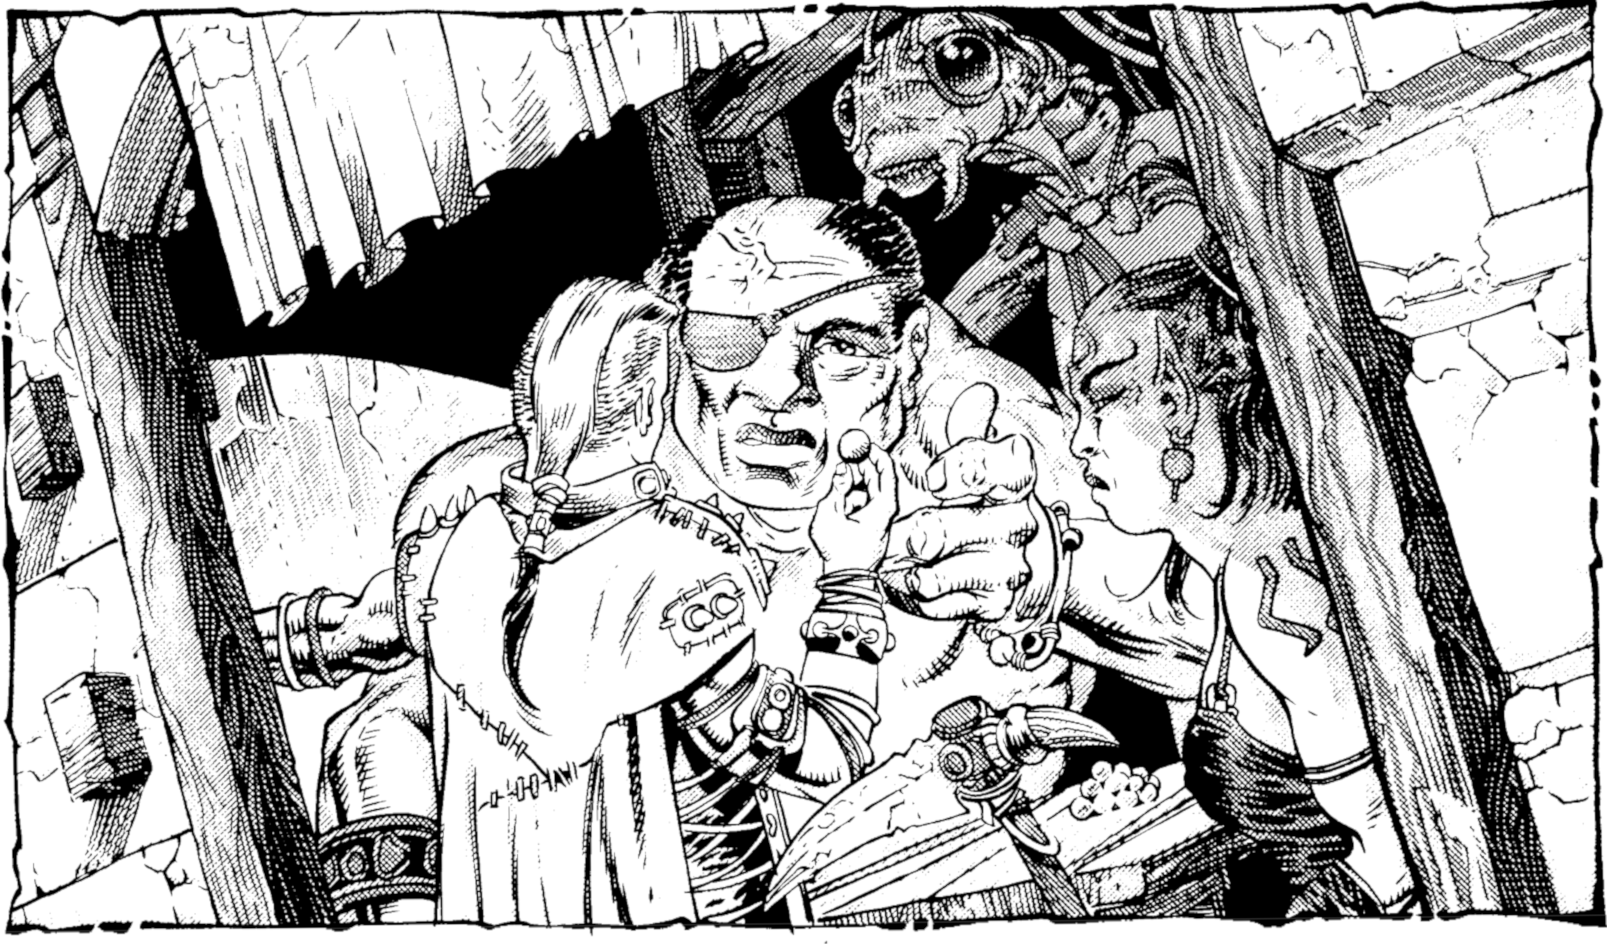
\includegraphics[width=\textwidth]{images/bribe-2.png}
\par\textit{\small\textcopyright Wizards of the Coast, 2020.}
\end{figure*}

\section{Wealth and Money}
\subsection{Coins}
All prices in {\tableheader Dark Sun} are given in terms of ceramic pieces, the most common coin. Ceramics are made from glazed clay and baked in batches once a year in a secure process supervised by the high templar that supervises the city's treasury. Bits are literally one-tenth parts of a ceramic piece---the ceramic pieces break easily into ten bits. Some cities' ceramic pieces have small holes that can be threaded onto a bracelet or necklace. The lowest unit of Athasian trade is the lead bead (bd).

Each of the city-states of the Tablelands produces its own currency. All cities use ceramic pieces as the most common coin, but also mint silver coins and, in some cases, rare and highly prized gold coins.

\Table{Currency Conversions}{l *4C}{
& \multicolumn{4}{c}{\tableheader Exchange Value}\\
\cmidrule[0.5pt]{2-5}
& \tableheader bd
& \tableheader bit
& \tableheader cp
& \tableheader sp\\
\textit{Lead bead (bd)}     & 1 & 1/10 & 1/100 & 1/1,000\\
\textit{Ceramic bit (bit)}  & 10 & 1 & 1/10 & 1/100\\
\textit{Ceramic piece (cp)} & 100 & 10 & 1 & 1/10\\
\textit{Silver piece (sp)}  & 1,000 & 100 & 10 & 1\\
\textit{Gold piece (gp)}    & 10,000 & 1000 & 100 & 10\\
}

\subsubsection{Moneychangers}
Adventurers that travel between cities will need to change their currency for local currency at each city they visit. With a couple of exceptions, the city-states have moneychangers available for incoming visitors. Located near the city gates and in large market places, moneychangers denote their business by hanging a large purple banner from their shop. The banners are always purple, but the moneychangers in each city-state display a different emblem on the banner, based on their city's standard.

Moneychangers charge each customer a fee to change coins. The fees differ by city and are summarized on \tabref{Moneychangers}.

\Table{Moneychangers}{C C}{
\tableheader City & \tableheader Exchange Rate\\
Balic   & 6\%\\
Draj    & 8\%\\
Gulg    & 10\%\\
Kurn    & 16\%\\
Nibenay & 14\%\\
Raam    & 12\%\\
Tyr     & 12\%\\
Urik    & 9\%\\
}

These fees are averages and may vary slightly. There are of course many unscrupulous money merchants who will charge as much as they can get away with. Moneychangers in Kurn are rare but a couple do exist. Since metal coins from any city-state are readily accepted by local merchants and no corresponding Kurnish coins exist there is little need to exchange such coins. There are, however, a few moneychangers willing to exchange ceramic pieces.

There are two cities that do not have moneychangers. Visitors to Celik have no need of a moneychangers, as merchants in that city take coins of all types. Nor are there any moneychangers in Eldaarich. Since Eldaarich has been shut off from the rest of the land for so long, visitors needing to exchange money have been nonexistent, so no moneychangers have set up business.

\subsection{Trade}
In general, the Athasian economy in the cities is relatively stable thanks to the Merchant Houses. Under normal conditions, supply is ample thanks to the caravans traveling back and forth between the cities. However, for smaller communities and trade outposts the price situation on certain goods can sway drastically. A raider attack or sandstorm can result in lack of necessities such as food and water, for which people will pay almost any amount of coin. Coins are not the only means of exchange. Barter and trade in commodities is widespread.

Dune traders commonly exchange trade goods without using currency, instead relying on a basic bartering system.


\Table{Trade Goods}{X r{1.3cm}}{
\tableheader Item & \tableheader Cost \\
One kilogram of salt & 4 bits \\
One kilogram of grain or faro & 6 bits \\
One kilogram of lead & 1 cp \\
One kilogram of nuts, or one kilogram of kank nectar & 2 cp \\
One square meter of cotton (cloth) & 4 cp \\
One kilogram of obsidian, or one square meter of silk, or one metric ton of water, or one erdlu & 10 cp \\
One herding kank, or one aprig & 50 cp \\
One kilogram of copper, or one male carru, or one inix & 100 cp \\
 One kilogram of iron, or one mekillot & 200 cp \\
One female carru & 300 cp \\
One kilogram of silver & 1,000 cp \\
One kilogram of gold & 10,000 cp \\
}

\subsection{Selling Loot}
In general, a character can sell something for half its listed price.

Trade goods are the exception to the half-price rule. A trade good, in this sense, is a valuable good that can be easily exchanged almost as if it were cash itself.

\section{Weapons}
Characters in a {\tableheader Dark Sun} game use a variety of weapons: some with direct counterparts in the real world, some without.

\subsection{Weapon Categories}
Weapons are grouped into several interlocking sets of categories.

These categories pertain to what training is needed to become proficient in a weapon's use (simple, martial, or exotic), the weapon's usefulness either in close combat (melee) or at a distance (ranged, which includes both thrown and projectile weapons), its relative encumbrance (light, one-handed, or two-handed), and its size (Small, Medium, or Large).

\textbf{Simple, Martial, and Exotic Weapons:} Anybody but a druid or wizard is proficient with all simple weapons. Barbarians, fighters, gladiators, and rangers are proficient with all simple and all martial weapons. Characters of other classes are proficient with an assortment of mainly simple weapons and possibly also some martial or even exotic weapons. A character who uses a weapon with which he or she is not proficient takes disadvantage on attack rolls.

\textbf{Melee and Ranged Weapons:} Melee weapons are used for making melee attacks, though some of them can be thrown as well. Ranged weapons are thrown weapons or projectile weapons that are not effective in melee.

\textit{Reach Weapons:} Glaives, guisarmes, lances, longspears, ranseurs, spiked chains, and whips are reach weapons. A reach weapon is a melee weapon that allows its wielder to strike at targets that aren't adjacent to him or her. Most reach weapons double the wielder's natural reach, meaning that a typical Small or Medium wielder of such a weapon can attack a creature 3 meters away, but not a creature in an adjacent square. A typical Large character wielding a reach weapon of the appropriate size can attack a creature 4.5 or 6 meters away, but not adjacent creatures or creatures up to 3 meters away.

Note: Small and Medium creatures wielding reach weapons threaten all squares 3 meters (2 squares) away, even diagonally. (This is an exception to the rule that 2 squares of diagonal distance is measured as 4.5 meters.)

\textit{Double Weapons:} Dire flails, dwarven urgroshes, gnome hooked hammers, orc double axes, quarterstaffs, and two-bladed swords are double weapons. A character can fight with both ends of a double weapon as if fighting with two weapons, but he or she incurs all the normal attack penalties associated with two-weapon combat, just as though the character were wielding a one-handed weapon and a light weapon.

The character can also choose to use a double weapon two handed, attacking with only one end of it. A creature wielding a double weapon in one hand can't use it as a double weapon---only one end of the weapon can be used in any given round.

\textit{Thrown Weapons:} Daggers, clubs, shortspears, spears, darts, javelins, throwing axes, light hammers, tridents, shuriken, and nets are thrown weapons. The wielder applies his or her Strength modifier to damage dealt by thrown weapons (except for splash weapons). It is possible to throw a weapon that isn't designed to be thrown (that is, a melee weapon that doesn't have a numeric entry in the Range Increment column on Table: Weapons), but a character who does so takes disadvantage on the attack roll. Throwing a light or one-handed weapon is a standard action, while throwing a two-handed weapon is a full-round action. Regardless of the type of weapon, such an attack scores a threat only on a natural roll of 20 and deals double damage on a critical hit. Such a weapon has a range increment of 3 meters.

\textit{Projectile Weapons:} Light crossbows, slings, heavy crossbows, shortbows, composite shortbows, longbows, composite longbows, hand crossbows, and repeating crossbows are projectile weapons. Most projectile weapons require two hands to use (see specific weapon descriptions). A character gets no Strength bonus on damage rolls with a projectile weapon unless it's a specially built composite shortbow, specially built composite longbow, or sling. If the character has a penalty for low Strength, apply it to damage rolls when he or she uses a bow or a sling.

\textit{Ammunition:} Projectile weapons use ammunition: arrows (for bows), bolts (for crossbows), or sling bullets (for slings). When using a bow, a character can draw ammunition as a free action; crossbows and slings require an action for reloading. Generally speaking, ammunition that hits its target is destroyed or rendered useless, while normal ammunition that misses has a 50\% chance of being destroyed or lost.

Although they are thrown weapons, shuriken are treated as ammunition for the purposes of drawing them, crafting masterwork or otherwise special versions of them (see Masterwork Weapons), and what happens to them after they are thrown.

\textbf{Light, One-Handed, and Two-Handed Melee Weapons:} This designation is a measure of how much effort it takes to wield a weapon in combat. It indicates whether a melee weapon, when wielded by a character of the weapon's size category, is considered a light weapon, a one-handed weapon, or a two-handed weapon.

\textit{Light:} A light weapon is easier to use in one's off hand than a one-handed weapon is, and it can be used while grappling. A light weapon is used in one hand. Add the wielder's Strength bonus (if any) to damage rolls for melee attacks with a light weapon if it's used in the primary hand, or one-half the wielder's Strength bonus if it's used in the off hand. Using two hands to wield a light weapon gives no advantage on damage; the Strength bonus applies as though the weapon were held in the wielder's primary hand only.

An unarmed strike is always considered a light weapon.

\textit{One-Handed:} A one-handed weapon can be used in either the primary hand or the off hand. Add the wielder's Strength bonus to damage rolls for melee attacks with a one-handed weapon if it's used in the primary hand, or \onehalf his or her Strength bonus if it's used in the off hand. If a one-handed weapon is wielded with two hands during melee combat, add 1\onehalf times the character's Strength bonus to damage rolls.

\textit{Two-Handed:} Two hands are required to use a two-handed melee weapon effectively. Apply 1\onehalf times the character's Strength bonus to damage rolls for melee attacks with such a weapon.

\textbf{Weapon Size:} Every weapon has a size category. This designation indicates the size of the creature for which the weapon was designed.

\Table{Larger and Smaller Weapon Damage}{l C C C C C}{
\tableheader Example Weapon & \tableheader Tiny & \tableheader Small & \tableheader Medium & \tableheader Large & \tableheader Huge \\
Shuriken & -- & 1 & 1d2 & 1d3 & 1d4\\
Gauntlet & 1 & 1d2 & 1d3 & 1d4 & 1d6\\
Dagger & 1d2 & 1d3 & 1d4 & 1d6 & 1d8\\
Shortspear & 1d3 & 1d4 & 1d6 & 1d8 & 2d6\\
Falchion & 1d4 & 1d6 & 2d4 & 2d6 & 3d6\\
Longsword & 1d4 & 1d6 & 1d8 & 2d6 & 3d6\\
Bastard Sword & 1d6 & 1d8 & 1d10 & 2d8 & 3d8\\
Greataxe & 1d8 & 1d10 & 1d12 & 3d6 & 4d6\\
Greatsword & 1d8 & 1d10 & 2d6 & 3d6 & 4d6\\
}

A weapon's size category isn't the same as its size as an object. Instead, a weapon's size category is keyed to the size of the intended wielder. In general, a light weapon is an object two size categories smaller than the wielder, a one-handed weapon is an object one size category smaller than the wielder, and a two-handed weapon is an object of the same size category as the wielder.

\textit{Inappropriately Sized Weapons:} A creature can't make optimum use of a weapon that isn't properly sized for it. A cumulative $-2$ penalty applies on attack rolls for each size category of difference between the size of its intended wielder and the size of its actual wielder. If the creature isn't proficient with the weapon disadvantage also applies.

The measure of how much effort it takes to use a weapon (whether the weapon is designated as a light, one-handed, or two-handed weapon for a particular wielder) is altered by one step for each size category of difference between the wielder's size and the size of the creature for which the weapon was designed. If a weapon's designation would be changed to something other than light, one-handed, or two-handed by this alteration, the creature can't wield the weapon at all.

\textbf{Improvised Weapons:} Sometimes objects not crafted to be weapons nonetheless see use in combat. Because such objects are not designed for this use, any creature that uses one in combat is considered to be nonproficient with it and takes disadvantage on attack rolls made with that object. To determine the size category and appropriate damage for an improvised weapon, compare its relative size and damage potential to the weapon list to find a reasonable match. An improvised weapon scores a threat on a natural roll of 20 and deals double damage on a critical hit. An improvised thrown weapon has a range increment of 3 meters.

\subsubsection{Metal Weapons}
Metal is rare on Athas, and many weapons ordinarily crafted using metal components are extremely expensive. Unworked iron is worth 100 cp per pound on average, but can cost much, much more in some places. Worked metal is even more expensive, as craftsmen who actually know how to craft metal items are rare at best. Most metal weapons are items dating back to the Green Age, or have been crafted from the meager resources of Tyr's iron mines.

Due to the rarity of metal, weapons and other items constructed primarily from metal are priced at in gp, e.g., a metal longsword costs 15 gp (or 1,500 cp). These weapons provide +1 bonus on damage rolls.

Due to the extremely high cost of metal weaponry, most weapons are constructed from inferior, but functional, materials instead on Athas. Most common are bone and stone such as flint or obsidian, but treated wood is sometimes used as well. Metal weapons constructed from inferior materials, such as bone longsword or an axe with a head made from stone, suffer a $-1$ penalty to attack and damage rolls. This penalty cannot reduce damage dealt below 1.

Furthermore, due to the rarity of metal, Athas has its share of unique weapons designed to be constructed from non-metal materials; as such, they do not suffer from the inferior materials penalties described above.

\NamedWeaponTable{Simple Weapons}{
\WeaponType{Unarmed Attacks}\\
Gauntlet
	& 2 cp & 4 cp & 1d2 & 1d3 & 1d4 & $\times2$ & & 0.25 kg& 0.5 kg& 1 kg & Bludgeoning\\
Unarmed strike
	& & & 1d2 & 1d3 & 1d4 & $\times2$ & & & & & Blud. non-lethal\\

\WeaponType{Light Melee Weapons}\\
Dagger
	& 2 cp & 4 cp & 1d3 & 1d4 & 1d6 & 19--20/$\times2$ & 3 m & 0.25 kg & 0.5 kg & 1 kg & Pierc. or slash.\\
Pushik
	& 4 cp & 8 cp & 1d3 & 1d4 & 1d6 & $\times3$ & & 0.25 kg & 0.5 kg & 1 kg & Piercing\\

\WeaponType{One-Handed Melee Weapons}\\
Club
	& & & 1d4 & 1d6 & 1d8 & $\times2$ & 3 m & 0.75 kg & 1.5 kg & 3 kg & Bludgeoning\\
Quabone
	& 3 cp & 6 cp & 1d4 & 1d6 & 1d8 & $\times2$ & & 1 kg & 2 kg & 4 kg & Bludgeoning\\
Shortspear
	& 1 cp & 2 cp & 1d4 & 1d6 & 1d8 & $\times2$ & 6 m & 0.75 kg & 1.5 kg & 3 kg & Piercing\\
Tonfa
	& 5 cp & 10 cp & 1d3 & 1d4 & 1d6 & $\times2$ & & 0.5 kg & 1 kg & 2 kg & Bludgeoning\\

\WeaponType{Two-Handed Melee Weapons}\\
Great tonfa
	& 10 cp & 20 cp & 1d4 & 1d6 & 1d8 & $\times2$ & & 1.25 kg & 2.5 kg & 5 kg & Bludgeoning\\
Longspear\footnotemark[1]
	& 5 cp & 10 cp & 1d6 & 1d8 & 2d6 & $\times3$ &  & 2.25 kg & 4.5 kg & 9 kg & Piercing\\
Quarterstaff\footnotemark[2]
	& & & 1d4 1d4 & 1d6 1d6 & 1d8 1d8 & $\times2$ & & 1 kg & 2 kg & 4 kg & Bludgeoning\\
Spear
	& 2 cp & 4 cp & 1d6 & 1d8 & 2d6 & $\times3$ & 6 m & 1.5 kg & 3 kg & 6 kg & Piercing\\

\WeaponType{Ranged Weapons}\\
Blowgun
	& 5 cp & 10 cp & 1 & 1d2 & 1d3 & $\times2$ & 3 m & 1 kg & 2 kg & 4 kg & Piercing\\
\Projectile{Needles, blowgun (20)}{1 cp}{2 cp}{}{}{}\\
Crossbow, heavy
	& 50 cp & 100 cp & 1d8 & 1d10 & 2d8 & 19--20/$\times2$ & 36 m & 2 kg & 4 kg & 8 kg & Piercing\\
\Projectile{Bolts, crossbow (10)}{1 cp}{2 cp}{0.25 kg}{0.5 kg}{1 kg}\\
Crossbow, light
	& 35 cp & 70 cp & 1d6 & 1d8 & 2d6 & 19--20/$\times2$ & 24 m & 1 kg & 2 kg & 4 kg & Piercing\\
\Projectile{Bolts, crossbow (10)}{1 cp}{2 cp}{0.25 kg}{0.5 kg}{1 kg}\\
Dart
	& 5 bits & 1 cp & 1d3 & 1d4 & 1d6 & $\times2$ & 6 m & 0.12 kg & 0.25 kg & 0.5 kg & Piercing\\
Javelin
	& 1 cp & 2 cp & 1d4 & 1d6 & 1d8 & $\times2$ & 9 m & 0.5 kg & 1 kg & 2 kg & Piercing\\
Pelota
	& 2 cp & 4 cp & 1d3 & 1d4 & 1d6 & $\times2$ & 3 m & 0.25 kg & 0.5 kg & 1 kg & Blud. and pierc.\\
Sling
	& & & 1d3 & 1d4 & 1d6 & $\times2$ & 15 m & & & & Bludgeoning\\
\Projectile{Bullets, sling (10)}{1 bit}{2 bits}{0.25 kg}{0.5 kg}{1 kg}\\

\BigTableNote{12}{1 Reach weapon}\\
\BigTableNote{12}{2 Double weapon}\\
}

\NamedWeaponTable{Martial Weapons}{
\WeaponType{Light Melee Weapons}\\
Forearm Axe
	& 30 cp & 60 cp & 1d3 & 1d4 & 1d6 & $\times3$ & & 1.5 kg & 3 kg & 6 kg & Slashing\\
Macahuitl, small
	& 20 cp & 40 cp & 1d4 & 1d6 & 1d8 & $\times2$ & & 0.5 kg & 1 kg & 2 kg & Slashing\\
Sap
	& 1 cp & 2 cp & 1d4 & 1d6 & 1d8 & $\times2$ & & 0.5 kg & 1 kg & 2 kg & Blud. non-lethal\\
Shield, light
	& $\star$ & $\star$ & 1d2 & 1d3 & 1d4 & $\times2$ & & $\star$ & $\star$ & $\star$ & Bludgeoning\\
Slodak
	& 18 cp & 36 cp & 1d4 & 1d6 & 1d8 & $\times2$ & & 1 kg & 2 kg & 4 kg & Slashing\\
Spiked armor
	& $\star$ & $\star$ & 1d4 & 1d6 & 1d8 & $\times2$ & & $\star$ & $\star$ & $\star$ & Piercing\\
Spiked shield, light
	& $\star$ & $\star$ & 1d3 & 1d4 & 1d6 & $\times2$ & & $\star$ & $\star$ & $\star$ & Piercing\\
Tortoise blade
	& 20 cp & 40 cp & 1d3 & 1d4 & 1d6 & 20/$\times2$ & & 0.5 kg & 1 kg & 2 kg & Piercing\\

\WeaponType{One-Handed Melee Weapons}\\
Alak
	& 7 cp & 14 cp & 1d4 & 1d6 & 1d8 & $\times3$ & & 1.5 kg & 3 kg & 6 kg & Piercing\\
Alhulak\footnotemark[1]
	& 40 cp & 80 cp & 1d4 & 1d6 & 1d8 & $\times3$ & & 2.25 kg & 4.5 kg & 9 kg & Piercing\\
Carrikal
	& 10 cp & 20 cp & 1d6 & 1d8 & 2d6 & $\times3$ & & 1.5 kg & 3 kg & 6 kg & Slashing\\
Impaler
	& 8 cp & 16 cp & 1d4 & 1d6 & 1d8 & $\times4$ & & 1.25 kg & 2.5 kg & 5 kg & Piercing\\
Macahuitl
	& 35 cp & 70 cp & 1d6 & 1d8 & 2d6 & $\times2$ & & 1.25 kg & 2.5 kg & 5 kg & Slashing\\
Shield, heavy
	& $\star$ & $\star$ & 1d3 & 1d4 & 1d6 & $\times2$ & & $\star$ & $\star$ & $\star$ & Bludgeoning\\
Spiked shield, heavy
	& $\star$ & $\star$ & 1d4 & 1d6 & 1d8 & $\times2$ & & $\star$ & $\star$ & $\star$ & Piercing\\

\WeaponType{Two-Handed Melee Weapons}\\
Club, datchi\footnotemark[1]
	& 5 cp & 10 cp & 1d6 & 1d8 & 2d6 & $\times3$ & & 2.5 kg & 5 kg & 10 kg & Bludgeoning\\
Crusher, Fixed\footnotemark[1]
	& 60 cp & 120 cp & 1d6 & 1d8 & 2d6 & $\times2$ & & 3 kg & 6 kg & 12 kg & Bludgeoning\\
Gouge
	& 20 cp & 40 cp & 1d8 & 1d10 & 2d8 & $\times3$ & & 3 kg & 6 kg & 12 kg & Piercing\\
Greatclub
	& 5 cp & 10 cp & 1d8 & 1d10 & 2d8 & $\times2$ & & 2 kg & 4 kg & 8 kg & Bludgeoning\\
Lance
	& 10 cp & 20 cp & 1d6 & 1d8 & 2d6 & $\times3$ & & 2.5 kg & 5 kg & 10 kg & Piercing\\
Macahuitl, Great
	& 50 cp & 100 cp & 1d10 & 2d6 & 3d6 & $\times2$ & & 3 kg & 6 kg & 12 kg & Slashing\\
Maul
	& 25 cp & 50 cp & 1d10 & 1d12 & 3d6 & $\times2$ & & 2.5 kg & 5 kg & 10 kg & Bludgeoning\\
Shield, long
	& $\star$ & $\star$ & 1d4 & 1d6 & 1d8 & $\times2$ & & $\star$ & $\star$ & $\star$ & Bludgeoning\\
Spiked shield, long
	& $\star$ & $\star$ & 1d6 & 1d8 & 2d6 & $\times2$ & & $\star$ & $\star$ & $\star$ & Piercing\\
Tkaesali\footnotemark[1]
	& 8 cp & 16 cp & 1d8 & 1d10 & 2d8 & $\times3$ & & 3.75 kg & 7.5 kg & 15 kg & Slashing\\
Trikal
	& 10 cp & 20 cp & 1d6 & 1d8 & 2d6 & $\times3$ & & 1.75 kg & 3.5 kg & 7 kg & Slashing\\

\WeaponType{Ranged Weapons}\\
Atlatl
	& 25 cp & 50 cp & 1d4 & 1d6 & 1d8 & $\times3$ & 12 m & 1.5 kg & 3 kg & 6 kg & Piercing\\
\Projectile{Javeli, atlatl}{2 cp}{4 cp}{0.5 kg}{1 kg}{2 kg}\\
Crossbow, fixed
	& 200 cp & 400 cp & 1d12 & 2d8 & 3d8 & 19--20/$\times2$ & 45 m & 25 kg & 50 kg & 100 kg & Piercing\\
\Projectile{Bolts (10)}{3 cp}{6 cp}{0.75 kg}{1.5 kg}{3 kg}\\
Longbow
	& 75 cp & 150 cp & 1d6 & 1d8 & 2d6 & $\times3$ & 30 m & 0.75 kg & 1.5 kg & 3 kg & Piercing\\
\Projectile{Arrows (10)}{1 cp}{2 cp}{0.75 kg}{1.5 kg}{3 kg}\\
Longbow, composite
	& 100 cp & 200 cp & 1d6 & 1d8 & 2d6 & $\times3$ & 33 m & 0.75 kg & 1.5 kg & 3 kg & Piercing\\
\Projectile{Arrows (10)}{1 cp}{2 cp}{0.75 kg}{1.5 kg}{3 kg}\\
Shortbow
	& 30 cp & 60 cp & 1d4 & 1d6 & 1d8 & $\times3$ & 18 m & 0.5 kg & 1 kg & 2 kg & Piercing\\
\Projectile{Arrows (10)}{1 cp}{2 cp}{0.75 kg}{1.5 kg}{3 kg}\\
Shortbow, composite
	& 75 cp & 150 cp & 1d4 & 1d6 & 1d8 & $\times3$ & 21 m & 0.5 kg & 1 kg & 2 kg & Piercing\\
\Projectile{Arrows (10)}{1 cp}{2 cp}{0.75 kg}{1.5 kg}{3 kg}\\

\BigTableNote{12}{1 Reach weapon}\\
\BigTableNote{12}{$\star$ Inherent properties of the armor or shield. See Armor for details.}\\
}

\NamedWeaponTable{Exotic Weapons}{
\WeaponType{Light Melee Weapons}\\
Bard's Friend
	& 20 cp & 40 cp & 1d3 & 1d4 & 1d6 & 18--20/$\times2$ & & 0.25 kg & 0.5 kg & 1 kg & Piercing\\
Bard's Garrote
	& 200 cp & 400 cp & 1d6 & 2d4 & 2d6 & $\times2$ & & 0.25 kg & 0.5 kg & 1 kg & Blud. non-lethal\\
Ko
	& 1 cp & 2 cp & 1d3 & 1d4 & 1d6 & $\times4$ & & 0.75 kg & 1.5 kg & 3 kg & Piercing\\
Handfork
	& 20 cp & 40 cp & 1d3 & 1d4 & 1d6 & $\times2$ & & 0.5 kg & 1 kg & 2 kg & Slashing\\
Lajav
	& 8 cp & 16 cp & 1d3 & 1d4 & 1d6 & $\times4$ & & 2 kg & 4 kg & 8 kg & Bludgeoning\\
Nunchaku
	& 2 cp & 4 cp & 1d4 & 1d6 & 1d8 & $\times2$ & & 0.5 kg & 1 kg & 2 kg & Bludgeoning\\
Sai
	& 1 cp & 2 cp & 1d3 & 1d4 & 1d6 & $\times2$ & 3 m & 0.25 kg & 0.5 kg & 1 kg & Bludgeoning\\
Singing Sticks
	& 10 cp & 20 cp & 1d4 & 1d6 & 1d8 & $\times2$ & & 0.25 kg & 0.5 kg & 1 kg & Bludgeoning\\
Talid
	& 40 cp & 80 cp & 1d4 & 1d6 & 1d8 & 19--20/$\times2$ & & 1 kg & 2 kg & 4 kg & Piercing\\
Widow's Knife
	& 50 cp & 100 cp & 1d3 & 1d4 & 1d6 & $\times3$ & & 0.5 kg & 1 kg & 2 kg & Piercing\\
Wrist Razor
	& 15 cp & 30 cp & 1d4 & 1d6 & 1d8 & 18--20/$\times2$ & & 0.5 kg & 1 kg & 2 kg & Slashing\\

\WeaponType{One-Handed Melee Weapons}\\
Heartpick
	& 9 cp & 18 cp & 1d6 & 1d8 & 2d6 & $\times4$ & & 0.5 kg & 1 kg & 2 kg & Piercing\\
Master's Whip\footnotemark[1]
	& 25 cp & 50 cp & 1d2 & 1d3 & 1d4 & $\times2$ & & 1.25 kg & 2.5 kg & 5 kg & Slashing\\
Whip\footnotemark[1]
	& 1 cp & 2 cp & 1d2 & 1d3 & 1d4 & $\times2$ & & 0.5 kg & 1 kg & 2 kg & Slash. non-lethal\\

\WeaponType{Two-Handed Melee Weapons}\\
Cahulak\footnotemark[2]
	& 120 cp & 240 cp & 1d4 1d4 & 1d6 1d6 & 1d8 1d8 & $\times3$ & & 3 kg & 6 kg & 12 kg & Piercing\\
Crusher, free\footnotemark[1]
	& 18 cp & 36 cp & 1d8 & 1d10 & 2d8 & $\times2$ & & 3 kg & 6 kg & 12 kg & Bludgeoning\\
Dragon's paw\footnotemark[2]
	& 80 cp & 160 cp & 1d4 1d4 & 1d6 1d6 & 1d8 1d8 & 19--20/$\times2$ & & 2.25 kg & 4.5 kg & 9 kg & Piercing\\
Gythka\footnotemark[2]
	& 60 cp & 120 cp & 1d6 1d6 & 1d8 1d8 & 2d6 2d6 & $\times2$ & & 6.25 kg & 12.5 kg & 25 kg & Slashing\\
Lotulis\footnotemark[2]
	& 115 cp & 230 cp & 1d6 1d6 & 1d8 1d8 & 2d6 2d6 & 19--20/$\times2$ & & 2.25 kg & 4.5 kg & 9 kg & Slashing\\
Pike, weighted\footnotemark[2]
	& 75 cp & 150 cp & 1d6 1d4 & 1d8 1d6 & 2d6 1d8 & 19--20/$\times2$ & & 3.75 kg & 7.5 kg & 15 kg & Bludgeoning Piercing\\
Spear, double-tipped\footnotemark[2]
	& 20 cp & 40 cp & 1d6 1d6 & 1d8 1d8 & 2d6 2d6 & $\times3$ & 6 m & 1.5 kg & 3 kg & 6 kg & Piercing\\
Thanak
	& 20 cp & 40 cp & 1d10 & 2d6 & 3d6 & $\times3$ & & 2.5 kg & 5 kg & 10 kg & Slashing\\
Swatter
	& 100 cp & 200 cp & 1d12 & 2d8 & 3d8 & $\times4$ & & 8.75 kg & 17.5 kg & 35 kg & Bludgeoning\\
Mekillot sap\footnotemark[1]
	& 25 cp & 50 cp & 1d12 & 2d8 & 3d8 & $\times2$ & 3 m & 7.5 kg & 15 kg & 30 kg & Blud. non-lethal\\

\WeaponType{Ranged Weapons}\\
Blowgun, greater
	& 10 cp & 20 cp & 1d3 & 1d4 & 1d6 & $\times2$ & 3 m & 1 kg & 2 kg & 4 kg & Piercing\\
\Projectile{Darts, blowgun (10)}{1 cp}{2 cp}{0.25 kg}{0.5 kg}{1 kg}\\
Bolas
	& 5 cp & 10 cp & 1d3 & 1d4 & 1d6 & $\times2$ & 3 m & 0.5 kg & 1 kg & 2 kg & Blud. non-lethal\\
Chatkcha
	& 20 cp & 40 cp & 1d4 & 1d6 & 1d8 & $\times2$ & 6 m & 0.75 kg & 1.5 kg & 3 kg & Piercing\\
Crossbow, hand
	& 100 cp & 200 cp & 1d3 & 1d4 & 1d6 & 19--20/$\times2$ & 9 m & 0.5 kg & 1 kg & 2 kg & Piercing\\
\Projectile{Bolts (10)}{1 cp}{2 cp}{0.25 kg}{0.5 kg}{1 kg}\\
Crossbow, repeat. heavy
	& 400 cp & 800 cp & 1d8 & 1d10 & 2d8 & 19--20/$\times2$ & 36 m & 3 kg & 6 kg & 12 kg & Piercing\\
\Projectile{Bolts (5)}{1 cp}{2 cp}{0.25 kg}{0.5 kg}{1 kg}\\
Crossbow, repeating light
	& 250 cp & 500 cp & 1d6 & 1d8 & 2d6 & 19--20/$\times2$ & 24 m & 1.5 kg & 3 kg & 6 kg & Piercing\\
\Projectile{Bolts (5)}{1 cp}{2 cp}{0.25 kg}{0.5 kg}{1 kg}\\
Dejada
	& 20 cp & 40 cp & 1d4 & 1d6 & 1d8 & $\times2$ & 9 m & 0.5 kg & 1 kg & 2 kg & Piercing\\
\Projectile{Pelota, dejada}{2 cp}{4 cp}{0.25 kg}{0.5 kg}{1 kg}\\
Lasso
	& 2 cp & 4 cp & & & & $\times2$ & 3 m & 0.5 kg & 1 kg & 2 kg & Bludgeoning\\
Net
	& 20 cp & 40 cp & & & & & 3 m & 1.5 kg & 3 kg & 6 kg & \\
Skyhammer
	& 50 cp & 100 cp & 1d8 & 1d10 & 2d8 & $\times2$ & 4.5 m & 1.5 kg & 3 kg & 6 kg & Bludgeoning\\
Splashbow
	& 300 cp & 600 cp & 1d3 & 1d4 & 1d6 & $\times2$ & 18 m & 15 kg & 30 kg & 60 kg & Bludgeoning\\
~ Pelota, hinged
	& 5 cp & 10 cp & & & & $\times2$ & 4.5 m & 0.5 kg & 1 kg & 2 kg & Bludgeoning\\
Zerka
	& 30 cp & 60 cp & 1d6 & 1d8 & 2d6 & 18--20/$\times2$ & 9 m & 2.25 kg & 4.5 kg & 9 kg & Piercing\\

\BigTableNote{12}{1 Reach weapon}\\
\BigTableNote{12}{2 Double weapon}\\
}

\NamedWeaponTable{Metal Simple Weapons}{
\WeaponType{Light Melee Weapons}\\
Dagger, punching
	& 2 gp & 4 gp & 1d3 & 1d4 & 1d6 & $\times3$ & & 0.25 kg & 0.5 kg & 1 kg & Piercing\\
\InferiorWeapon{(bone or wood)}{1 cp}{2 cp}{0.12 kg}{0.25 kg}{0.5 kg}\\
\InferiorWeapon{(stone)}{1 cp}{2 cp}{0.5 kg}{1 kg}{2 kg}\\
Gauntlet, spiked
	& 25 sp & 5 gp & 1d3 & 1d4 & 1d6 & $\times2$ & & 0.25 kg & 0.5 kg & 1 kg & Piercing\\
\InferiorWeapon{(bone or wood)}{25 bits}{5 cp}{0.12 kg}{0.25 kg}{0.5 kg}\\
\InferiorWeapon{(stone)}{25 bits}{5 cp}{0.5 kg}{1 kg}{2 kg}\\
Mace, light
	& 5 gp & 10 gp & 1d4 & 1d6 & 1d8 & $\times2$ & & 1 kg & 2 kg & 4 kg & Bludgeoning\\
\InferiorWeapon{(bone or wood)}{25 bits}{5 cp}{0.5 kg}{1 kg}{2 kg}\\
\InferiorWeapon{(stone)}{25 bits}{5 cp}{2 kg}{4 kg}{8 kg}\\
Sickle
	& 6 gp & 12 gp & 1d4 & 1d6 & 1d8 & $\times2$ & & 0.5 kg & 1 kg & 2 kg & Slashing\\
\InferiorWeapon{(bone or wood)}{1 cp}{2 cp}{0.25 kg}{0.5 kg}{1 kg}\\
\InferiorWeapon{(stone)}{1 cp}{2 cp}{1 kg}{2 kg}{4 kg}\\

\WeaponType{One-Handed Melee Weapons}\\
Mace, heavy
	& 12 gp & 24 cp & 1d6 & 1d8 & 2d6 & $\times2$ & & 2 kg & 4 kg & 8 kg & Bludgeoning\\
\InferiorWeapon{(bone or wood)}{6 cp}{12 cp}{1 kg}{2 kg}{4 kg}\\
\InferiorWeapon{(stone)}{6 cp}{12 cp}{4 kg}{8 kg}{16 kg}\\
Morningstar
	& 8 gp & 16 gp & 1d6 & 1d8 & 2d6 & $\times2$ & & 1.5 kg & 3 kg & 6 kg & Blud. and pierc.\\
\InferiorWeapon{(bone or wood)}{4 cp}{8 cp}{0.75 kg}{1.5 kg}{3 kg}\\
\InferiorWeapon{(stone)}{4 cp}{8 cp}{3 kg}{6 kg}{12 kg}\\

\BigTableNote{12}{$\diamond$ Inferior material weapons suffer $-1$ penalty to attack and damage rolls.}\\
% \rowcolor{white}\\
\rowcolor{white}\\
}

\NamedWeaponTable{Metal Martial Weapons 1}{
\WeaponType{Light Melee Weapons}\\
Axe, throwing
	& 8 gp & 16 gp & 1d4 & 1d6 & 1d6 & $\times2$ & 3 m & 0.5 kg & 1 kg & 2 kg & Slashing\\
\InferiorWeapon{(bone or wood)}{4 cp}{8 cp}{0.25 kg}{0.5 kg}{1 kg}\\
\InferiorWeapon{(stone)}{4 cp}{8 cp}{1 kg}{2 kg}{4 kg}\\
Hammer, light
	& 1 gp & 2 gp & 1d3 & 1d4 & 1d4 & $\times2$ & 6 m & 0.5 kg & 1 kg & 2 kg & Bludgeoning\\
\InferiorWeapon{(bone or wood)}{5 bits}{1 cp}{0.25 kg}{0.5 kg}{1 kg}\\
\InferiorWeapon{(stone)}{5 bits}{1 cp}{1 kg}{2 kg}{4 kg}\\
Handaxe
	& 6 gp & 12 gp & 1d4 & 1d6 & 1d6 & $\times3$ & & 0.75 kg & 1.5 kg & 3 kg & Slashing\\
\InferiorWeapon{(bone or wood)}{3 cp}{6 cp}{0.37 kg}{0.75 kg}{1.5 kg}\\
\InferiorWeapon{(stone)}{3 cp}{6 cp}{1.5 kg}{3 kg}{6 kg}\\
Kukri
	& 8 gp & 16 gp & 1d3 & 1d4 & 1d6 & 18--20/$\times2$ & & 0.5 kg & 1 kg & 2 kg & Slashing\\
\InferiorWeapon{(bone or wood)}{4 cp}{8 cp}{0.25 kg}{0.5 kg}{1 kg}\\
\InferiorWeapon{(stone)}{4 cp}{8 cp}{1 kg}{2 kg}{4 kg}\\
Pick, light
	& 4 gp & 8 gp & 1d3 & 1d4 & 1d6 & $\times4$ & & 0.75 kg & 1.5 kg & 3 kg & Piercing\\
\InferiorWeapon{(bone or wood)}{2 cp}{4 cp}{0.37 kg}{0.75 kg}{1.5 kg}\\
\InferiorWeapon{(stone)}{2 cp}{4 cp}{1.5 kg}{3 kg}{6 kg}\\
Sword, short
	& 10 gp & 20 gp & 1d4 & 1d6 & 1d8 & 19--20/$\times2$ & & 0.5 kg & 1 kg & 2 kg & Piercing\\
\InferiorWeapon{(bone or wood)}{5 cp}{10 cp}{0.25 kg}{0.5 kg}{1 kg}\\
\InferiorWeapon{(stone)}{5 cp}{10 cp}{1 kg}{2 kg}{4 kg}\\

\WeaponType{One-Handed Melee Weapons}\\
Battleaxe
	& 10 gp & 20 gp & 1d6 & 1d8 & 2d6 & $\times3$ & & 1.5 kg & 3 kg & 6 kg & Slashing\\
\InferiorWeapon{(bone or wood)}{5 cp}{10 cp}{0.75 kg}{1.5 kg}{3 kg}\\
\InferiorWeapon{(stone)}{5 cp}{10 cp}{3 kg}{6 kg}{12 kg}\\
Flail
	& 8 gp & 16 gp & 1d6 & 1d8 & 2d6 & $\times2$ & & 1.25 kg & 2.5 kg & 5 kg & Bludgeoning\\
\InferiorWeapon{(bone or wood)}{4 cp}{8 cp}{0.62 kg}{1.25 kg}{2.5 kg}\\
\InferiorWeapon{(stone)}{4 cp}{8 cp}{2.5 kg}{5 kg}{10 kg}\\
Longsword
	& 15 gp & 30 gp & 1d6 & 1d8 & 2d6 & 19--20/$\times2$ & & 1 kg & 2 kg & 4 kg & Slashing\\
\InferiorWeapon{(bone or wood)}{75 bits}{15 cp}{0.5 kg}{1 kg}{2 kg}\\
\InferiorWeapon{(stone)}{75 bits}{15 cp}{2 kg}{4 kg}{8 kg}\\
Pick, heavy
	& 8 gp & 16 gp & 1d4 & 1d6 & 1d8 & $\times4$ & & 1.5 kg & 3 kg & 6 kg & Piercing\\
\InferiorWeapon{(bone or wood)}{4 cp}{8 cp}{0.75 kg}{1.5 kg}{3 kg}\\
\InferiorWeapon{(stone)}{4 cp}{8 cp}{3 kg}{6 kg}{12 kg}\\
Rapier
	& 20 gp & 40 gp & 1d4 & 1d6 & 1d8 & 18--20/$\times2$ & & 0.5 kg & 1 kg & 2 kg & Piercing\\
\InferiorWeapon{(bone or wood)}{10 cp}{20 cp}{0.25 kg}{0.5 kg}{1 kg}\\
\InferiorWeapon{(stone)}{10 cp}{20 cp}{1 kg}{2 kg}{4 kg}\\
Scimitar
	& 15 gp & 30 gp & 1d4 & 1d6 & 1d8 & 18--20/$\times2$ & & 1 kg & 2 kg & 4 kg & Slashing\\
\InferiorWeapon{(bone or wood)}{75 bits}{15 cp}{0.5 kg}{1 kg}{2 kg}\\
\InferiorWeapon{(stone)}{75 bits}{15 cp}{2 kg}{4 kg}{8 kg}\\
Trident
	& 15 gp & 30 gp & 1d6 & 1d8 & 2d6 & $\times2$ & 3 m & 1 kg & 2 kg & 4 kg & Piercing\\
\InferiorWeapon{(bone or wood)}{75 bits}{15 cp}{0.5 kg}{1 kg}{2 kg}\\
\InferiorWeapon{(stone)}{75 bits}{15 cp}{2 kg}{4 kg}{8 kg}\\
Warhammer
	& 12 gp & 24 gp & 1d6 & 1d8 & 2d6 & $\times3$ & & 1.25 kg & 2.5 kg & 5 kg & Bludgeoning\\
\InferiorWeapon{(bone or wood)}{6 cp}{12 cp}{0.62 kg}{1.25 kg}{2.5 kg}\\
\InferiorWeapon{(stone)}{6 cp}{12 cp}{2.5 kg}{5 kg}{10 kg}\\

\BigTableNote{12}{$\diamond$ Inferior material weapons suffer $-1$ penalty to attack and damage rolls.}\\
\rowcolor{white}\\
\rowcolor{white}\\
}

\NamedWeaponTable{Metal Martial Weapons 2}{
\WeaponType{Two-Handed Melee Weapons}\\
Falchion
	& 75 gp & 150 gp & 1d6 & 2d4 & 2d6 & 18--20/$\times2$ & & 2 kg & 4 kg & 8 kg & Slashing\\
\InferiorWeapon{(bone or wood)}{32.5 cp}{75 cp}{1 kg}{2 kg}{4 kg}\\
\InferiorWeapon{(stone)}{32.5 cp}{75 cp}{4 kg}{8 kg}{16 kg}\\
Glaive\footnotemark[1]
	& 8 gp & 16 gp & 1d8 & 1d10 & 2d8 & $\times3$ & & 2.5 kg & 5 kg & 10 kg & Slashing\\
\InferiorWeapon{(bone or wood)}{4 cp}{8 cp}{1.25 kg}{2.5 kg}{5 kg}\\
\InferiorWeapon{(stone)}{4 cp}{8 cp}{5 kg}{10 kg}{20 kg}\\
Greataxe
	& 20 gp & 40 gp & 1d10 & 1d12 & 3d6 & $\times3$ & & 3 kg & 6 kg & 12 kg & Slashing\\
\InferiorWeapon{(bone or wood)}{10 cp}{20 cp}{1.5 kg}{3 kg}{6 kg}\\
\InferiorWeapon{(stone)}{10 cp}{20 cp}{6 kg}{12 kg}{24 kg}\\
Flail, heavy
	& 15 gp & 30 gp & 1d8 & 1d10 & 2d8 & 19--20/$\times2$ & & 2.5 kg & 5 kg & 10 kg & Bludgeoning\\
\InferiorWeapon{(bone or wood)}{75 bits}{15 cp}{1.25 kg}{2.5 kg}{5 kg}\\
\InferiorWeapon{(stone)}{75 bits}{15 cp}{5 kg}{10 kg}{20 kg}\\
Greatsword
	& 50 gp & 100 gp & 1d10 & 2d6 & 3d6 & 19--20/$\times2$ & & 2 kg & 4 kg & 8 kg & Slashing\\
\InferiorWeapon{(bone or wood)}{25 cp}{50 cp}{1 kg}{2 kg}{4 kg}\\
\InferiorWeapon{(stone)}{25 cp}{50 cp}{4 kg}{8 kg}{16 kg}\\
Guisarme\footnotemark[1]
	& 45 sp & 9 gp & 1d6 & 2d4 & 2d6 & $\times3$ & & 3 kg & 6 kg & 12 kg & Slashing\\
\InferiorWeapon{(bone or wood)}{25 bits}{45 bits}{0.25 kg}{0.5 kg}{1 kg}\\
\InferiorWeapon{(stone)}{25 bits}{45 bits}{1 kg}{2 kg}{4 kg}\\
Halberd
	& 10 gp & 20 gp & 1d8 & 1d10 & 2d8 & $\times3$ & & 3 kg & 6 kg & 12 kg & Pierc. or slash.\\
\InferiorWeapon{(bone or wood)}{5 cp}{10 cp}{1.5 kg}{3 kg}{6 kg}\\
\InferiorWeapon{(stone)}{5 cp}{10 cp}{6 kg}{12 kg}{24 kg}\\
Ranseur\footnotemark[1]
	& 10 gp & 20 gp & 1d6 & 2d4 & 2d6 & $\times3$ & & 3 kg & 6 kg & 12 kg & Piercing\\
\InferiorWeapon{(bone or wood)}{5 cp}{10 cp}{1.5 kg}{3 kg}{6 kg}\\
\InferiorWeapon{(stone)}{5 cp}{10 cp}{6 kg}{12 kg}{24 kg}\\
Scythe
	& 18 gp & 36 gp & 1d6 & 2d4 & 2d6 & $\times4$ & & 2.5 kg & 5 kg & 10 kg & Pierc. or slash.\\
\InferiorWeapon{(bone or wood)}{9 cp}{18 cp}{1.25 kg}{2.5 kg}{5 kg}\\
\InferiorWeapon{(stone)}{9 cp}{18 cp}{5 kg}{10 kg}{20 kg}\\

\WeaponType{Ranged Weapons}\\
\Projectile{Arrows, metal (20)}{1 gp}{2 gp}{0.75 kg}{1.5 kg}{3 kg}\\


\BigTableNote{12}{1 Reach weapon}\\
\BigTableNote{12}{$\diamond$ Inferior material weapons suffer $-1$ penalty to attack and damage rolls.}\\
}

\NamedWeaponTable{Metal Exotic Weapons}{
\WeaponType{Light Melee Weapons}\\
Kama
	& 2 gp & 4 gp & 1d4 & 1d6 & 1d8 & $\times2$ & & 0.5 kg & 1 kg & 2 kg & Slashing\\
\InferiorWeapon{(bone or wood)}{1 cp}{2 cp}{0.25 kg}{0.5 kg}{1 kg}\\
\InferiorWeapon{(stone)}{1 cp}{2 cp}{1 kg}{2 kg}{4 kg}\\
\WeaponType{One-Handed Melee Weapons}\\
Longblade, elven
	& 15 gp & 30 gp & 1d6 & 1d8 & 2d6 & 18--20/$\times2$ & & 0.75 kg & 1.5 kg & 3 kg & Slashing\\
\InferiorWeapon{(bone or wood)}{8 cp}{15 cp}{0.37 kg}{0.75 kg}{1.5 kg}\\
\InferiorWeapon{(stone)}{8 cp}{15 cp}{1.5 kg}{3 kg}{6 kg}\\
Sword, bastard
	& 35 gp & 70 gp & 1d8 & 1d10 & 2d8 & 19--20/$\times2$ & & 1.5 kg & 3 kg & 6 kg & Slashing\\
\InferiorWeapon{(bone or wood)}{18 cp}{35 cp}{0.75 kg}{1.5 kg}{3 kg}\\
\InferiorWeapon{(stone)}{18 cp}{35 cp}{3 kg}{6 kg}{12 kg}\\
Waraxe, dwarven
	& 30 gp & 60 gp & 1d8 & 1d10 & 2d8 & $\times3$ & & 2 kg & 4 kg & 8 kg & Slashing\\
\InferiorWeapon{(bone or wood)}{15 cp}{30 cp}{1 kg}{2 kg}{4 kg}\\
\InferiorWeapon{(stone)}{15 cp}{30 cp}{4 kg}{8 kg}{16 kg}\\

\WeaponType{Two-Handed Melee Weapons}\\
Chain, spiked\footnotemark[1]
	& 25 gp & 50 gp & 1d6 & 2d4 & 2d6 & $\times2$ & & 2.5 kg & 5 kg & 10 kg & Piercing\\
\InferiorWeapon{(bone or wood)}{13 cp}{25 cp}{1.25 kg}{2.5 kg}{5 kg}\\
\InferiorWeapon{(stone)}{13 cp}{25 cp}{5 kg}{10 kg}{20 kg}\\
Flail, dire
	& 90 gp & 180 gp & 1d6 1d6 & 1d8 1d8 & 2d6 2d6 & $\times2$ & & 2.5 kg & 5 kg & 10 kg & Bludgeoning\\
\InferiorWeapon{(bone or wood)}{45 cp}{90 cp}{1.25 kg}{2.5 kg}{5 kg}\\
\InferiorWeapon{(stone)}{45 cp}{90 cp}{5 kg}{10 kg}{20 kg}\\
Sword, two-bladed\footnotemark[2]
	& 100 gp & 200 gp & 1d6 1d6 & 1d8 1d8 & 2d6 2d6 & 19--20/$\times2$ & & 2.5 kg & 5 kg & 10 kg & Slashing\\
\InferiorWeapon{(bone or wood)}{45 cp}{90 cp}{1.25 kg}{2.5 kg}{5 kg}\\
\InferiorWeapon{(stone)}{45 cp}{90 cp}{5 kg}{10 kg}{20 kg}\\
Urgrosh, dwarven\footnotemark[2]
	& 50 gp & 100 gp & 1d6 1d4 & 1d8 1d6 & 2d6 1d8 & $\times3$ & & 3 kg & 6 kg & 12 kg & Slashing Piercing\\
\InferiorWeapon{(bone or wood)}{25 cp}{50 cp}{1.5 kg}{3 kg}{6 kg}\\
\InferiorWeapon{(stone)}{25 cp}{50 cp}{6 kg}{12 kg}{24 kg}\\

\WeaponType{Ranged Weapons}\\
Shuriken (5)
	& 1 gp & 2 gp & 1 & 1d2 & 1d3 & $\times2$ & 3 m & 0.25 kg & 0.5 kg & 1 kg & Piercing\\
\InferiorWeapon{(bone or wood)}{5 bits}{1 cp}{0.12 kg}{0.25 kg}{0.5 kg}\\
\InferiorWeapon{(stone)}{5 bits}{1 cp}{0.5 kg}{1 kg}{2 kg}\\

\BigTableNote{12}{1 Reach weapon}\\
\BigTableNote{12}{2 Double weapon}\\
\BigTableNote{12}{$\diamond$ Inferior material weapons suffer $-1$ penalty to attack and damage rolls.}\\
}



\subsection{Weapon Qualities}
Here is the format for weapon entries (given as column headings on each weapon table).

\textbf{Cost:} This value is the weapon's cost in gold pieces (gp), silver pieces (sp), ceramic pieces (cp) or ceramic bits (bits). The cost includes miscellaneous gear that goes with the weapon.

This cost is the same for a Small or Medium version of the weapon. A Large version costs twice the listed price.

\textbf{Damage:} The Damage columns give the damage dealt by the weapon on a successful hit. There are three columns for different weapon sizes: ``S'' for Small weapons, ``M'' for Medium weapons, and ``L'' for Large weapons. If two damage ranges are given then the weapon is a double weapon. Use the second damage figure given for the double weapon's extra attack. \tabref{Larger and Smaller Weapon Damage} gives weapon damage values for weapons of various sizes.

\textbf{Critical:} The entry in this column notes how the weapon is used with the rules for critical hits. When your character scores a critical hit, roll the damage two, three, or four times, as indicated by its critical multiplier (using all applicable modifiers on each roll), and add all the results together.

\textit{Exception:} Extra damage over and above a weapon's normal damage is not multiplied when you score a critical hit.

\textit{\multiplied2:} The weapon deals double damage on a critical hit.

\textit{\multiplied3:} The weapon deals triple damage on a critical hit.

\textit{\multiplied4:} The weapon deals quadruple damage on a critical hit.

\textit{19--20/\multiplied2:} The weapon scores a threat on a natural roll of 19 or 20 (instead of just 20) and deals double damage on a critical hit. (The weapon has a threat range of 19--20.)

\textit{18--20/\multiplied2:} The weapon scores a threat on a natural roll of 18, 19, or 20 (instead of just 20) and deals double damage on a critical hit. (The weapon has a threat range of 18--20.)

\textbf{Range Increment:} Any attack at less than this distance is not penalized for range. However, each full range increment imposes a cumulative $-2$ penalty on the attack roll. A thrown weapon has a maximum range of five range increments. A projectile weapon can shoot out to ten range increments.

\textbf{Weight:} There are three columns for the weight of a weapon: ``S'' for Small weapons, ``M'' for Medium weapons, and ``L'' for Large weapons.

\textbf{Type:} Weapons are classified according to the type of damage they deal: bludgeoning, piercing, or slashing. Some monsters may be resistant or immune to attacks from certain types of weapons.

Some weapons deal damage of multiple types. If a weapon is of two types, the damage it deals is not half one type and half another; all of it is both types. Therefore, a creature would have to be immune to both types of damage to ignore any of the damage from such a weapon.

In other cases, a weapon can deal either of two types of damage. In a situation when the damage type is significant, the wielder can choose which type of damage to deal with such a weapon.

\textbf{Special:} Some weapons have special features. See the weapon descriptions for details.

\subsection{Weapon Descriptions}
Weapons found on \tabref{Weapons} that have special options for the wielder (``you'') are described below. Splash weapons are described under Special Substances and Items.

\textbf{Alak:} An alak consists of a 60 centemeters long shaft of bone or wood, with four serrated bones tied to the sharp end, like the four prongs of a grappling hook.

When using an alak, you get a +2 bonus on the opposed attack roll when attempting to disarm an opponent (including the roll to avoid being disarmed if you fail to disarm your opponent). 

\textbf{Alhulak:} The alhulak consists of an alak tied to a 1.5 meter long leather cord, which wraps around your wrist at the other end. An alhulak has reach. You can strike opponents 3 meters away with it. In you getition, you can use it against an adjacent foe.

When using an alhulak, you get a +2 bonus on the opposed attack roll when attempting to disarm an opponent (including the roll to avoid being disarmed if the character fails to disarm his or her opponent). 

\textbf{Arrows:} An arrow used as a melee weapon is treated as a light improvised weapon ($-4$ penalty on attack rolls) and deals damage as a dagger of its size (critical multiplier $\times$2). Arrows come in a leather quiver that holds 20 arrows. An arrow that hits its target is destroyed; one that misses has a 50\% chance of being destroyed or lost. 

\textbf{Atlatl:} The atlatl, sometimes called a ``staff-sling,'' is a javelin-throwing device that is swung over the shoulder, using both hands. Javelins flung with an atlatl gain greater range than those thrown by hand. 

\textbf{Bard's Friend:} This weapon is crafted with several obsidian blades and wooden prongs, which are fastened to a handle. Several small spikes jut out from where the knuckles hold the weapon. Bards are known for smearing these spikes with injury poison. The bard's friend can be coated with three charges of poison, but only one may be delivered per attack made with the weapon. 

\textbf{Blowgun, Greater:} The greater blowgun fires blowgun darts, which are slightly smaller than thrown darts, and are capable of delivering poison as well. 

\textbf{Blowgun:} The blowgun is a long tube through which you blow air to fire needles. The needles don't deal much damage, but are often coated in poison. 

\textbf{Bolas:} You can use this weapon to make a ranged trip attack against an opponent. You can't be tripped during your own trip attempt when using a set of bolas. 

\textbf{Bolts:} A crossbow bolt used as a melee weapon is treated as a light improvised weapon ($-4$ penalty on attack rolls) and deals damage as a dagger of its size (crit $\times$2). Bolts come in a wooden case that holds 10 bolts (or 5, for a repeating crossbow). A bolt that hits its target is destroyed; one that misses has a 50\% chance of being destroyed or lost. 

\textbf{Bullets, Sling:} Bullets come in a leather pouch that holds 10 bullets. A bullet that hits its target is destroyed; one that misses has a 50\% chance of being destroyed or lost. 

\textbf{Cahulak:} A cahulak consists of two alaks (see above) joined by a 1.5 meter rope. You may fight as if fighting with two weapons, but if you do, you incur all the normal attack penalties associated with fighting with a light offhand weapon. A creature using a double weapon in one hand, such as a half-giant using a set of cahulaks can't use it as a double weapon.

When using a cahulak, you get a +2 bonus on the opposed attack roll when attempting to disarm an opponent (including the roll to avoid being disarmed if the character fails to disarm his or her opponent).

Because the cahulak can wrap around an enemy's leg or other limb, you can make trip attacks with it. If you are tripped during your own trip attempt, you can drop the cahulak to avoid being tripped.

If you strike at an opponent 3 meters away, you cannot use the cahulak as a double weapon unless you possess natural reach. 

\textbf{Carrikal:} The sharpened jawbone of a large creature is lashed to a haft. The jagged edges are sharpened, forming a sort of battleaxe with two forward-facing heads.

\textbf{Chain, Spiked:} A spiked chain has reach, so you can strike opponents 3 meters away with it. In addition, unlike most other weapons with reach, it can be used against an adjacent foe.

You can make trip attacks with the chain. If you are tripped during your own trip attempt, you can drop the chain to avoid being tripped.

When using a spiked chain, you get a +2 bonus on opposed attack rolls made to disarm an opponent (including the roll to avoid being disarmed if such an attempt fails).

You can use the \feat{Weapon Finesse} feat to apply your Dexterity modifier instead of your Strength modifier to attack rolls with a spiked chain sized for you, even though it isn't a light weapon for you. 

\textbf{Chatkcha:} The chatkcha returns to a proficient thrower on a missed attack roll. To catch it, the character must make an attack roll against AC 10 using the same bonus they threw the chatkcha with. Failure indicates the weapon falls to the ground 3 meters in a random direction from the thrower. Catching the chatkcha is part of the attack and does not count as a separate attack.

\textbf{Crossbow, Fixed:} This version of the crossbow can be fired by any capable of using it, but cannot be carried like a conventional crossbow. It is fixed in place, i.e. mounted on top of a wall, pole, or vehicle, and swivels so that you can aim the shot. Crossbows at the edge of a caravan, cart, or wall tend to offer cover, but limit your range of firing to a cone shape directly in front of the weapon.

It is possible to mount a fixed crossbow on top of a pole but inside a shallow pit, giving you a 360-degree range of motion, while giving you cover. In any case, it is impossible to swivel a fixed crossbow in order to attack upwards (your upward angle is limited to 45 degrees). Reloading a fixed crossbow is a full-round action.

\textbf{Crossbow, Hand:} You can draw a hand crossbow back by hand. Loading a hand crossbow is a move action that provokes attacks of opportunity.

You can shoot, but not load, a hand crossbow with one hand at no penalty. You can shoot a hand crossbow with each hand, but you take a penalty on attack rolls as if attacking with two light weapons. 

\textbf{Crossbow, Heavy:} You draw a heavy crossbow back by turning a small winch. Loading a heavy crossbow is a full-round action that provokes attacks of opportunity.

Normally, operating a heavy crossbow requires two hands. However, you can shoot, but not load, a heavy crossbow with one hand at a $-4$ penalty on attack rolls. You can shoot a heavy crossbow with each hand, but you take a penalty on attack rolls as if attacking with two one-handed weapons. This penalty is cumulative with the penalty for one-handed firing. 

\textbf{Crossbow, Light:} You draw a light crossbow back by pulling a lever. Loading a light crossbow is a move action that provokes attacks of opportunity.

Normally, operating a light crossbow requires two hands. However, you can shoot, but not load, a light crossbow with one hand at a $-2$ penalty on attack rolls. You can shoot a light crossbow with each hand, but you take a penalty on attack rolls as if attacking with two light weapons. This penalty is cumulative with the penalty for one-handed firing. 

\textbf{Crossbow, Repeating:} The repeating crossbow (whether heavy or light) holds 5 crossbow bolts. As long as it holds bolts, you can reload it by pulling the reloading lever (a free action). Loading a new case of 5 bolts is a full-round action that provokes attacks of opportunity.

You can fire a repeating crossbow with one hand or fire a repeating crossbow in each hand in the same manner as you would a normal crossbow of the same size. However, you must fire the weapon with two hands in order to use the reloading lever, and you must use two hands to load a new case of bolts. 

\textbf{Crusher:} The crusher is made from a large stone or metal weight, mounted at the end of a 4.5 meters long shaft of springy wood. The weight is whipped back and forth. The crusher is a reach weapon. You can strike opponents 3 meters away with it, but you cannot use it against an adjacent foe. You need a 4.5 meters ceiling to use the weapon, but it can reach over cover.

Crushers come in two varieties, fixed and free. A fixed crusher requires a base to use. The fixed crusher's base is enormously heavy, usually consisting of a thick slab of stone with a hole drilled through it to support the crusher's pole. The base is transported separately from the pole, and it takes one full minute to set the fixed crusher up for battle. The fixed crusher is a martial weapon, finding most use in infantry units.

It is possible to use the crusher pole without the base as a free crusher, but this requires considerable expertise. You need an exotic weapon proficiency in the free crusher to accomplish this feat without the $-4$ proficiency penalty, even if you are proficient in the fixed crusher.

\textbf{Dagger:} You get a +2 bonus on Sleight of Hand checks made to conceal a dagger on your body (see the Sleight of Hand skill). 

\textbf{Datchi Club:} A datchi club has reach. You can strike opponents 3 meters away with it, but you cannot use it against an adjacent foe. This weapon, generally found in the arenas, is made by affixing a 1.2-$-1$.5 meter length of dried insect hive or roots to a 90 centimeters long shaft. Teeth, claws, or obsidian shards are embedded into the head of the weapon.

\textbf{Dejada:} The dejada allows the wielder to throw pelota (see the pelota description for details). These pelotas deal more damage than those thrown by hand, due to the great speed at which they are thrown from a dejada.

\textbf{Dragon's Paw:} Popular in the arenas, the dragon's paw consists of a 1.5-$-1$.8 meter long pole, with a blade on either end. A basket guards your hands from attack, granting a +2 bonus on all attempts to defend against being disarmed.

A dragon's paw is a double weapon. You may fight as if fighting with two weapons, but if you do, you incur all the normal attack penalties associated with fighting with a light off-hand weapon. A creature using a double weapon in one hand, such as a half-giant using a dragon's paw can't use it as a double weapon.

\textbf{Flail or Heavy Flail:} With a flail, you get a +2 bonus on opposed attack rolls made to disarm an enemy (including the roll to avoid being disarmed if such an attempt fails).

You can also use this weapon to make trip attacks. If you are tripped during your own trip attempt, you can drop the flail to avoid being tripped. 

\textbf{Flail, Dire:} A dire flail is a double weapon. You can fight with it as if fighting with two weapons, but if you do, you incur all the normal attack penalties associated with fighting with two weapons, just as if you were using a one-handed weapon and a light weapon. A creature wielding a dire flail in one hand can't use it as a double weapon---only one end of the weapon can be used in any given round.

When using a dire flail, you get a +2 bonus on opposed attack rolls made to disarm an enemy (including the opposed attack roll to avoid being disarmed if such an attempt fails).

You can also use this weapon to make trip attacks. If you are tripped during your own trip attempt, you can drop the dire flail to avoid being tripped. 

\textbf{Forearm Axe:} Strapped to the forearm like a buckler, the forearm axe resembles a double-headed battleaxe, with the wearer's arm serving as the haft of the axe. You may continue to use your hand normally, but you cannot attack with the forearm axe and a wielded weapon in the same hand in one round. Your opponent cannot use a disarm action to disarm you of a forearm axe.

\textbf{Garrote, Bard's:} This exotic weapon is made from giant hair. A bard's garrote can only be used as part of a grapple attack, and you must wield it with both hands regardless of your size. As part of a grapple attack, using a garrote subjects you to attacks of opportunity and all other limitations described in the grappling rules, except that as follows: The garrote inflicts 2d4 points of nonlethal damage plus 1.5 times your Strength bonus. You can use a bard's garrote to deliver a coup de grace.

\textbf{Gauntlet, Spiked:} Your opponent cannot use a disarm action to disarm you of spiked gauntlets. The cost and weight given are for a single gauntlet. An attack with a spiked gauntlet is considered an armed attack. 

\textbf{Gauntlet:} This metal glove lets you deal lethal damage rather than nonlethal damage with unarmed strikes. A strike with a gauntlet is otherwise considered an unarmed attack. The cost and weight given are for a single gauntlet. Medium and heavy armors (except breastplate) come with gauntlets. 

\textbf{Glaive:} A glaive has reach. You can strike opponents 3 meters away with it, but you can't use it against an adjacent foe. 

\textbf{Gouge:} Worn in an over-the-shoulder harness, the gouge is commonly found in the Nibenese infantry. A wide blade of bone, obsidian or chitin is mounted to a 90 centimeters long shaft of wood. Your opponent cannot use a disarm action to disarm you of a gouge while you are wearing the harness. Donning the harness is a full-round action. Removing it is a move action.

\textbf{Guisarme:} A guisarme has reach. You can strike opponents 3 meters away with it, but you can't use it against an adjacent foe.  You can also use it to make trip attacks. If you are tripped during your own trip attempt, you can drop the guisarme to avoid being tripped. 

\textbf{Gythka:} A gythka is a double weapon. You may fight as if fighting with two weapons, but if you do, you incur all the normal attack penalties associated with fighting with a light off-hand weapon. A creature using a double weapon in one hand, such as a half-giant using a gythka can't use it as a double weapon.

\textbf{Halberd:} If you use a ready action to set a halberd against a charge, you deal double damage on a successful hit against a charging character.

You can use a halberd to make trip attacks. If you are tripped during your own trip attempt, you can drop the halberd to avoid being tripped. 

\textbf{Handfork:} The handfork, most popular among tareks, is a slicing weapon with a handle-grip and obsidian blades that join above the knuckles in an ``M'' shape.

\textbf{Heartpick:} The name of this weapon expresses its simple intent. Usually made of bone, the heartpick is a hammer like weapon with a serrated pick on the front, and a heavy, flat head on the back.

\textbf{Impaler:} Like many Athasian weapons, the impaler was developed for the arenas. Two blades are mounted parallel to the end of a 1.2 meter long shaft, forming a bladed 'T'. The impaler is swung horizontally or vertically with great force.

\textbf{Javelin:} Since it is not designed for melee, you are treated as nonproficient with it and take a $-4$ penalty on attack rolls if you use a javelin as a melee weapon. 

\textbf{Kama:} You can use a kama to make trip attacks. If you are tripped during your own trip attempt, you can drop the kama to avoid being tripped. 

\textbf{Ko:} The Ko combines a jagged blade that has been carved from a roughly oval stone. This exotic weapon of kreen manufacture is typically used in matching pairs. The ko is designed to pierce chitin, shells and tough skin. If a ko is used against a creature with natural armor, the attacker gets a +1 bonus to attack rolls.

\textbf{Kyorkcha:} The kyorkcha is a more dangerous variant of the chatkcha. This tohr-kreen weapon consists of a curved blade, much like a boomerang, with several protrusions along the edge, as well as jutting spikes near each end.

\textbf{Lajav:} The lajav is a kreen weapon designed to capture opponents. It incorporates two flattened bones, joined in a hinge about 60 centimeters from the end. The result looks something like a nutcracker, and is used roughly in the same crushing way.

If you hit an opponent at least one size category smaller than yourself with a lajav, you can immediately initiate a grapple (as a free action) without provoking an attack of opportunity.

Regardless of your size, you need two hands to use a lajav, since a second hand is required to catch the other end of the lajav. As with the gythka, kreen are able to wield two lajav at a time because of their four arms.

\textbf{Lance:} A lance deals double damage when used from the back of a charging mount. It has reach, so you can strike opponents 3 meters away with it, but you can't use it against an adjacent foe.

While mounted, you can wield a lance with one hand. 

\textbf{Lasso:} This weapon consists of a rope that you can throw and then draw closed. The total range of your lasso depends on the length of the rope. Throwing a lasso is a ranged touch attack. If you successfully hit your opponent, make a grapple check. If you succeed at the grapple check, then your opponent is grappled, and you can continue the grapple contest by continuing to pull on the rope. You can make trip attacks with a lasso against a grappling opponent. If you are tripped during your own trip attempt, you can drop the lasso to avoid being tripped.

\textbf{Longblade, elven:} You can use the \feat{Weapon Finesse} feat to apply your Dexterity modifier, rather than your Strength modifier, to all attack rolls made with the elven longblade.

\textbf{Longbow, Composite:} You need at least two hands to use a bow, regardless of its size. You can use a composite longbow while mounted. All composite bows are made with a particular strength rating (that is, each requires a minimum Strength modifier to use with proficiency). If your Strength bonus is less than the strength rating of the composite bow, you can't effectively use it, so you take a $-2$ penalty on attacks with it. The default composite longbow requires a Strength modifier of +0 or higher to use with proficiency. A composite longbow can be made with a high strength rating to take advantage of an above-average Strength score; this feature allows you to add your Strength bonus to damage, up to the maximum bonus indicated for the bow. Each point of Strength bonus granted by the bow adds 100 gp to its cost.

For purposes of weapon proficiency and similar feats, a composite longbow is treated as if it were a longbow. 

\textbf{Longbow:} You need at least two hands to use a bow, regardless of its size. A longbow is too unwieldy to use while you are mounted. If you have a penalty for low Strength, apply it to damage rolls when you use a longbow. If you have a bonus for high Strength, you can apply it to damage rolls when you use a composite longbow (see below) but not a regular longbow. 

\textbf{Longspear:} A longspear has reach. You can strike opponents 3 meters away with it, but you can't use it against an adjacent foe. If you use a ready action to set a longspear against a charge, you deal double damage on a successful hit against a charging character. 

\textbf{Lotulis:} Two barbed, crescent shaped blades adorn either end of the lotulis, a double weapon once popular in the arena of Tyr. You may fight as if fighting with two weapons, but if you do, you incur all the normal attack penalties associated with fighting with a light off-hand weapon. A creature using a double weapon in one hand, such as a half-giant using a lotulis can't use it as a double weapon.

\textbf{Macahuitl:} A macahuitl is a sword painstakingly crafted using a core of solid wood, with small, sharp shards of obsidian embedded into the wood to form an edge on two opposite sides of the weapon. These weapons are swung like the scimitar, though macahuitls tend to require more maintenance. The macahuitl is especially popular among the Draji, who seem to be the only ones who can easily pronounce this weapon's Draji name (``ma-ka-wheet-luh''). Non-Draji simply refer to it as the ``obsidian sword'' or the ``Draji sword.''

\textbf{Master's Whip:} The master's whip is usually braided from giant hair or leather, and has shards of chitin, obsidian or bone braided into the end of the whip. Unlike normal whips, the master's whip deals damage normally, has only a 3 meters range, and you apply your Strength modifier to damage dealt. In all other respects, it is treated as a normal whip.

\textbf{Maul:} A maul is effectively a very large sledgehammer that crushes opponents to death. This weapon is commonly used by dwarves, muls, half-giants and other creatures that value great strength.

\textbf{Mekillot Sap:} The mekillot sap is a soft but tough large leather bag filled with fine gravel or sand, stitched together with giant's hair, and tied to the end of a 1.5 meter rope. The throwing sap is swung overhead with both hands.

A mekillot sap has reach, so you can strike opponents 3 meters away with it. In addition, unlike other weapons with reach, you can grip the rope higher, and use the mekillot sap against an adjacent foe. You can make trip attacks with the mekillot sap. If you are tripped during your own trip attempt, you can drop the sap to avoid being tripped. You get a +2 bonus to your opposed Strength check when attempting to trip your opponent.

\textbf{Net:} A net is used to entangle enemies. When you throw a net, you make a ranged touch attack against your target. A net's maximum range is 3 meters. If you hit, the target is entangled. An entangled creature takes a $-2$ penalty on attack rolls and a $-4$ penalty on Dexterity, can move at only half speed, and cannot charge or run. If you control the trailing rope by succeeding on an opposed Strength check while holding it, the entangled creature can move only within the limits that the rope allows. If the entangled creature attempts to cast a spell, it must make a DC 15 Concentration check or be unable to cast the spell.

An entangled creature can escape with a DC 20 Escape Artist check (a full-round action). The net has 5 hit points and can be burst with a DC 25 Strength check (also a full-round action).

A net is useful only against creatures within one size category of you.

A net must be folded to be thrown effectively. The first time you throw your net in a fight, you make a normal ranged touch attack roll. After the net is unfolded, you take a $-4$ penalty on attack rolls with it. It takes 2 rounds for a proficient user to fold a net and twice that long for a nonproficient one to do so. 

\textbf{Nunchaku:} With a nunchaku, you get a +2 bonus on opposed attack rolls made to disarm an enemy (including the roll to avoid being disarmed if such an attempt fails). 

\textbf{Pelota, Hinged:} To the careless eye a hinged pelota looks like an ordinary pelota without obsidian spikes. Hinged pelota can be twisted open like a small jar. Bards and assassins often use this feature to insert a splash-globe---a thin crystal sphere that contains acid, injury poison, contact poison, alchemical fire, or some other liquid. When the pelota strikes, the globe breaks, spilling the liquid through the holes of the pelota. Like pelota, hinged pelota can be thrown with a dejada. Hinged pelotas are also used as ammunition for the splashbow.

\textbf{Pelota:} Popular in arena games and increasingly popular in the street games of some city-states, pelota are hollow leaden spheres with small holes that cause the sphere to whistle as it flies through the air. The surface of most pelota is studded with obsidian shards. You can use the dejada throwing glove to cast pelota at much higher speed and with greater accuracy, dealing more damage than a pelota thrown by hand.

\textbf{Puchik:} A bone or obsidian punching dagger.

\textbf{Quabone:} Four jawbones are fastened around a central haft, at right angles to one another. The quabone is often used in the arenas. The wounds it inflicts are non-lethal, yet have entertainment value, as the quabone tends to open up many small cuts that bleed freely---for a brief time.

\textbf{Quarterstaff:} A quarterstaff is a double weapon. You can fight with it as if fighting with two weapons, but if you do, you incur all the normal attack penalties associated with fighting with two weapons, just as if you were using a one-handed weapon and a light weapon. A creature wielding a quarterstaff in one hand can't use it as a double weapon---only one end of the weapon can be used in any given round. 

\textbf{Ranseur:} A ranseur has reach. You can strike opponents 3 meters away with it, but you can't use it against an adjacent foe.

With a ranseur, you get a +2 bonus on opposed attack rolls made to disarm an opponent (including the roll to avoid being disarmed if such an attempt fails). 

\textbf{Rapier:} You can use the \feat{Weapon Finesse} feat to apply your Dexterity modifier instead of your Strength modifier to attack rolls with a rapier sized for you, even though it isn't a light weapon for you. You can't wield a rapier in two hands in order to apply 1\onehalf times your Strength bonus to damage. 

\textbf{Sai:} With a sai, you get a +4 bonus on opposed attack rolls made to disarm an enemy (including the roll to avoid being disarmed if such an attempt fails). 

\textbf{Scythe:} A scythe can be used to make trip attacks. If you are tripped during your own trip attempt, you can drop the scythe to avoid being tripped. 

\textbf{Shield, Heavy or Light or Long:} You can bash with a shield instead of using it for defense. See Armor for details. 

\textbf{Shortbow, Composite:} You need at least two hands to use a bow, regardless of its size. You can use a composite shortbow while mounted. All composite bows are made with a particular strength rating (that is, each requires a minimum Strength modifier to use with proficiency). If your Strength bonus is lower than the strength rating of the composite bow, you can't effectively use it, so you take a $-2$ penalty on attacks with it. The default composite shortbow requires a Strength modifier of +0 or higher to use with proficiency. A composite shortbow can be made with a high strength rating to take advantage of an above-average Strength score; this feature allows you to add your Strength bonus to damage, up to the maximum bonus indicated for the bow. Each point of Strength bonus granted by the bow adds 75 gp to its cost.

For purposes of weapon proficiency and similar feats, a composite shortbow is treated as if it were a shortbow. 

\textbf{Shortbow:} You need at least two hands to use a bow, regardless of its size. You can use a shortbow while mounted. If you have a penalty for low Strength, apply it to damage rolls when you use a shortbow. If you have a bonus for high Strength, you can apply it to damage rolls when you use a composite shortbow (see below) but not a regular shortbow. 

\textbf{Shortspear:} A shortspear is small enough to wield one-handed. It may also be thrown. 

\textbf{Shuriken:} A shuriken can't be used as a melee weapon. Although they are thrown weapons, shuriken are treated as ammunition for the purposes of drawing them, crafting masterwork or otherwise special versions of them and what happens to them after they are thrown. 

\textbf{Sickle:} A sickle can be used to make trip attacks. If you are tripped during your own trip attempt, you can drop the sickle to avoid being tripped. 

\textbf{Singing Stick:} A singing stick is a carefully crafted and polished club, often used in pairs. Singing sticks draw their name from the characteristic whistling sound they make when used. A character proficient with singing sticks may use a pair of singing sticks as if he had the Two-Weapon Fighting feat. In the hands of a nonproficient character, singing sticks are nothing more than light clubs.

\textbf{Skyhammer:} The sky hammer consists of a 3 meter length of rope with a large hammer-like object at one end. Its rope is coiled and swung around the body two-handedly until enough momentum is gained to hurl the hammer at a target. A successful hit grants a free trip attempt, and you receive a +4 bonus to your opposed Strength roll due to the momentum of the skyhammer.

\textbf{Sling:} Your Strength modifier applies to damage rolls when you use a sling, just as it does for thrown weapons. You can fire, but not load, a sling with one hand. Loading a sling is a move action that requires two hands and provokes attacks of opportunity.  You can hurl ordinary stones with a sling, but stones are not as dense or as round as bullets. Thus, such an attack deals damage as if the weapon were designed for a creature one size category smaller than you and you take a $-1$ penalty on attack rolls. 

\textbf{Slodak:} The slodak is a wooden short sword, carved from young hardwood trees and treated with a mixture of tree sap and id fiend blood. This treatment renders the blade of the weapon extremely strong, making it a deadly weapon.

\textbf{Spear, Double-Tipped:} A double-tipped spear is a double weapon. You can fight with it as if fighting with two weapons, but if you do, you incur all the normal attack penalties associated with fighting with two weapons, just as if you were using a one-handed weapon and a light weapon. A creature wielding a double-tipped spear in one hand can't use it as a double weapon---only one end of the weapon can be used in any given round.

\textbf{Spear:} A spear can be thrown. If you use a ready action to set a spear against a charge, you deal double damage on a successful hit against a charging character. 

\textbf{Spiked Armor:} You can outfit your armor with spikes, which can deal damage in a grapple or as a separate attack. See Armor for details. 

\textbf{Spiked Shield, Heavy or Light:} You can bash with a spiked shield instead of using it for defense. See Armor for details. 

\textbf{Splashbow:} This exotic weapon looks like a misshapen crossbow, only 90 centimeters long from bow to handle, but with a horizontal bow nearly 1.5 meter wide. Rather than bolts, the splashbow fires hinged pelotas, which can be filled with splash-globes of alchemical fire, contact poison, acids, or other interesting liquids. Splash-globes burst on impact, spraying their contents like a thrown grenade. The splashbow takes a full round to draw and load, assuming that the hinged pelotas have already been prepared.

\textbf{Swatter:} The swatter is a popular name for a half-giant weapon consisting of a heavy spiked club made from hardwood, with a bronze or lead core in the tip for added weight. The swatter got its name from the tales of a half- giant soldier who reputedly used a similar weapon to defeat an entire thri-kreen hunting party.

\textbf{Sword, Bastard:} A bastard sword is too large to use in one hand without special training; thus, it is an exotic weapon. A character can use a bastard sword two-handed as a martial weapon. 

\textbf{Sword, Two-Bladed:} A two-bladed sword is a double weapon. You can fight with it as if fighting with two weapons, but if you do, you incur all the normal attack penalties associated with fighting with two weapons, just as if you were using a one-handed weapon and a light weapon. A creature wielding a two-bladed sword in one hand can't use it as a double weapon---only one end of the weapon can be used in any given round. 

\textbf{Talid:} The talid, also known as the gladiator's gauntlet, is made of stiff leather with metal, chitin or bone plating on the hand cover and all along the forearm. Spikes protrude from each of the knuckles and along the back of the hand. A sharp blade runs along the thumb and there is a 6-inch spike on the elbow. A strike with a talid is considered an armed attack. The cost and weight given are for a single talid. An opponent cannot use a disarm action to disarm a character's talid.

\textbf{Thanak:} The thanak is a chopping weapon of pterran manufacture resembling a jagged sword or sawblade. It consists of a pair of hardwood strips bound together, with a row of pterrax teeth protruding from between them along one edge of the weapon particularly capable of slicing through muscle and sinew. On a critical hit, the thanak inflicts one point of Strength damage in addition to triple normal damage.

\textbf{Tkaesali:} This polearm, commonly used by the nikaal, consists of long wooden haft topped with a circular, jagged blade. A tkaesali has reach. You can strike opponents 3 meters away with it, but you can't use it against an adjacent foe.

\textbf{Tonfa:} The tonfa is a stick with a short handle, and is popular among street-patrolling Nibenese templars and their guards. You can deal nonlethal damage with a tonfa without taking the usual $-4$ penalty.

\textbf{Tortoise Blade:} The tortoise blade consists of a 30 centimeters dagger mounted to the center of a shell. The tortoise blade is strapped over the wearer's hand, preventing them from holding anything but the tortoise blade. The tortoise blade also functions as a buckler, granting a +1 armor bonus, inflicting a $-1$ armor check penalty and incurring a 5\% arcane spell failure chance. A masterwork tortoise blade either functions as a masterwork shield or a masterwork weapon (or both, for twice the normal masterwork cost).

\textbf{Trident:} This weapon can be thrown. If you use a ready action to set a trident against a charge, you deal double damage on a successful hit against a charging character. 

\textbf{Trikal:} Three blades project radially from the business end of a 1.8 meter long haft. A series of sharp serrated edges line the shaft below the 30 centimeters blades, while the far end of the weapon is weighted, in order to balance the weapon. Because of the trikal's curved blades on the top of the weapon, trip attacks can also be made with it. If a character is tripped during his or her trip attempt, the trikal can be dropped to avoid being tripped.

\textbf{Unarmed Strike:} A Medium character deals 1d3 points of nonlethal damage with an unarmed strike. A Small character deals 1d2 points of nonlethal damage. A monk or any character with the Improved Unarmed Strike feat can deal lethal or nonlethal damage with unarmed strikes, at her option. The damage from an unarmed strike is considered weapon damage for the purposes of effects that give you a bonus on weapon damage rolls.

An unarmed strike is always considered a light weapon. Therefore, you can use the \feat{Weapon Finesse} feat to apply your Dexterity modifier instead of your Strength modifier to attack rolls with an unarmed strike. 

\textbf{Urgrosh, Dwarven:} A dwarven urgrosh is a double weapon. You can fight with it as if fighting with two weapons, but if you do, you incur all the normal attack penalties associated with fighting with two weapons, just as if you were using a one-handed weapon and a light weapon. The urgrosh's axe head is a slashing weapon that deals 1d8 points of damage. Its spear head is a piercing weapon that deals 1d6 points of damage. You can use either head as the primary weapon. The other is the off-hand weapon. A creature wielding a dwarven urgrosh in one hand can't use it as a double weapon---only one end of the weapon can be used in any given round.

If you use a ready action to set an urgrosh against a charge, you deal double damage if you score a hit against a charging character. If you use an urgrosh against a charging character, the spear head is the part of the weapon that deals damage.

Dwarves treat dwarven urgroshes as martial weapons. 

\textbf{Waraxe, Dwarven:} A dwarven waraxe is too large to use in one hand without special training; thus, it is an exotic weapon. A Medium character can use a dwarven waraxe two-handed as a martial weapon, or a Large creature can use it one-handed in the same way. A dwarf treats a dwarven waraxe as a martial weapon even when using it in one hand. 

\textbf{Weighted Pike:} A solid head, generally stone or baked ceramic, is mounted on the end of a spear or a pike. A weighted pike is a double weapon. You may fight as if fighting with two weapons, but if you do, you incur all the normal attack penalties associated with fighting with a light off-hand weapon. A creature using a double weapon in one hand, such as a half-giant using a weighted pike can't use it as a double weapon.

\textbf{Whip:} A whip deals nonlethal damage. It deals no damage to any creature with an armor bonus of +1 or higher or a natural armor bonus of +3 or higher. The whip is treated as a melee weapon with 4.5 meters reach, though you don't threaten the area into which you can make an attack. In addition, unlike most other weapons with reach, you can use it against foes anywhere within your reach (including adjacent foes).

Using a whip provokes an attack of opportunity, just as if you had used a ranged weapon.

You can make trip attacks with a whip. If you are tripped during your own trip attempt, you can drop the whip to avoid being tripped.

When using a whip, you get a +2 bonus on opposed attack rolls made to disarm an opponent (including the roll to keep from being disarmed if the attack fails).

You can use the \feat{Weapon Finesse} feat to apply your Dexterity modifier instead of your Strength modifier to attack rolls with a whip sized for you, even though it isn't a light weapon for you. 

\textbf{Widow's Knife:} Two prongs are hidden within the hilt of a widow's knife. On a successful hit, you may trigger the prongs by releasing a catch in the hilt as a free action. The prongs do an additional 1d3 points of damage (1d2 for a Small widow's knife, 1d4 for a Large widow's knife) when sprung, and take a standard action to reload.

\textbf{Wrist Razor:} Several shards of obsidian or bone are fastened to a strip of leather or other binding material, or are lashed onto the forearm of the wielder. Wrist razors are hard to disarm, granting you a +2 bonus when opposing a disarm attempt.

\textbf{Zerka:} The zerka is a javelin with short barbs that cover 60 centimeters of the bone shaft. These barbs point away from the zerka's tip, causing the weapon's head to snag against its target's flesh and bone as it is removed. If a zerka hits, it lodges in the victim if he fails a Reflex save (DC equal to 5 + damage inflicted). A failed check means the zerka is stuck and the victim moves at half-speed, cannot charge or run, and must make a Concentration check (DC 10 + spell level) in order to cast a spell with somatic components. The victim can pull the zerka from his wound with a move action if he has at least one hand free, but suffers an additional 1d4 damage. A Heal check DC 13 allows the zerka to be removed without further injury.


\subsection{Masterwork Weapons}
A masterwork weapon is a finely crafted version of a normal weapon. Wielding it provides a +1 enhancement bonus on attack rolls.

You can't add the masterwork quality to a weapon after it is created; it must be crafted as a masterwork weapon (see the \skill{Craft} skill). The masterwork quality adds 300 cp to the cost of a normal weapon (or 6 cp to the cost of a single unit of ammunition). Adding the masterwork quality to a double weapon costs twice the normal increase (+600 cp).

Masterwork ammunition is damaged (effectively destroyed) when used. The enhancement bonus of masterwork ammunition does not stack with any enhancement bonus of the projectile weapon firing it.

All magic weapons are automatically considered to be of masterwork quality. The enhancement bonus granted by the masterwork quality doesn't stack with the enhancement bonus provided by the weapon's magic.

Even though some types of armor and shields can be used as weapons, you can't create a masterwork version of such an item that confers an enhancement bonus on attack rolls. Instead, masterwork armor and shields have lessened armor check penalties.

\section{Armor}

While Athasian characters use all the varieties of armor, the armor they use incorporates materials commonly found in the world around them. Though most of the armors are made using various parts of common Athasian animals, the armor construction process makes use of several different reinforcement methods developed over time. Many of the armors are highly composite, made using the pieces of several different animals---no two suits of armor look quite alike. Through the use of hardening resins, shaped chitin and stiff leather backings, Athasian armorers can craft remarkably durable armors from the material at hand.

Thousands of years of tortuous heat have lead Athasian armorers to develop ingenious air ventilation and air circulation methods. This allows medium and heavy armors to be worn in the Athasian heat.


\begin{table*}[t!]
\caption{\label{tab:Armor and Shields}Armor and Shields}
\rowcolors{0}{TableColor}{}
\scriptsize
\begin{tabularx}{\textwidth}{X r{9mm}r{11mm}z{7mm}z{9mm}z{8mm}z{9mm}z{7mm}z{7mm}z{7mm}r{11mm}r{11mm}r{11mm}}
	\rowcolor{white}
& \multicolumn{2}{c}{\tableheader Cost}
& \multirow[b]{2}{7mm}{\centering \tableheader AC Bonus}
& \multirow[b]{2}{1cm}{\centering \tableheader Max. Dex Bonus}
& \multirow[b]{2}{8mm}{\centering \tableheader Armor Penalty}
& \multirow[b]{2}{9mm}{\centering \tableheader Failure Chance}
& \multicolumn{3}{c}{\tableheader Speed}
& \multicolumn{3}{c}{\tableheader Weight}\\
\cmidrule[0.5pt]{2-3}
\cmidrule[0.5pt]{8-13}

\footnotesize \tableheader Armor & \tableheader S/M & \tableheader L & & & & & \tableheader 6 m & \tableheader 9 m & \tableheader 12 m & \tableheader S & \tableheader M & \tableheader L\\

\multicolumn{13}{l}{\textit{Light Armor}}\\
Padded & 5 cp & 10 cp & +1 & +8 & +0 & 5\% & 6 m & 9 m & 12 m & 2.5 kg & 5 kg & 10 kg\\
Leather & 10 cp & 20 cp & +2 & +6 & +0 & 10\% & 6 m & 9 m & 12 m & 3.75 kg & 7.5 kg & 15 kg\\
Studded leather & 25 cp & 50 cp & +3 & +5 & $-1$ & 15\% & 6 m & 9 m & 12 m & 5 kg & 10 kg & 20 kg\\
Gladiator, light & 50 cp & 100 cp & +3 & +6 & $-1$ & 15\% & 6 m & 9 m & 12 m & 3 kg & 6 kg & 12 kg\\
Caravan & 75 cp & 150 cp & +4 & +3 & $-2$ & 20\% & 6 m & 9 m & 12 m & 4 kg & 8 kg & 16 kg\\
Chitin & 100 cp & 200 cp & +4 & +4 & $-2$ & 20\% & 6 m & 9 m & 12 m & 6.25 kg & 12.5 kg & 25 kg\\

\multicolumn{13}{l}{\textit{Medium Armor}}\\
Hide & 15 cp & 30 cp & +3 & +4 & $-3$ & 20\% & 4.5 m & 6 m & 9 m & 6.25 kg & 12.5 kg & 25 kg\\
Scale mail & 50 cp & 100 cp & +4 & +3 & $-4$ & 25\% & 4.5 m & 6 m & 9 m & 7.5 kg & 15 kg & 30 kg\\
Gladiator, medium & 100 cp & 200 cp & +4 & +5 & $-3$ & 20\% & 4.5 m & 6 m & 9 m & 4 kg & 8 kg & 16 kg\\
Shell & 150 cp & 300 cp & +5 & +2 & $-5$ & 30\% & 4.5 m & 6 m & 9 m & 10 kg & 20 kg & 40 kg\\
Breastplate & 200 cp & 400 cp & +5 & +3 & $-4$ & 25\% & 4.5 m & 6 m & 9 m & 7.5 kg & 15 kg & 30 kg\\

\multicolumn{13}{l}{\textit{Heavy armor}\footnotemark[1]}\\
Chitin warsuit & 165 cp & 330 cp & +5 & +1 & $-5$ & 40\% & 4.5 m & 6 m & 9 m & 6.25 kg & 12.5 kg & 25 kg\\
Splint mail & 200 cp & 400 cp & +6 & +0 & $-7$ & 40\% & 4.5 m & 6 m & 9 m & 11.25 kg & 22.5 kg & 45 kg\\
Banded mail & 250 cp & 500 cp & +6 & +1 & $-6$ & 35\% & 4.5 m & 6 m & 9 m & 8.75 kg & 17.5 kg & 35 kg\\
Tyrian warsuit & 410 cp & 810 cp & +6 & +1 & $-5$ & 30\% & 4.5 m & 6 m & 9 m & 10 kg & 20 kg & 40 kg\\
Half-plate & 6 gp & 12 gp & +7 & +0 & $-7$ & 40\% & 4.5 m & 6 m & 9 m & 12.5 kg & 25 kg & 50 kg\\
Full plate & 15 gp & 30 gp & +8 & +1 & $-6$ & 35\% & 4.5 m & 6 m & 9 m & 12.5 kg & 25 kg & 50 kg\\

\multicolumn{13}{l}{\textit{Shields}}\\
Buckler & 15 cp & 30 cp & +1 && $-1$ & 5\% &&&& 1.25 kg & 2.5 kg & 5 kg\\
Shield, light wooden & 3 cp & 6 cp & +1 && $-1$ & 5\% &&&& 1.25 kg & 2.5 kg & 5 kg\\
Shield, light steel & 9 gp & 18 gp & +1 && $-1$ & 5\% &&&& 1.5 kg & 3 kg & 6 kg\\
Shield, heavy wooden & 7 cp & 14 cp & +2 && $-2$ & 15\% &&&& 2.5 kg & 5 kg & 10 kg\\
Shield, heavy steel & 20 gp & 40 gp & +2 && $-2$ & 15\% &&&& 3.75 kg & 7.5 kg & 15 kg\\
Shield, long & 20 cp & 40 cp & +3 && $-4$ & 20\% &&&& 2.5 kg & 5 kg & 10 kg\\
Shield, tower & 30 cp & 60 cp & +4\footnotemark[2] & +2 & $-10$ & 50\% &&&& 11.25 kg & 22.5 kg & 
45 kg\\

\multicolumn{13}{l}{\textit{Extras}}\\
Armor spikes & +50 cp & +100 cp &&&& &&&& +2.5 kg & +5 kg & +10 kg\\
Gauntlet, locked & 8 cp & 16 cp &&& $\star$ & $\star$ &&&& +1.25 kg & +2.5 kg & +5 kg\\
Shield spikes & +10 cp & +20 cp &&&& &&&& +1.25 kg & +2.5 kg & +5 kg\\
\rowcolor{white}
\multicolumn{13}{l}{1 When running in heavy armor, you move only triple your speed, not quadruple.}\\
\rowcolor{white}
\multicolumn{13}{l}{2 A tower shield can instead grant you cover.}\\
\rowcolor{white}
\multicolumn{13}{l}{$\star$ Hand not free to cast spells or employ skills.}\\
\end{tabularx}
\end{table*}

\subsection{Armor Qualities}
To wear heavier armor effectively, a character can select the Armor Proficiency feats, but most classes are automatically proficient with the armors that work best for them.

Armor and shields can take damage from some types of attacks.

Here is the format for armor entries (given as column headings on \tabref{Armor and Shields}, below).

\textbf{Cost:} The cost of the armor for Small, Medium, or Large humanoid creatures. See Armor for Unusual Creatures, below, for armor prices for other creatures.

\textbf{Armor/Shield Bonus:} Each armor grants an armor bonus to AC, while shields grant a shield bonus to AC. The armor bonus from a suit of armor doesn't stack with other effects or items that grant an armor bonus. Similarly, the shield bonus from a shield doesn't stack with other effects that grant a shield bonus.

\textbf{Maximum Dex Bonus:} This number is the maximum Dexterity bonus to AC that this type of armor allows. Heavier armors limit mobility, reducing the wearer's ability to dodge blows. This restriction doesn't affect any other Dexterity-related abilities.

Even if a character's Dexterity bonus to AC drops to 0 because of armor, this situation does not count as losing a Dexterity bonus to AC.

Your character's encumbrance (the amount of gear he or she carries) may also restrict the maximum Dexterity bonus that can be applied to his or her Armor Class.

\textit{Shields:} Shields do not affect a character's maximum Dexterity bonus.

\textbf{Armor Check Penalty:} Any armor heavier than leather hurts a character's ability to use some skills. An armor check penalty number is the penalty that applies to \skill{Balance}, \skill{Climb}, \skill{Escape Artist}, \skill{Hide}, \skill{Jump}, \skill{Move Silently}, \skill{Sleight of Hand}, and \skill{Tumble} checks by a character wearing a certain kind of armor. Double the normal armor check penalty is applied to Swim checks. A character's encumbrance (the amount of gear carried, including armor) may also apply an armor check penalty.

\textit{Shields:} If a character is wearing armor and using a shield, both armor check penalties apply.

\textit{Nonproficient with Armor Worn:} A character who wears armor and/or uses a shield with which he or she is not proficient takes the armor's (and/or shield's) armor check penalty on attack rolls and on all Strength-based and Dexterity-based ability and skill checks. The penalty for nonproficiency with armor stacks with the penalty for nonproficiency with shields.

\textit{Sleeping in Armor:} A character who sleeps in medium or heavy armor is automatically fatigued the next day. He or she takes a -2 penalty on Strength and Dexterity and can't charge or run. Sleeping in light armor does not cause fatigue.

\textbf{Arcane Spell Failure:} Armor interferes with the gestures that a spellcaster must make to cast an arcane spell that has a somatic component. Arcane spellcasters face the possibility of arcane spell failure if they're wearing armor. Bards can wear light armor without incurring any arcane spell failure chance for their bard spells.

\textit{Casting an Arcane Spell in Armor:} A character who casts an arcane spell while wearing armor must usually make an arcane spell failure roll. The number in the Arcane Spell Failure Chance column on Table: Armor and Shields is the chance that the spell fails and is ruined. If the spell lacks a somatic component, however, it can be cast with no chance of arcane spell failure.

\textit{Shields:} If a character is wearing armor and using a shield, add the two numbers together to get a single arcane spell failure chance.

\textbf{Speed:} Medium or heavy armor slows the wearer down. The number on \tabref{Armor and Shields} is the character's speed while wearing the armor. When running in heavy armor, you move only triple your speed, not quadruple.

Elves, half-giants, and thri-kreen have an unencumbered speed of 12 meters. Humans, half-elves, muls, and pterrans have an unencumbered speed of 9 meters.

They use the first column. Aarakocras, dwarves, and halflings have an unencumbered speed of 6 meters. They use the second column. Remember, however, that a dwarf's land speed remains 6 meters even in medium or heavy armor or when carrying a medium or heavy load.

\textit{Shields:} Shields do not affect a character's speed.

\textbf{Weight:} This column gives the weight of the armor sized for a Medium wearer. Armor fitted for Small characters weighs half as much, and armor for Large characters weighs twice as much.

\subsection{Getting Into And Out Of Armor}
The time required to don armor depends on its type; see \tabref{Donning Armor}.

\textbf{Don:} This column tells how long it takes a character to put the armor on. (One minute is 10 rounds.) Readying (strapping on) a shield is only a move action.

\textbf{Don Hastily:} This column tells how long it takes to put the armor on in a hurry. The armor check penalty and armor bonus for hastily donned armor are each 1 point worse than normal.

\textbf{Remove:} This column tells how long it takes to get the armor off. Loosing a shield (removing it from the arm and dropping it) is only a move action.

\TransparentTable{Donning Armor}{l CCC}{
\tableheader Armor Type & \tableheader Don & \tableheader Don Hastily & \tableheader Remove\\
\rowcolor{TableColor}
Shield (any) & 1 move action & n/a & 1 move action\\
Padded & \multirow{6}{*}{1 minute} & \multirow{6}{*}{5 rounds} & \multirow{6}{*}{1 minute\footnotemark[1]}\\
Leather &&&\\
Hide &&&\\
Studded leather &&&\\
Chitin &&&\\
Chitin warsuit &&&\\
\rowcolor{TableColor}
Breastplate &&&\\
\rowcolor{TableColor}
Caravan &&&\\
\rowcolor{TableColor}
Light gladiator &&&\\
\rowcolor{TableColor}
Medium gladiator &&&\\
\rowcolor{TableColor}
Scale mail &&&\\
\rowcolor{TableColor}
Shell &&&\\
\rowcolor{TableColor}
Banded mail &&&\\
\rowcolor{TableColor}
Splint mail & \multirow{-8}{*}{4 minutes\footnotemark[1]} & \multirow{-8}{*}{1 minute} & \multirow{-8}{*}{1 minute\footnotemark[1]}\\
Half-plate & \multirow{3}{*}{4 minutes\footnotemark[2]} & \multirow{3}{*}{4 minutes\footnotemark[1]} & \multirow{3}{1.5cm}{\centering 1d4+1 minutes\footnotemark[1]}\\
Full plate &&&\\
Tyrian warsuit &&&\\

\rowcolor{white}
\multicolumn{4}{p{0.9\linewidth}}{
\begin{tabular}{l p{7cm}}
1 & If the character has some help, cut this time in half. A single character doing nothing else can help one or two adjacent characters. Two characters can't help each other don armor at the same time.\\
2 &The wearer must have help to don this armor. Without help, it can be donned only hastily.
\end{tabular}
}\\
}

\subsection{Armor For Unusual Creatures}
Armor and shields for unusually big creatures, unusually little creatures, and nonhumanoid creatures have different costs and weights from those given on \tabref{Armor and Shields}. Refer to the appropriate line on the table below and apply the multipliers to cost and weight for the armor type in question.

For creatures of size Tiny or smaller, divide armor bonus by 2.

\Table{}{l CCCC}{
 & \multicolumn{2}{c}{\tableheader Humanoid} & \multicolumn{2}{c}{\tableheader Nonhumanoid} \\
\cmidrule[0.5pt]{2-5}
\tableheader Size & \tableheader Cost & \tableheader Weight & \tableheader Cost & \tableheader Weight\\
Tiny or smaller & $\times$\onehalf & $\times$1/10 & $\times$1 & $\times$1/10\\
Small & $\times$1 & $\times$\onehalf & $\times$2 & $\times$\onehalf\\
Medium & $\times$1 & $\times$1 & $\times$2 & $\times$1\\
Large & $\times$2 & $\times$2 & $\times$4 & $\times$2\\
Huge & $\times$4 & $\times$5 & $\times$8 & $\times$5\\
Gargantuan & $\times$8 & $\times$8 & $\times$16 & $\times$8\\
Colossal & $\times$16 & $\times$12 & $\times$32 & $\times$12\\
}

\subsection{Armor Descriptions}
Any special benefits or accessories to the types of armor found on \tabref{Armor and Shields} are described below.

\textbf{Armor Spikes:} You can have spikes added to your armor, which allow you to deal extra piercing damage on a successful grapple attack. The spikes count as a martial weapon. If you are not proficient with them, you take a -4 penalty on grapple checks when you try to use them. You can also make a regular melee attack (or off-hand attack) with the spikes, and they count as a light weapon in this case. (You can't also make an attack with armor spikes if you have already made an attack with another off-hand weapon, and vice versa.)\\An enhancement bonus to a suit of armor does not improve the spikes' effectiveness, but the spikes can be made into magic weapons in their own right.

\textbf{Banded Mail:} The suit includes gauntlets.

\textbf{Breastplate:} It comes with a helmet and greaves.

\textbf{Buckler:} This small metal shield is worn strapped to your forearm. You can use a bow or crossbow without penalty while carrying it. You can also use your shield arm to wield a weapon (whether you are using an off-hand weapon or using your off hand to help wield a two-handed weapon), but you take a -1 penalty on attack rolls while doing so. This penalty stacks with those that may apply for fighting with your off hand and for fighting with two weapons. In any case, if you use a weapon in your off hand, you don't get the buckler's AC bonus for the rest of the round.

You can't bash someone with a buckler.

\textbf{Caravan Armor:} This suit of armor is a combination of several different materials. Thick chitin bracers provide efficient protection to the forearms, while thick leather protects the shins and knees. A leather kilt and and shirt of thick cord layers protect the body and provide sufficient cooling. This armor is so named because it's mostly used by caravan guards who need decent protection while not being slowed down by their armor. Light caravan armor comes with a turban made of thick cord.

This armor doesn't provide full-body protection and thus the wearer is more prone to critical hits; the AC against rolls to confirm a critical hit is reduced by 1.

\textbf{Chitin Warsuit:} This suit of armor comes with padded armor, which is worn beneath the actual armor, to prevent abrasions. A long shell shirt covers the torso and the waist, chitin sleeves over both arms and shoulders and end in chitin gauntlets, long chitin pants cover the legs, and a bone or chitin helmet, usually made of a creature's skull or head exoskeleton, covers the head. This armor offers good protection, but brings the usual problems with heat accumulation.

\textbf{Chitin:} This armor is skillfully made by interlocking hexagonal bits of chitin (usually carved from a kank's carapace).

A chitin armor comes with a chitin cap.

\textbf{Full Plate:} The suit includes gauntlets, heavy leather boots, a visored helmet, and a thick layer of padding that is worn underneath the armor. Each suit of full plate must be individually fitted to its owner by a master armorsmith, although a captured suit can be resized to fit a new owner at a cost of 200 to 800 (2d4$\times$100) ceramic pieces.

\textbf{Gauntlet, Locked:} This armored gauntlet has small chains and braces that allow the wearer to attach a weapon to the gauntlet so that it cannot be dropped easily. It provides a +10 bonus on any roll made to keep from being disarmed in combat. Removing a weapon from a locked gauntlet or attaching a weapon to a locked gauntlet is a full-round action that provokes attacks of opportunity.

The price given is for a single locked gauntlet. The weight given applies only if you're wearing a breastplate, light armor, or no armor. Otherwise, the locked gauntlet replaces a gauntlet you already have as part of the armor.

While the gauntlet is locked, you can't use the hand wearing it for casting spells or employing skills. (You can still cast spells with somatic components, provided that your other hand is free.)

Like a normal gauntlet, a locked gauntlet lets you deal lethal damage rather than nonlethal damage with an unarmed strike.

\textbf{Half-Plate:} The suit includes gauntlets.

\textbf{Light Gladiator Armor:} This suit of armor combines leather and bone to provide the gladiator with decent protection and minimal hindrance. Thick leather shinpads provide leg protection whithout hampering movement, while a breastplate of bone and leather skirt or loincoth protects the  gladiator's torso. A bone helmet protect the head and face, and a cuff of thick leather protects the gladiator's weapon hand. Gladiators that rely on high maneuverability prefer this kind of of armor; masterwork suits are highly desired and respected.

This armor's lightweight and area-specific coverage provides many openings for critical hits; thus, the AC against rolls to confirm critical hits is reduced by 2.

\textbf{Medium Gladiator Armor:} This suit of armor combines leather and chitin to provide the gladiator with good protection without hampering his freedom of movement too much. A vambrace made of chitin covers the gladiator's weapon arm and is held in place by a leather corselet, while a shoulder plate of chitin covers the off-hand shoulder. A thick leather skirt protects the gladiator's haunch and chitin shinpads protect his tibia. This suit of picemeal armor comes with a chitin helm that usually resembles a beast's head.

This armor provides many openings for critical hits; therefore, the AC against rolls to confirm critical hits is reduced by 2.

\textbf{Scale Mail:} Scale mail is usually made from the scales of an erdlu, inix or other naturally scaled creatures.

The suit includes gauntlets.

\textbf{Shell:} Shell armor is made by weaving giant's hair around the shells of various small creatures such as an aprig.

The suit includes gauntlets.

\textbf{Shield, Heavy:} You strap a shield to your forearm and grip it with your hand. A heavy shield is so heavy that you can't use your shield hand for anything else.

\textit{Wooden or Steel:} Wooden and steel shields offer the same basic protection, though they respond differently to special attacks.

\textit{Shield Bash Attacks:} You can bash an opponent with a heavy shield, using it as an off-hand weapon. See \tabref{Martial Weapons} for the damage dealt by a shield bash. Used this way, a heavy shield is a martial bludgeoning weapon. For the purpose of penalties on attack rolls, treat a heavy shield as a one-handed weapon. If you use your shield as a weapon, you lose its AC bonus until your next action (usually until the next round). An enhancement bonus on a shield does not improve the effectiveness of a shield bash made with it, but the shield can be made into a magic weapon in its own right.

\textbf{Shield, Light:} You strap a shield to your forearm and grip it with your hand. A light shield's weight lets you carry other items in that hand, although you cannot use weapons with it.

\textit{Wooden or Steel:} Wooden and steel shields offer the same basic protection, though they respond differently to special attacks.

\textit{Shield Bash Attacks:} You can bash an opponent with a light shield, using it as an off-hand weapon. See \tabref{Martial Weapons} for the damage dealt by a shield bash. Used this way, a light shield is a martial bludgeoning weapon. For the purpose of penalties on attack rolls, treat a light shield as a light weapon. If you use your shield as a weapon, you lose its AC bonus until your next action (usually until the next round). An enhancement bonus on a shield does not improve the effectiveness of a shield bash made with it, but the shield can be made into a magic weapon in its own right.

\textbf{Shield, Long:} This is a slim, two-handed shield commonly used by the kreen races of the northern kreen Empire; it is extremely rare to find a long shield in the hands of a nomadic kreen of the Tablelands, although they are occasionally spotted in the arena. Kreen usually hold the long shield with two arms from the same side. Long shields are made of bone, chitin, hide, or wood.

You need two hands to use a long shield. Two handed humanoids who use a long shield can do so by using it horizontally, but by doing so you cannot wield a weapon.

\textit{Shield Bash Attacks:} You can bash an opponent with a long shield, using it as an off-hand weapon. See \tabref{Martial Weapons} in the Player's Handbook for the damage dealt by a shield bash. Used this way, a long shield is a martial bludgeoning weapon. For the purpose of penalties on attack rolls, treat a long shield as a two-handed weapon. If you use your shield as a weapon, you lose its AC bonus until your next action (usually until the next round). An enhancement bonus on a shield does not improve the effectiveness of a shield bash made with it, but the shield can be made into a magic weapon in its own right.

\textbf{Shield, Tower:} This massive wooden shield is nearly as tall as you are. In most situations, it provides the indicated shield bonus to your AC. However, you can instead use it as total cover, though you must give up your attacks to do so. The shield does not, however, provide cover against targeted spells; a spellcaster can cast a spell on you by targeting the shield you are holding. You cannot bash with a tower shield, nor can you use your shield hand for anything else.

When employing a tower shield in combat, you take a -2 penalty on attack rolls because of the shield's encumbrance.

\textbf{Shield Spikes:} When added to your shield, these spikes turn it into a martial piercing weapon that increases the damage dealt by a shield bash as if the shield were designed for a creature one size category larger than you. You can't put spikes on a buckler or a tower shield. Otherwise, attacking with a spiked shield is like making a shield bash attack.

An enhancement bonus on a spiked shield does not improve the effectiveness of a shield bash made with it, but a spiked shield can be made into a magic weapon in its own right.

\textbf{Splint Mail:} The suit includes gauntlets.

\textbf{Tyrian Warsuit:} This armor combines metal and chitin. A chitin breatplate covers the front, back, shoulders and upper arms, while a long shell skirt protects the haunch. Metal shinpads, padded on the inside, are worn over leather boots, to avoid burns, while metal gauntlets, also padded on the inside, are worn over leather cuffs. This suit of armor comes with a full chitin helmet.

\subsection{Masterwork Armor}
Just as with weapons, you can purchase or craft masterwork versions of armor or shields. Such a well-made item functions like the normal version, except that its armor check penalty is lessened by 1.

A masterwork suit of armor or shield costs an extra 150 cp over and above the normal cost for that type of armor or shield.

The masterwork quality of a suit of armor or shield never provides a bonus on attack or damage rolls, even if the armor or shield is used as a weapon.

All magic armors and shields are automatically considered to be of masterwork quality.

You can't add the masterwork quality to armor or a shield after it is created; it must be crafted as a masterwork item.
\section{Poisons}
Athasian bards are masters of the dark art of poisoning, and of the fine art of creating potent poisons out of plant extracts and creature venom.

\BigTablePair{Non-Injury Poisons}{l l X X r{11mm}}{
\tableheader Name & \tableheader Save DC & \tableheader Initial Damage & \tableheader Secondary Damage & \tableheader Price\\

\multicolumn{5}{l}{\textit{Contact}}\\
~ Mulworm & DC 10 & 2d6 Dex & 1d6 Con & 120 cp\\
~ Beetle, dragon\footnotemark[1] & DC 12 & 2d6 Con & 2d6 Con & 150 cp\\
~ Sassone leaf residue & DC 16 & 2d12 hp & 1d6 Con & 300 cp\\
~ T'liz essence & DC 16 & $\star$ & --- & 400 cp\\
~ T'chowb ichor & DC 13 & 1 Int$^\dagger$ & 2d4 Int + 1 Int$^\dagger$ & 500 cp\\
~ Malyss root paste & DC 16 & 1 Dex & 2d4 Dex & 500 cp\\
~ Nitharit & DC 13 & --- & 3d6 Con & 650 cp\\
~ Id fiend essence & DC 16 & shaken 1 minute & panicked 2d6 minutes & 750 cp\\
~ Terinav root & DC 16 & 1d6 Dex & 2d6 Dex & 750 cp\\
~ Dragon bile & DC 26 & 3d6 Str & --- & 1,500 cp\\
~ Antloid, soldier (contact) & DC 16 & 2d6 Con & --- & 1,800 cp\\
~ Black lotus extract & DC 20 & 3d6 Con & 3d6 Con & 4,500 cp\\

\multicolumn{5}{l}{\textit{Ingested}}\\
~ Kivit & DC 10 & 1d3 Con & 1d3 Con & 90 cp\\
~ Oil of taggit & DC 15 & --- & Unconsciousness & 90 cp\\
~ Arsenic & DC 13 & 1 Con & 1d8 Con & 120 cp\\
~ Id moss & DC 14 & 1d4 Int & 2d6 Int & 125 cp\\
~ Kank taint\footnotemark[2] & DC 13 & 1d4 Con + $\star$ & --- & 125 cp\\
~ Mulworm & DC 12 & 1d6 Con & 1d6 Con & 125 cp\\
~ Crescent forest wine & DC 16 & 1d3 Int & 1d4 Int +1d3 Str & 175 cp\\
~ Striped toadstool & DC 11 & 1 Wis & 2d6 Wis + 1d4 Int & 180 cp\\
~ Lich dust & DC 17 & 2d6 Str & 1d6 Str & 250 cp\\
~ Dark reaver powder & DC 18 & 2d6 Con & 1d6 Con + 1d6 Str & 300 cp\\
~ Elf scent & DC 16 & skill penalty & --- & 300 cp\\
~ Purple grass extract & DC 15 & 4d10 hit points & $\star$ & 500 cp\\
~ Bleached inix slumber & DC 16 & $\star$ & $\star$ & 650 cp\\
~ Fael appetite & DC 14 & 1d6 Wis + $\star$ & 1d6 Wis + $\star$ & 700 cp\\
~ Methelinoc & DC 16 & 1d6 Con & 1d6 Con & 800 cp\\
~ Zombie plant extract & DC 15 & 1d6 Int & 2d6 Int + $\star$ & 1,300 cp\\
~ Fruit, tree of death\footnotemark[3] & DC 22 & 4d6 Con & 4d6 Con & 4,500 cp\\
~ Templar's ultimatum & DC 23 & suggestibility 1 minute & 5d6 Con & 5,000 cp\\

\multicolumn{5}{l}{\textit{Inhaled}}\\
~ Ungol dust & DC 15 & 1 Cha & 1d6 Cha + 1 Cha$^\dagger$ & 1,000 cp\\
~ Brain seed powder & DC 14 & 1d4 Wis & 2d4 Wis & 1,100 cp\\
~ Gaj poison gas & DC 16 & 1d4 Con and nauseated for 1 round & --- & 1,200 cp\\
~ Insanity mist & DC 15 & 1d4 Wis & 2d6 Wis & 1,500 cp\\
~ Burnt othur fumes & DC 18 & 1 Con1 & 3d6 Con & 2,100 cp\\
~ Jalath'gak & DC 16 & paralysis 2d6 rounds & --- & 3,000 cp\\
~ Fordorran & DC 16 & 2d6 Dex & 3d6 Dex & 3,500 cp\\
~ Jalath'gak, giant & DC 21 & paralysis 3d6 rounds & --- & 4,500 cp\\
~ Poisonweed spores & DC 21 & unconsciousness 2d6 minutes & unconsciousness 2d6 minutes & 6,500 cp\\

\rowcolor{white}
\multicolumn{5}{l}{
\begin{tabular}{l p{\textwidth-3em}}
$\star$ & See entry.\\
$\dagger$ & Permanent drain, not temporary damage.\\
1 & Only affects dray and creatures with the Dragon type.\\
2 & Affects creatures with the Elemental type, and creatures with the air, earth, fire, and/or water subtype---including those that are otherwise immune to poison.\\
3 & Cannot be crafted.\\
\end{tabular}
}
}

\BigTablePair{Injury Poisons}{l l X X r{11mm}}{
\tableheader Name & \tableheader Save DC & \tableheader Initial Damage & \tableheader Secondary Damage & \tableheader Price\\

% \multicolumn{6}{l}{\textit{Injury}}\\
Cactus, spider & DC 12 & paralysis for 2d4 rounds & --- & 75 cp\\
Elven poison & DC 13 & Unconsciousness & Unconsciousness for 2d4 hours & 75 cp\\
Hej-kin & DC 11 & 1 Con & 1 Con & 80 cp\\
Assassin bug & DC 10 & 1d3 Dex & 1d3 Dex & 90 cp\\
Blight & DC 10 & paralysis & paralysis & 90 cp\\
Small centipede poison & DC 11 & 1d2 Dex & 1d2 Dex & 90 cp\\
Bloodroot & DC 12 & --- & 1d4 Con + 1d3 Wis & 100 cp\\
Dust glider & DC 13 & 1d4 Str & 1d4 Str & 100 cp\\
Greenblood oil & DC 13 & 1 Con & 1d2 Con & 100 cp\\
Wall walker & DC 14 & paralysis 1d6 rounds & --- & 100 cp\\
Dune freak & DC 14 & 1 point Str & 1d6 Str & 110 cp\\
Silt serpent & DC 10 & 1d6 Str & 1d6 Con & 110 cp\\
Spider, dark defiler & DC 13 & 1d6 Con & --- & 110 cp\\
Black adder venom & DC 11 & 1d6 Con & 1d6 Con & 120 cp\\
Blue whinnis & DC 14 & 1 Con & Unconsciousness & 120 cp\\
Kank, soldier & DC 13 & 1d6 Str & 1d6 Str & 120 cp\\
Scorpion, gold & DC 12 & 1d6 Str & 1d4 Str & 120 cp\\
Thri-kreen & DC 11 & paralysis & paralysis & 120 cp\\
Pulp bee & DC 14 & 1d4 Dex & 1d4 Dex & 130 cp\\
Spider, dark psion & DC 14 & 1d6 Con & --- & 130 cp\\
Boneclaw, lesser & DC 10 & 1d6 Con & 1d6 Con & 150 cp\\
Floater & DC 13 & paralysis & --- & 150 cp\\
Jankx & DC 11 & 1d6 Str & 2d6 Dex & 150 cp\\
Medium spider venom & DC 14 & 1d4 Str & 1d4 Str & 150 cp\\
Trin & DC 13 & paralysis & paralysis & 150 cp\\
Spider, dark warrior & DC 15 & 1d6 Con & --- & 175 cp\\
Silt horror, black & DC 14 & paralysis for 1 minute & paralysis 1d6 rounds & 180 cp\\
Spider, silt & DC 13 & paralysis & paralysis & 180 cp\\
Wezer, soldier & DC 13 & unconsciousness 1 minute & unconsciousness 2d4 days & 180 cp\\
Braxat hide & DC 18 & --- & $\star$ & 200 cp\\
Cactus, hunting & DC 14 & paralysis 1 minute & paralysis for 1d4+2 rounds & 200 cp\\
Large spider venom & DC 18 & 1d6 Str & 1d6 Str & 200 cp\\
Psionocus & DC 13 & sleep 1 min plus drain PP & sleep 5d6 min plus drain PP & 200 cp\\
Giant wasp poison & DC 18 & 1d6 Dex & 1d6 Dex & 210 cp\\
Mulworm & DC 12 & 1d6 Con & 1d6 Con & 250 cp\\
Shadow essence & DC 17 & 1 Str$^\dagger$ & 2d6 Str & 250 cp\\
Cha'thrang & DC 18 & 1 Str & 2d6 Str & 300 cp\\
Random displays & DC 16 & 1d4 Int & $\star$ & 300 cp\\
Bloodgrass (plains) & DC 13 & 1d6 Dex & paralysis 2d6 rounds & 350 cp\\
Silt serpent, giant & DC 13 & 2d4 Str & 2d4 Con & 375 cp\\
Single-mindedness & DC 15 & 1d4 Wis + $\star$ & --- & 450 cp\\
Halfling tar & DC 17 & unconsciousness & --- & 500 cp\\
Silt serpent, giant (immature) & DC 15 & 2d4 Str & 2d4 Con & 500 cp\\
Purple worm poison & DC 24 & 1d6 Str & 2d6 Str & 700 cp\\
Scorpion, barbed & DC 17 & 1d4 Con & 1d4 Con & 800 cp\\
Blossomkiller & DC 17 & 1d6 Dex & unconsciousness 2d10 minutes & 1,000 cp\\
Silt horror, red & DC 17 & paralysis 2d6 rounds & paralysis 2d6 rounds & 1,000 cp\\
Spider, crystal & DC 17 & 1d6 Con & 1d6 Con & 1,000 cp\\
Mastyrial, desert & DC 18 & 1d6 Con & 1d6 Con & 1,200 cp\\
Mastyrial, black & DC 16 & 2d6 Dex & 1d6 Str & 1,300 cp\\
Spider, mountain & DC 15 & paralysis 2d12 minutes & paralysis 2d12 minutes & 1,350 cp\\
Zik-trin'ak & DC 17 & paralysis & paralysis & 1,350 cp\\
Zik-trin'ta & DC 15 & paralysis & 2d6 Con & 1,500 cp\\
Antloid, soldier (injury) & DC 16 & 2d6 Con & --- & 1,500 cp\\
Scarlet warden & DC 21 & 1d6 Con & 1d6 Con & 1,500 cp\\
Cistern fiend & DC 25 & 1d6 Dex & 2d6 Dex & 1,500 cp\\
Deathblade & DC 20 & 1d6 Con & 2d6 Con & 1,800 cp\\
Bloodgrass (jungle) & DC 19 & 1d6 Dex & paralysis 2d6 rounds & 2,100 cp\\
Spider, dark queen & DC 19 & 1d6 Con & 2d6 Con & 2,100 cp\\
Puddingfish & DC 21 & paralysis 1 minute & paralysis 2d4 rounds & 2,500 cp\\
Silk wyrm & DC 18 & 1d4 Str & paralysis 1d4 days & 2,500 cp\\
S'thag zagath & DC 21 & 1d4 Dex & paralysis 1 minute & 2,500 cp\\
Drik, high & DC 18 & 2d6 Con & 1d6 Con & 2,500 cp\\
Wyvern poison & DC 17 & 2d6 Con & 2d6 Con & 3,000 cp\\
% Drakesblood 3 & DC 25 & 1 point of DR 4 & 1d3 points of DR 4 & 1,500 cp\\



\rowcolor{white}
\multicolumn{5}{l}{
\begin{tabular}{l p{\textwidth-3em}}
$\star$ & See entry.\\
$\dagger$ & Permanent drain, not temporary damage.\\
\end{tabular}
}
}
\subsubsection{Poisons Descriptions}
Here is the format for poison entries (given as column headings on \tabref{Non-Injury Poisons} and \tabref{Injury Poisons}, below).

\textbf{Type:} The poison's method of delivery---ingested, inhaled, via an injury, or contact

\textbf{Save DC:} The Fortitude save DC needed to avoid the poison's damage.

\textbf{Initial Damage:} The damage the character takes immediately upon failing his saving throw against this type of poison. Ability score damage is temporary unless marked with a dagger ($\dagger$), in which case the loss is a permanent drain instead of temporary damage. Paralysis lasts for 2d6 minutes unless otherwise noted. Unconsciousness lasts for 1d3 hours unless otherwise noted.

\textbf{Secondary Damage:} The amount of damage the character takes 1 minute after exposure as a result of the poisoning, if he fails a second saving throw. Special conditions caused by specific poisons are described below. Effects marked with an asterisk are permanent drain instead of temporary damage.

\textbf{Price:} The price of one dose (one vial) of the poison. It is not possible to use or apply poison in any quantity smaller than one dose. Poisons are normally available only in the city-states' Bard's Quarters, which one always enter at his own risk. Poisons are, likewise, normally illegal to possess within the city-states.


\textbf{Antloid Poison:} The poison of the soldier antloid causes the instant rupturing of any flesh it contacts, resulting in severe, burn-like wounds that are difficult to heal and often leave horrible scars. Despite the difference in delivery methods, the poison from the archer and infantry antloid soldier are identical; a skilled poison crafter may create either an injury or contact poison using the harvested poison glands from either type of antloid.

\textbf{Assassin Bug Poison:} The poison of the male assassin bug causes a flesh-numbing sensation that ends with a stiffness of the victim's limbs.

\textbf{Barbed Scorpion Poison:} The preferred poison of several elven tribes, the barbed scorpion's poison causes stomach cramping and mild to severe muscle twitching. As with other potent neurotoxins, large or repeat doses of this poison can lead to organ failure and death.

\textbf{Black Mastyrial Poison:} Poison extracted from the black mastyrial's tail stinger leeches feeling from the victim, resulting in the loss of strength and coordination from the body part struck. Repeated doses can render a victim completely numb and useless.

\textbf{Black Silt Horror Venom:} This venom temporarily scrambles brain signals destined for the limbs, resulting in uncontrollable, random body movements that effectively paralyze the victim.

\textbf{Bleached Inix Slumber:} Made from mixing sun bleached inix bone and epserweed sap, this poison is typically mixed with spiced wine. This poison is typically used by bards and templars as a preliminary attack before ambushing rival noble houses, templar officials, or Veiled Alliance cells. Those failing their saving throw fall into a deep slumber for 1d6 hours. Those who are successful on their save suffer a -2 penalty to attack and initiative rolls for 1d6 hours. Those who make their save must make an additional save. Failure results in the person being unable to use psionics or cast spells for 2d6 hours.

\textbf{Braxat Hide:} This poison, created from powdered braxat hide and mixed with braxat blood, slowly turns a person's skin into dark green hide, much like that of a braxat. Every day the victim must make a Fortitude save or have 15\% of her body change. For every 30\% of her body that changes, the vicitm gains a +1 natural armor bonus and a -1 to Charisma. In addition to the change, every day she fails her save, she takes 1d6 Intelligence or 1d6 Dexterity damage, alternating every day. After two weeks the poison has run its course, with the victim totally or partially changed into a monstrous image of her former self. Once the poison has changed a person, only a \spell{restoration}, \spell{limited wish}, \spell{miracle} or \spell{wish} spell, or the \psionic{reality revision} power, will repair the damage.

This poison is prized by nobles, who use it through bards on their enemies, as well as on their gladiators, hoping to gain the benefits of the change and avoid the damaging factors through healers.

\textbf{Blight Poison:} The undead pixie's poison disrupts the central nervous system's ability to communicate between the brain and the muscles, thereby causing paralysis.

\textbf{Bloodgrass Poison:} Poison harvested from either the plains or jungle variety of the bloodgrass plant disrupts signals between the brain and spinal cord, resulting in loss of coordination and possible paralysis.

\textbf{Blossomkiller Poison:} This paralytic toxin floods the brain with sleep-inducing neurotransmitters, causing immediate drowsiness, vertigo and loss of equilibrium. Shortly thereafter the toxin overwhelms the victim, putting them into a state of deep slumber.

\textbf{Brain Seed Powder:} Although rare and difficult to procure, seed-spores produced by the brain seed plant may be ground down and combined with other materials to produce an inhaled poison that makes a victim more susceptible to mental attacks. Those breathing the powder become disoriented, losing their sense of judgment as their mental faculties become impaired.


\textbf{Cha'thrang Poison:} This alkaloid toxin causes the victim to sweat excessively as it works its way through their system, binding to opioid receptors in their brain and as a result causing severe muscle weakness.

\textbf{Cistern Fiend Poison:} The highly toxic fluid secreted from sacs located at the base of this creature's tentacles can be refined into a potent poison that numbs the victim, inhibiting their motor skills and potentially resulting in paralysis.

\textbf{Crescent Wine:} Derived from the venom of a small, vermin-eating snake found in the Crescent Forest, this alcohol-soluble poison is most commonly mixed into wine (hence the name), where its otherwise bitter taste and alcohol-like effects are easily masked. Victims initially feel groggy and light-headed, as if intoxicated, and as the poison continues to take effect their eyes become glazed and some stomach cramping occurs. Repeated doses eventually put the victim into a coma-like stupor, barely able to move, complete with cold sweats and a drastic slowdown of their heartbeat. This poison is most commonly found in the Bard's Quarter of Nibenay, although it can also be purchased in Gulg and from other black market dealers throughout the Ivory Triangle.

\textbf{Crystal Spider Venom:} Notoriously time-consuming and difficult to extract, refined crystal spider venom binds with iron and other metals in the victim's body, damaging bone marrow and causing severe anemia as well as other potentially life-threatening ailments. The most obvious signs of crystal spider poisoning are a paleness of skin, physical weakness, and an overall feeling of fatigue.

\textbf{Dark Spider Venom:} This venom causes an ulcerous wound that ruptures any skin, muscle and organ tissues it comes into contact with. Depending on the severity of the wound and potency of the venom, the effect of this poison can be deadly as well.

\textbf{Desert Mastyrial Poison:} Unlike its cousin the black mastyrial, the poison from a desert mastyrial causes internal hemorrhaging, resulting in painful splotchy bruises appearing all over the victim's skin, body chills, and possible bleeding from bodily orifices.

\textbf{Dragon Beetle Poison:} This foot-long beetle is named after the only creatures that are affected by its poison: dragons, drakes and dray. Against affected creatures, the area around a wound containing the poison swells into a red, burning welt. Soon after the poison enters its victim's body, he feels excruciating pain as if burning from the inside-out. Against any other creature, the poison of the dragon beetle is harmless.

% \textbf{Drakesblood:} Just as the elemental drakes came to be bound to Athas, a large quantity of drake blood can be rendered down into a thick, gummy poison capable of ``binding'' elementals and other elementally-aligned creatures to the prime material plane, thereby lowering their resistance to mundane forms of damage. This poison reduces supernatural damage reduction, causing the creature to suffer more damage from weapons that do not bypass their defenses. Unlike other poisons, drakesblood only affects creatures with the elemental type, or those with the air, earth, fire and/or water subtypes; other creatures that are immune to poison are unaffected, as are creatures whose damage reduction is an extraordinary ability (such as the tough skin of a drake, ironically enough). This poison also affects the appropriate creature types, regardless of any innate resistances to poison they may have (such as an elemental's natural immunity to poison). Repeated DR loss from this poison stacks with previous damage, is treated as ability score damage for the purpose of healing, and cannot reduce a creature's damage reduction below 0.\\For example, an elemental with DR 10/-- is hit with a drakesblood-coated weapon that deals a total of 11 damage, causing 1 point of damage to the elemental and thus affecting it with the injury poison; if the damage had been 10 or less the poison would not have affected the target, as per normal poison rules. The elemental fails its Fortitude save against the poison's primary effect, reducing its DR to 9/--. 10 rounds later it again fails its save against the secondary effect, resulting in an additional 1d3 points of DR lost, potentially reducing it as low as DR 6/--.

\textbf{Dune Freak Venom:} Working directly on the victim's muscle tissue, this venom causes dizziness, fatigue, and muscle weakness.

\textbf{Dust Glider Poison:} When removed and boiled in an acidic solution, the poison-producing gland found at the tip of a dust glider's barbed tail can be made into a strength-sapping paste. Due to its near-transparent color, this poison is prized by those who wish to keep their poison use a secret.

\textbf{Elf Scent:} This poison causes the victim to emit pheromones similar to that of an agitated elf, attracting the attention of thri-kreen in the vicinity. The victim suffers a –4 penalty to all Diplomacy and Hide checks made against thri-kreens for a period of two weeks following the ingestion of the poison. Thri-kreen will also have thier reactions shifted one category closer to Hostile.

\textbf{Fael Appetite:} This poison is crafted from the dried stomach of a child who died from hunger. This poison is used primarily by nobles at parties and feasts to eliminate rivals and rise through the ranks. It is also used inside elf tribes to eliminate chiefs or others in power. When ingested, the victim becomes overwhelmed wtih the desire to consume every edible substance in sight. On a failed save, the vicitm takes 1d6 Wisdom damage, and must make a Will save (DC 20). On a failed save he will continue to eat until his stomach bursts. For every hour spent gorging, the character takes 6d6 damage until he dies, is administered the antidote, or psionically or magically cured. After 24 hours, if the person is not cured and has not died, he takes an additional 1d6 Wisdom damage.

\textbf{Floater Poison:} Poison extracted from a floater's tentacles attacks the victim's central nervous system, flooding it with signals that send the victim into a paralyzing seizure. Those who have lived through the experience describe the pain as if they were being burned alive.

\textbf{Fordorran Musk:} The horrendous stench of fordorran musk causes disorientation, nausea, loss of muscle control, and can even end in convulsions and paralysis if the victim if the victim breaths the musk of the beast for too long. 

\textbf{Gaj Poison Gas:} This noxious gas clogs the victims breathing conduits, making it difficult to breathe as well as causing nausea and blurred vision. Additionally, a painful tingling of the skin occurs where the gas touches exposed flesh.

\textbf{Gold Scorpion Poison:} The poison of the gold scorpion is extremely potent for its tiny size, causing muscle spasms and loss of strength more commonly associated with much larger poisonous creatures.

\textbf{Halfling Tar:} The staple poison of the feral halfling tribes of the Forest Ridge, this black, tar-like substance was originally designed as a defense against the ferocious Athasian Sloth; against less hardy creatures, the poison results in near-instant incapacitation. To create this poison, halfling poison crafters combine several species of plant and fungus native only to the Forest Ridge, refining and extracting the active toxins found within. The recipe is a cultural tradition, and one that is seldom shared with outsiders. Due to the rarity of these materials outside of the Forest Ridge, doses of this poison have a market value up to five times that listed when purchased in the Tablelands, and even then is nearly impossible to find any farther east than Tyr or Urik.

\textbf{High Drik Saliva:} This green, venomous ichor is a fast-acting blood coagulant, causing extreme chest and head pain as the victim's circulatory system attempts to pump the ever-thickening blood. In many cases the victim dies from a massive stroke or heart attack, their blood literally congealing inside of their veins.

\textbf{Hej-kin Poison:} This poison irritates the skin near the wound, causing rashes and itching that suppresses the victim's immune system.

\textbf{Hunting Cactus Venom:} When correctly harvested and refined, the venom contained in the tiny sac at the base of a hunting cactus' spine can be made into a fast-acting paralytic agent, distrupting the victim's central nervous system for nearly two minutes.

\textbf{Id Fiend Essence:} A combination of an id fiend's blood and cranial fluid can be reduced through a slow boil into a pinkish fluid that, when absorbed by a targets' skin, causes frightful visual hallucinations. If left unchecked, these hallucinations can send the victim into blind panic, fleeing from the unseen assailants that harass and threaten him. Coincidentally, an id fiend's blood alone is reputed to be an ingredient in some psionic-boosting potions.

\textbf{Jalath'gak Poison:} Jalath'gak poison contains neuro-inhibitors that block the brain's signals to the muscles, as well as causing great swelling around the wound site.

\textbf{Jankx Poison:} Jankx poison has a withering effect upon flesh, inflicting tremendous pain that is quite capable of crippling a grown man in moments.

\textbf{Kank Soldier Venom:} This venom causes severe swelling and a painful burning sensation at the injury site, restricting blood flow to nearby muscle groups and thereby reducing the victim's effective strength.

\textbf{Kank Taint:} Elves will typically create this poison for use against caravans that they feel might be vulnerable to attack, or adventurers they come across. When this poison, made from liquified kank meat and kank honey, is fed to a kank any honey produced by that kank for the next 7 days will be contaminated with an ingested type poison, DC 16, causing 1d6 Constitution of primary and secondary damage. Beside being extremely foul tasting, this poison has no effect on creatures other tha kanks.

\textbf{Kivit Musk:} When ingested, the refined extract from a Kivit's musk gland causes constant stomach pain accompanied by sporadic vomiting and diarrhea, the effects sometimes lasting for days.

\textbf{Kreen Venom:} The venom of the various kreen and trin races contain enzymes that, when injected into the bloodstream, prevent muscles from flexing and extending, thereby causing paralysis. As new blood flows through the frozen muscle tissue the victim's immune system begins cleaning the enzymes away, restoring mobility after several minutes.

\textbf{Lesser Boneclaw Saliva:} Harvested from the saliva glands of the timid boneclaw, this toxin causes temporary renal malfunction resulting in intense back pain.

\textbf{Methelinoc:} Found growing only in the Ringing Mountains, this purple herb is used to poison water sources. Poisoned water turns a telltale purple, a tint which most intelligent creatures stay away from. Ingesting liquid poisoned with methelinoc causes severe stomach cramps, which can even be completely debilitating. Elves, kanks and kluzd are immune to the effects of methelinoc.

\textbf{Mountain Spider Venom:} A potent-yet-simple neurotoxin, the venom of the mountain spider quickly attacks the victim's nervous system, resulting in long-lasting paralysis. Because of its (chemical) simplicity, this venom is also sought after for use in anti-paralysis alchemical brews.

\textbf{Mulworm Poison:} Those who simply come into contact with mulworm poison suffer a severe rash; a far worse fate awaits those injured by the poison, which attacks the body's immune system, causing a debilitating inability to defend itself from other infections. Mulworm secretion becomes inert within 5 minutes of being harvested from the creatures' body.

\textbf{Poisonweed Spores:} The orange flowers of the poisonweed plant contain spores that, when inhaled, release a potent vasodilator chemical into the bloodstream, causing a sudden drop in blood pressure resulting in temporary unconsciousness.

\textbf{Pulp Bee Poison:} This insect's poison causes a swelling near the wound followed by a numbness of the extremities.

\textbf{Purple Grass Extract:} Made from the purple grass that grows outside of Urik, this poison both damages the victim, and inebriates them. This poison is not commonly used, but herders and gatherers know to avoid it in the areas around Urik. Bards have recently been attempting to find uses for this poison, given the long period of intoxication that follows. Anyone ingesting the plant, which tastes like a delicious dry wine, has their teeth and lips stained purple for 1d8 days. Those who fail their save take 4d10 damage. Those who make their save take only 1d4 damage. Anyone who fails their save is also intoxicated for 1d4 days. The victim is exhausted and confused during this time, unless a \spell{neutralize poison} spell or a Heal check DC 20 is made.

\textbf{Psionocus Venom:} The sleep-inducing venom of the psionocus produces a deep and restless slumber. While the victim sleeps, they lose 2 power points (if applicable) each round that they are asleep. Unlike poisons that cause unconsciousness or paralysis, victims of psionocus poisoning can be awoken through jostling or other natural means, although they must still save against the secondary effect unless the poison is somehow neutralized, as normal.

\textbf{Puddingfish Poison:} Victims feel a horrible burning sensation at the site of the injury as nearby nerve clusters become overexcited, which quickly spreads as the poison works its way throughout their body. Due to the potency and speed of this toxin, the victim's entire nervous system is quickly overwhelmed, resulting in a short-lived yet excruciatingly painful paralysis.

\textbf{Random Displays:} This poison, crafted from fermented esperweed sap, damages the mind of the victim. In addition, this poison causes the displays from the victims known powers to go off randomly. Every minute for the next 2d10 minutes, the victim must make a successful DC 15 Will save. A failed save indicates that a random psionic display will be manifested, depleting the character of one power point. This spell is used by bards against psions, and by templars when trying to subdue those with psionic powers.

\textbf{Red Silt Horror Venom:} Although stronger and less predictable in duration than the venom of its smaller relative, the red silt horror's venom is otherwise identical in effect.

\textbf{Scarlet Warden Venom:} This venom causes severe dizziness and lung spasms that may lead to respiratory failure and death. A humanoid reduced to 0 Constitution by scarlet warden venom dies from lack of oxygen to the brain; their body, however, continues breathing shallowly for 1d6 days.

\textbf{Silk Wyrm Poison:} The poison of the silk wyrm floods the bloodstream with toxins that causes severe muscle fatigue, making the victim feel as if they'd spent hours performing hard manual labor. If allowed to work their way through the victim's body, the toxins eventually stress the muscles to the point of total collapse. At this stage, the muscle fatigue is so severe that it can be days before the victim is able to move again.

\textbf{Silt Serpent Venom:} The combination of strength-sapping narcotic agents combined with cell-destroying enzymes makes the silt serpent's poison a favorite of bards and assassins alike (<if you even think there's a reason to differentiate the two). When possible, poison experts prefer to work with the venom of immature silt serpents, as the potency of the venom is greater than that from an adult specimen.

\textbf{Silt Spider Venom:} Relatively harmless in ``normal'' doses, repeated doses of silt spider venom builds up in a victim's body, eventually overwhelming their immune system and causing temporary paralysis as muscles uncontrollably spasm for minutes. Although the poison is relatively easy to work with once extracted, one must harvest venom from literally hundreds of silt spiders in order to create a single dose. This is no easy task, obviously, and definitely worthy of praise<or ridicule, depending on your point of view.

\textbf{Single-mindedness:} This poison is used against psions and psychic warriors, for the express purpose of forcing them to use a power that will make them vulnerable in combat. Crafted from berries collected in the Cresent Forest, it lowers the victims willpower. In addition, it reduces a psionic character arsenal of powers to one. The first power manifested after the poison is administered will become the only power the victim can manifest from then on and for the next 7 days. No matter what power he tries to manifest, it will always uncousciously be the same power, along with the accompanying power point cost, augmented as it was initially by the manifester.

\textbf{Spider Cactus Poison:} The purple needles of the spider cactus may be ground down into a powder and converted into a sticky resin that, when injected into a victim's blood stream, causes full-body convulsions that paralyze the victim for a short period of time.

\textbf{S'thag Zagath Venom:} S'thag zagath venom slowly shuts down all motor faculties of the victim, ending with short-term paralysis.

\textbf{T'chowb Ichor:} The lymph nodes and enlarged sweat glands found in the hands of the t'chowb can be used to create a viscous contact poison that, like the touch of the creature itself, drains the victim of his Intelligence.

\textbf{T'liz Essence:} Crafted from the sap of the burnflower, this poison causes the victim to become deathly allergic to the sun. It was initially used in Urik, where the Lion King would punish criminals by leaving them to die of exposure. It has since fallen into the hands of elf tribes across the Tablelands who use it on merchant caravans and others that they stalk. This poison does not take effect immediately. After the initial failed saving throw the victim will feel more and more uncomfortable in the sun until the dawn of the next day, when he begins taking damage after being exposed to the sun. For every hour that he is out in the sun and not completely covered up he takes 1d6 points of damage. This effect last two weeks.

\textbf{Templar's Ultimatum:} One of the most feared poisons on Athas, the substance known as templar's ultimatum is produced through a complicated, lengthy process involving the pineal gland from an aviarag, the adrenal gland of a drake, and several other exotic components. The end result, a horribly sour liquid that quickly absorbs through the lining of a victim's mouth or throat, is used by templars to extract answers from ``uncooperative'' individuals who have already resisted psionic, magical, and/or physical interrogation methods.

Upon entering into the victim's body, neurotoxins immediately bind to various receptor sites in the brain, resulting in the victim acting as if under the effect of a \spell{suggestion} spell for 1 minute; creatures immune to mind-affecting compulsions may or may not be immune to this effect, at the DM's discretion (creatures with magical protection against mind-affecting compulsions are likely affected, for instance, while those who have a natural immunity will more than likely be immune to this poison). Exactly one minute later, if the poison is not counteracted, the victim suffers excruciating pain as their circulatory system goes into what can only be described as ``extreme overdrive,'' causing massive internal hemorrhaging, cardiac failure, and in many cases the explosive rupturing of blood vessels through the skin.

As one survivor recounts: ``You now have one minute to satisfy me with your answers, and this antidote is yours,'' the templar stated, shaking a small bone vial between his blood-stained fingers. ``So, tell me...''

\textbf{Tree of Death Fruit:} Eating a piece of fruit from a tree of death causes intense chest pain as the victim suffers cardiac arrest, normally leading to a quick and painful death. The fruit is large enough for 8 pieces to be bitten off, each representing a dose of poison, although the fruit goes bad within one minute of the first bite---losing its poisonous effects---unless it is preserved through magic or psionic means. For each bite of fruit beyond the first ingested by a creature within 24 hours, the poison save DC increases by +1.

\textbf{Wall Walker Poison:} This poison causes severe cramping in the victim's muscles, temporarily preventing him from moving.

\textbf{Wezer Soldier Poison:} In addition to causing severe swelling around the injury site, wezer poison overloads the victim's nervous system, knocking him unconscious. In some cases the victim's brain effectively ``shuts down'' after this overload, putting him into a coma that can last up to a week.

\textbf{Zombie Plant Extract:} This poison is used by merchants against each other, typically in attempts to secure contracts. A rival bidder will be given this poison to keep them from being present during negotiations. It is made from the berries of a zombie plant. Five berries are necessary to create one dose of the poison. After ingestion the victim must make a save to avoid becoming addicted to the poison. If he fails he searches relentlessly for more of it, having to make new saving throws each time he has another dose. If he knows who he got it from he will seek out that person even if he dies trying, and will defend that person with his life. If he doesn't know where it came from, he will search through bars and markets more frantically than a mother who has lost her child. If he doesn't take any more after the first dose, the addiction wears off after one week, and he regains Intelligence at the normal rate.

\subsection{Masterwork Poisons}
Just like armors and weapons, poisons can be crafted as masterwork items. These poisons are more difficult to resist, their save DC increases by 1.

A masterwork poison costs an extra 300 cp over and above the normal cost for that type of poison. You can't add the masterwork quality to a poison after it is created; it must be crafted as a masterwork item.
\section{Drugs}

\BigTablePair{Drugs}{ll ccXlr{11mm}}{
\tableheader Name & \tableheader Fort DC & \tableheader Addiction DC & \tableheader Slaking Period & \tableheader Spiral Damage & \tableheader \skill{Craft} DC & \tableheader Cost\\

\multicolumn{7}{l}{\TableSubheader{Contact}}\\
N'ko shard & DC 15 & DC 15 & 2 days & 1d4 Str, 1d4 Dex, 1d4 Con & DC 18 & 20 cp\\
\multicolumn{7}{l}{\TableSubheader{Inhaled}}\\
Bellaweed & DC 12 & DC 25 & 1 day & 1d4 Dex, 1d2 Int, 1d2 Wis, 1d6 Cha & DC 14 & 2 bits\\
Shrinebush fumes & DC 25 & DC 17 & 3 days & 1d6 Wis, 1d6 Cha & DC 32 & 3,500 cp\\
\multicolumn{7}{l}{\TableSubheader{Ingested}}\\
Weomre sap & DC 17 & DC 15 & 1 day & 1d3 Dex, 1d3 Con, 1d6 Wis & & 75 cp\\
Esperweed & DC 15 & DC 15 & 1 day & 1d6 Int, 1d6 Wis & & 250 cp\\
Esperweed, refined & DC 22 & DC 20 & 7 days & 1d4 Str, 1d4 Dex, 1d4 Con, 1d8 Int, 1d8
Wis & DC 25 $\star$ & 1,500 cp\\
\rowcolor{white}
\multicolumn{7}{l}{$\star$ Additionally, you must make a \skill{Psicraft} check DC 15.}
}

Drugs are a special type of poison, one in which the user or victim afterwards craves more of the agent that influenced him.

Drugs are affected by magic and psionic powers the same way poisons are, as such \psionic{antidote simulation}, \spell{delay poison}, \spell{detect poison}, and \spell{neutralize poison} affect drugs as if they were poisons.

Using a drug causes secondary effects, but also provides effects that benefits the character, such as a sense of euphoria or bonuses to ability scores. These are the primary effects. Characters can attempt to use a drug without incuring its secondary effects, so as to only benefit from its use, by making a saving throw against the secondary effects DC. Characters that are addicted to a drug must add +5 to this DC. The primary effects always occur wether the saving throw against the secondary effects is successful or not; side effects also cannot be avoided. An overdose occurs when the save to avoid the secondary effects is failed by 10 or more.

A character affected by a drug, whether intentionally or not, must succeed at a save against its addiction DC or become addicted to the drug. An addicted character that cannot obtain more of the drug by the end of the slaking period takes the given spiral damage indicated for that drug. After taking the spiral damage, another save against the addiction DC is made. A successful save indicates the character has broken off his addiction to the drug, while a failed save means the character must again use the drug within the slaking time or suffer more spiral damage. Using a given drug more than once during its given slaking period causes the character to makes a new save to resist addiction, but with a +5 to the DC for each additional use.

Drugs are crafted using the \skill{Craft} (poisonmaking) skill, just like poisons. Some drugs require an additional \skill{Psicraft} or \skill{Spellcraft} check to create, due to their magic or psionic nature. A successful \skill{Craft} (poisonmaking) check allows you to create one dose, plus one additional dose for every four points by which you exceed the \skill{Craft} check.

The purchase and possession of most drugs is illegal in the city-states, but can be obtained in bard quarters and elven markets.

Here is the format for the quick drug references (given as column headings on \tabref{Drugs}).

\textbf{Type}: The drug's method of delivery (contact, ingested or inhaled)

\textit{Contact}: Contact drugs are very rare; the agent is placed directly on the skin for a certain amount of time. Contact drugs cannot be utilized in a combat situation. A creature with a natural armor bonus higher than +4 is unaffected by exposure to a contact drug as the agent cannot be absorbed through their skin.

\textit{Ingested}: Ingested drugs are the norm; the agent is masticated, eaten, drank, or otherwise left in the mouth to absorb through the sensitive flesh. Ingested drugs cannot be utilized in a combat situation. A bad-intentioned person can administer a dose to an unconscious creature or attempt to dupe someone into ingesting a drug mixed with food or drink.

\textit{Inhaled}: Inhaled drugs usually come in the form of smokesticks or small balls of gummy or crystalized material which are burned and whose smoke is then inhaled. Inhaled drugs cannot be utilized in a combat situation. In indoor conditions, one dose of an inhaled drug creates smoke that spreads to fill the volume of a 3-meter cube. If more than five doses are burned simultaneously within an enclosed space, even creatures that are not actively using the drug are affected. Each creature within the area must make a saving throw as if they were using the drug, but at a reduced DC, both for resisting secondary effects and addiction (substract 5 from the DC). (Holding one's breath is ineffective against inhaled drugs as they can also affect the nasal membranes, tear ducts, and other parts of the body.)

\textbf{Fortitude save DC}: Save to avoid secondary effects. The character must make this saving throw each time they use a drug.

\textbf{Addiction save DC}: Save to avoid addiction. The character must make this saving throw each time they use a drug.

\textbf{Slaking Period}: The period of time that follows the taking of a drug, during which a character who takes another dose sees its save DC to avoid addiction increase by +5 for each additional dose taken. For example, a user that has just taken a dose of a drug with a slaking period of ten days must wait until the eleventh day before taking another dose. If he takes another dose during the slacking period he must save against the DC to avoid addiction with an increase of +5 to the DC. An additional dose after that adds +5 to the already modified DC, and so on. Each time a character takes a dose of a drug, the time that has passed towards reaching the end of the slacking period is reset to zero.

\textbf{Spiral Damage}: The effects upon an addicted character who reaches the end of a drug's slaking period. (Ability damage is temporary unless otherwise noted.)

\textbf{Craft}: The \skill{Craft} (poisonmaking) DC to create one dose of the drug. Some drugs require an additional \skill{Psicraft} or \skill{Spellcraft} check in order to create.

\textbf{Price}: The cost of one dose of the drug. It is not possible to use a drug in any quantity smaller than one dose.

Drugs have effects and potential overdose that are more detailed below. Here is the format for the detailed drug entries, as used below.

\textbf{Side Effects}: Adverse effects from using the drug. These effects occur immediately upon taking the drug and cannot be avoided.

\textbf{Primary Effects}: The effects that are beneficial and often dsired by the character exposed to the drug.

\textbf{Secondary Effects}: These effects vary greatly from one drug to another, and can be beneficial or detrimental (or both) to the character exposed to the drug. These effects occur if the character fails his save. (Ability damage is temporary unless otherwise noted.)

\textbf{Overdose}: The effects of failing a save to avoid the drug's secondary effects by 10 or more. (Ability damage is temporary unless otherwise noted.)


\subsection{Drugs Descriptions}

\textbf{Bellaweed}: This drug is made from the leaves of the small bellaweed plant, a thriving desert vine that sports coarse, dark-green leaves and large, bell-shaped white blossoms. The leaves are dried and finely chopped, then mixed with the pulverized seeds of the plant. The mixture is then allowed to macerate in wine for a time before being dried, producing a paste that can be smoked, giving off a sickly odor.

Bellaweed is extremely addictive. Thrill seekers first try bellaweed to feel the sensation of well-being and the surealistic visions inhaling the smoke provides. But as more and more bellaweed is used, the taste for everything else, including all that was important to the user before, begins to lose ground before the need for the drug. Most of the people addicted to bellaweed finish as docile slaves, unable to shrug off their addiction, slowly losing their will, doing only simple and basic tasks while under the effect of the bellaweed their masters provide.

\textit{Side Effects}: The user of bellaweed is considered helpless for the duration of the primary effects.

\textit{Primary Effects}: After 1d6 rounds, the user enters a state of euphoria and begins to experience pleasing visions and hallucinations for the next 1d4 hours. The user is considered immune to fear effects and gaze attacks during that time.

\textit{Secondary Effects}: After the duration of the primary effects, real life---compared to the vision provided by the bellaweed---seems dull and flat. The user takes 1d2 points of permanent Wisdom and Intelligence damage until these scores get to 3, after which they don't go down more from using bellaweed.

\textit{Overdose}: The user becomes nauseated for 1d4 hours.

\textbf{Esperweed}: The esperweed is a rare plant that grows in the Forest Ridge and on some of the mudflats surrounding the Sea of Silt. The plant, which grows up to three feet high, has a brownish-green stalk that turns bright green near the flowers and leaves at its top. The flowers each sport six reddish-orange petals surrounding a bright red stamen. The root of the esperweed is a potent psionic stimulant that must be used within a week of being picked, unless somehow magically kept fresh (as through the \spell{nurturing seeds} spell). The roots of one plant give 2d4 doses.

\textit{Side Effects}: The user becomes nauseated for 1 minute.

\textit{Primary Effects}: The user begins to regain one power point per minute, up to 10\% above his normal power point limit (round down). The user also gains the empathy power. These effects last for one hour, after which he loses all remaining power points above his normal limit. These extra power points, if any, are spent first when manifesting powers (much like temporary hit points).

\textit{Secondary Effects}: The user takes 1d4 points of Strength damage.

\textit{Overdose}: The user takes a $-4$ penalty to Will saves for the next 2d6 hours.

\textbf{Esperweed, Refined}: This drug is obtained from the distillation of common esperweed roots. It takes 4 doses of normal esperweed to create one dose of refined esperweed.

\textit{Side Effects}: The user becomes nauseated for 2d10 minutes.

\textit{Primary Effects}: After the duration of the side effects, for the next 1d4+5 minutes, the user gains a +5 bonus to his effective manifester level. He also begins to regain one power point per round, up to 20\% above his normal power point limit (rounded down). After the duration of the primary effects end, he loses all remaining power points above his normal limit. These extra power points, if any, are spent first when manifesting powers (much like temporary hit points).

\textit{Secondary Effects}: The user takes 1d4$-1$ points of Strength, Dexterity and Constitution damage.

\textit{Overdose}: The user gains a $-2$ effective level penalty to every psionic classes he possess for 24 hours. Whenever the user's level is used in a die roll or calculation, reduce it by $-2$ for each psionic class he possesses. At the end of the 24 hours, the user must make a successful Will save (DC 25) or lose one level from any psionic class they possess (player's choice). This has the same effect as if the character suffered from a permanent level drain caused by an energy drain attack, except that the class level lost may not be the most recent level the character acquired.

\textbf{N'ko Shard}: This drug is obtained from the crystallization of the pale blue leaves of the n'ko'ma plant. This small plant is found throughout the Tyr Region, growing in bushes near oasises and water holes. The shard must be held in contact with the skin, often by means of wrappings, for 10 minutes before its effects can be felt. The crystal shard leaves a permanent pale-blue stain in the shape of the crystal where it was in contact with the skin; recurrent users have a great deal of skin surface tinted a telltale blue color. This drug is mostly used in the gladiatorial arena and by nomadic warriors.

A user of a n'ko shard gets an increase in his reflexes and an inordinate amount of split-second perception---a kind of supernatural sixth sense---resulting in heightened combat senses, at the cost of being less attuned to details surrounding him, resulting in a visual haze somewhat akin to that experienced by an individual with vision impairment.

\textit{Side Effects}: The user takes a $-4$ penalty to Spot and Search checks for the next 12 hours.

\textit{Primary Effects}: For the next 1d2 hours, the user gains a +1 bonus to melee attack rolls and a +1 dodge bonus to AC and Reflex saves.

\textit{Secondary Effects}: The user's vision becomes blurred, so all opponents are considered to have concealment (20\% miss chance) relative to the n'ko shard's user.

\textit{Overdose}: The user is blinded for 2d4 hours.

\textbf{Shrinebush Fumes}: This dangerous drug was used by Green Age religions in cathartic ceremonies that sometimes ended in the death of its participants, and was reserved for the grand priests of the time. The drug is made from the dried leaves of a mature shrinebush plant, which grows on graves and is said to have a connection to the Gray. The plant became more common with the advent of mass graves during the Cleansing Wars, but its use in the making of this drug was nearly forgotten during those conflicted times. To be used to contact a spirit---the most common reason---the drug must be inhaled within 10 feet of a corpse, or piece of corpse, whose spirit the user wishes to contact.

\textit{Side Effects}: The user falls unconscious for the duration of the primary effects.

\textit{Primary Effects}: For 1d10 minutes, the drug's user creates a temporary mindscape that it uses to attempt contact with spirits dwelling in the Gray, in a manner similar to the \spell{speak with dead} spell, but with only a 25\% chance of successfully contacting the targeted spirit. If successful, the user can ask up to one question per minute to the spirit. If unsuccessful, it is the other spirits near the mindscape that answer the questions and communicate with the user, lying and creating answers as their alignment and agendas---if any---allow.

A serious danger to creating such a mindscape is that any undead outside the mindscape can communicate with the user and will often try to lure him into the void. Due to imperfections in the manifestation of the mindscape such undead can enter its boundaries as a free action, and those that have the possession ability can attempt to possess the user's physical body.

\textit{Secondary Effects}: The mindscape is not as perfect as one created by a spell or power and lets some of the Gray energies pass through it, making such mindscapes rather unsafe to use. The user's life force is slowly sucked out into the Gray; upon failing his save he takes 1 negative energy level of damage, which is permanent if he fails a second save 24 hours later.

\textit{Overdose}: The user enters an unconscious state and produces a mindscape that is even more permeable than usual to the energies of the Gray. He is considered as being nearly in the void and he must make a Will save (DC 20 + the number of previous saves) each minute for 1d10 minutes or perish. Users cannot use the drug's primary effects while in an overdose-induced mindscape.
\section{Goods and Services}
The world of Athas has a very specific feel to it; many things that are taken for granted in other campaign worlds, like the availability of metal and water, are very different on this heat-wracked planet. To maintain this feel, the equipment available to characters should reflect these differences.

\begin{figure*}[t!]
\centering
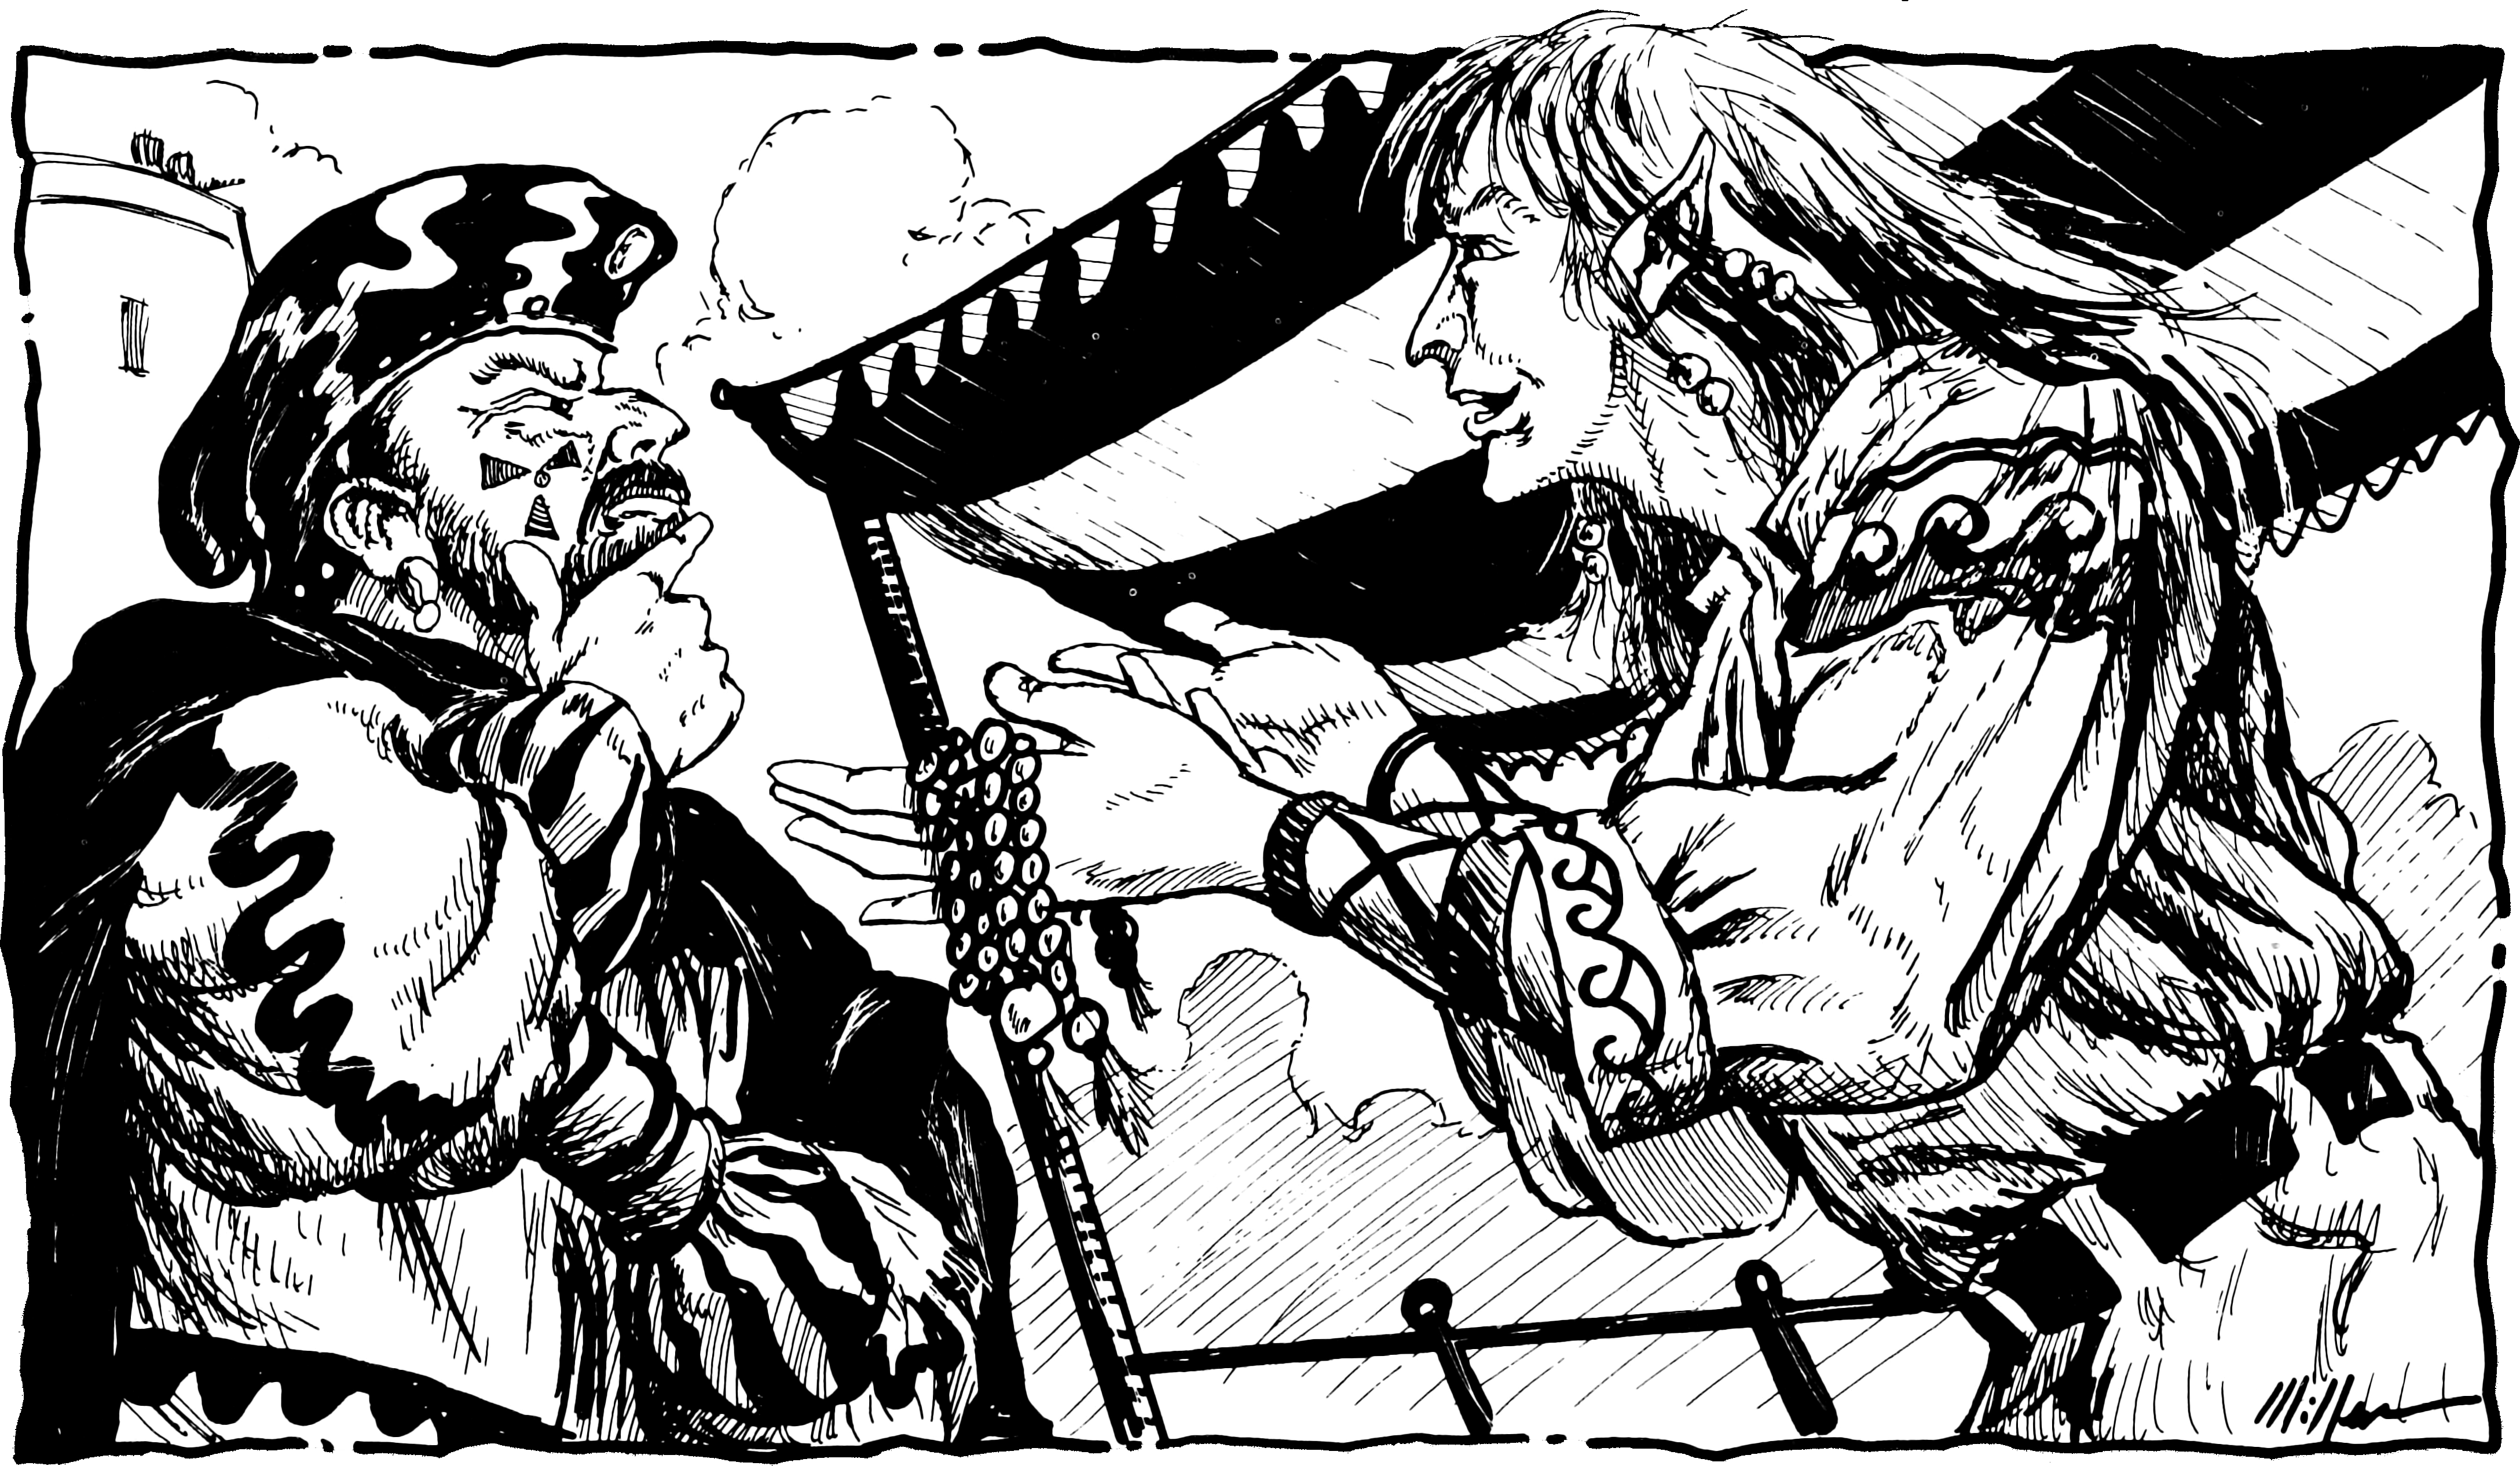
\includegraphics[width=\textwidth]{images/merchant-1.png}
\par\textit{\small\textcopyright Wizards of the Coast, 2020.}
\end{figure*}

\subsection{Adventuring Gear}

\Table{Adventuring Gear}{l RRRR}{
&& \multicolumn{3}{c}{\tableheader Weight}\\
\cmidrule[0.5pt]{3-5}
\tableheader Goods & \tableheader Cost & \tableheader M & \tableheader S & \tableheader L\\
Backpack (empty) & 2 cp & 1 kg & 0.25 kg & 4 kg\\
Barrel (empty) & 2 cp & 15 kg & &\\
Basket (empty) & 4 bits & 0.5 kg & &\\
Bedroll & 1 bits & 2.5 kg & 2.5 kg & 2.5 kg\\
Bell & 1 cp & & &\\
Blanket, winter & 5 bits & 1.5 kg & 0.37 kg & 6 kg\\
Block and tackle & 5 cp & 2.5 kg & &\\
Bottle, wine, glass & 2 cp & & &\\
Bucket (empty) & 5 bits & 1 kg & &\\
Caltrops & 1 cp & 1 kg & &\\
Candle & 1 bd & & &\\
Canvas (sq. m.) & 1 bits & 0.5 kg & &\\
Case, map or scroll & 1 cp & 0.25 kg & &\\
Chain (3 m.) & 30 cp & 1 kg & &\\
Chalk, 1 piece & 1 bd & & &\\
Chest (empty) & 2 cp & 12.5 kg & &\\
Crowbar & 2 cp & 2.5 kg & &\\
Firewood (per day) & 1 bd & 10 kg & &\\
Fishhook & 1 bits & & &\\
Fishing net, 2 sq. m. & 4 cp & 2.5 kg & &\\
Flask (empty) & 3 bd & 0.75 kg & &\\
Flint and steel & 1 cp & & &\\
Grappling hook & 1 cp & 2 kg & &\\
Hammer & 5 bits & 1 kg & &\\
Ink (30 ml vial) & 8 cp & & &\\
Inkpen & 1 bits & & &\\
Jug, clay & 3 bd & 9 lb. & &\\
Ladder, 3-meter & 5 bd & 10 kg & &\\
Lamp, common & 1 bits & 0.5 kg & &\\
Lantern, bullseye & 12 cp & 1.5 kg & &\\
Lantern, hooded & 7 cp & 1 kg & &\\
Lock (very simple) & 20 cp & 0.5 kg & &\\
Lock (average) & 40 cp & 0.5 kg & &\\
Lock (good) & 80 cp & 0.5 kg & &\\
Lock (amazing) & 150 cp & 0.5 kg & &\\
Manacles & 15 cp & 1 kg & &\\
Manacles, masterwork & 50 cp & 1 kg & &\\
Mirror, small steel & 10 cp & 0.25 kg & &\\
Mug/Tankard, clay & 2 bd & 0.5 kg & &\\
Oil (500 ml flask) & 1 bits & 0.5 kg & &\\
Paper (sheet) & 4 bits & & &\\
Parchment (sheet) & 2 bits & & &\\
Pick, miner's & 3 cp & 5 kg & &\\
Pitcher, clay & 2 bd & 2.5 kg & &\\
Piton & 1 bits & 0.25 kg & &\\
Pole, 3-meter & 2 bits & 4 kg & &\\
Pot, iron & 5 bits & 5 kg & &\\
Pouch, belt (empty) & 1 cp & 0.25 kg & 0.06 kg & 1 kg\\
Ram, portable & 10 cp & 10 kg & &\\
Rations, trail (per day) & 5 bits & 0.5 kg & 0.12 kg & 2 kg\\
Rope, giant hair (15 m.) & 50 cp & 5 kg & &\\
Rope, hempen (15 m.) & 1 cp & 5 kg & &\\
Rope, silk (15 m.) & 10 cp & 2.5 kg & &\\
Sack (empty) & 1 bits & 0.25 kg & 0.06 kg & 1 kg\\
Sealing wax & 1 cp & 0.5 kg & &\\
Sewing needle & 5 bits & & &\\
Signal whistle & 8 bits & & &\\
Signet ring & 5 cp & & &\\
Sledge & 1 cp & 5 kg & &\\
Soap (per 0.5 kg) & 5 bits & 0.5 kg & &\\
Spade or shovel & 2 cp & 4 kg & &\\
Spyglass & 1,000 cp & 0.5 kg & &\\
Tent & 10 cp & 10 kg & 2.5 kg & 40 kg\\
Torch & 1 bd & 0.5 kg & &\\
Vial, ink or potion & 1 cp & 0.05 kg & &\\
Waterskin & 1 cp & 2 kg & 0.5 kg & 8 kg\\
Whetstone & 2 bd & 0.5 kg & &\\
}


Some items weight differently for Small or Large characters, these items weigh one-quarter of the Medium-sized when made for Small characters and weigh four times as much the normal weight when made for Large characters. Containers for Small characters also carry one-quarter the normal amount, while containers for Large characters carry four times as much the normal amount.

A few of the pieces of adventuring gear are described below, along with any special benefits they confer on the user (``you'').


\textbf{Caltrops:} A caltrop is a four-pronged iron spike crafted so that one prong faces up no matter how the caltrop comes to rest. You scatter caltrops on the ground in the hope that your enemies step on them or are at least forced to slow down to avoid them. One 1-kilogram bag of caltrops covers an area 1.5 meter square.

Each time a creature moves into an area covered by caltrops (or spends a round fighting while standing in such an area), it might step on one. The caltrops make an attack roll (base attack bonus +0) against the creature. For this attack, the creature's shield, armor, and deflection bonuses do not count. If the creature is wearing shoes or other footwear, it gets a +2 armor bonus to AC. If the caltrops succeed on the attack, the creature has stepped on one. The caltrop deals 1 point of damage, and the creature's speed is reduced by one-half because its foot is wounded. This movement penalty lasts for 24 hours, or until the creature is successfully treated with a DC 15 \skill{Heal} check, or until it receives at least 1 point of magical curing. A charging or running creature must immediately stop if it steps on a caltrop. Any creature moving at half speed or slower can pick its way through a bed of caltrops with no trouble.

Caltrops may not be effective against unusual opponents.

\textbf{Candle:} A candle dimly illuminates a 1.5-meter radius and burns for 1 hour.

\textbf{Chain:} Chain has hardness 10 and 5 hit points. It can be burst with a DC 26 Strength check.

\textbf{Crowbar:} A crowbar grants a +2 circumstance bonus on Strength checks made for such purposes. If used in combat, treat a crowbar as a one-handed improvised weapon that deals bludgeoning damage equal to that of a club of its size.

\textbf{Flint and Steel:} Lighting a torch with flint and steel is a full-round action, and lighting any other fire with them takes at least that long.

\textbf{Grappling Hook:} Throwing a grappling hook successfully requires a \skill{Use Rope} check (DC 10, +2 per 3 meters of distance thrown).

\textbf{Hammer:} If a hammer is used in combat, treat it as a one-handed improvised weapon that deals bludgeoning damage equal to that of a spiked gauntlet of its size.

\textbf{Ink:} This is black ink. You can buy ink in other colors, but it costs twice as much.

\textbf{Jug, Clay:} This basic ceramic jug is fitted with a stopper and holds 4 liters of liquid.

\textbf{Lamp, Common:} A lamp clearly illuminates a 4.5-meter radius, provides shadowy illumination out to a 9-meter radius, and burns for 6 hours on 500 ml of oil. You can carry a lamp in one hand.

\textbf{Lantern, Bullseye:} A bullseye lantern provides clear illumination in a 18-meter cone and shadowy illumination in a 36-meter cone. It burns for 6 hours on 500 ml of oil. You can carry a bullseye lantern in one hand.

\textbf{Lantern, Hooded:} A hooded lantern clearly illuminates a 9-meter radius and provides shadowy illumination in a 18-meter radius. It burns for 6 hours on 500 ml of oil. You can carry a hooded lantern in one hand.

\textbf{Lock:} The DC to open a lock with the \skill{Open Lock} skill depends on the lock's quality: simple (DC 20), average (DC 25), good (DC 30), or superior (DC 40).

\textbf{Manacles and Manacles, Masterwork:} Manacles can bind a Medium creature. A manacled creature can use the \skill{Escape Artist} skill to slip free (DC 30, or DC 35 for masterwork manacles). Breaking the manacles requires a Strength check (DC 26, or DC 28 for masterwork manacles). Manacles have hardness 10 and 10 hit points.

Most manacles have locks; add the cost of the lock you want to the cost of the manacles.

For the same cost, you can buy manacles for a Small creature.

For a Large creature, manacles cost ten times the indicated amount, and for a Huge creature, one hundred times this amount. Gargantuan, Colossal, Tiny, Diminutive, and Fine creatures can be held only by specially made manacles.

\textbf{Oil:} A pint of oil burns for 6 hours in a lantern. You can use a flask of oil as a splash weapon. Use the rules for alchemist's fire, except that it takes a full round action to prepare a flask with a fuse. Once it is thrown, there is a 50\% chance of the flask igniting successfully.

You can pour a pint of oil on the ground to cover an area 1.5 meter square, provided that the surface is smooth. If lit, the oil burns for 2 rounds and deals 1d3 points of fire damage to each creature in the area.

\textbf{Ram, Portable:} This iron-shod wooden beam gives you a +2 circumstance bonus on Strength checks made to break open a door and it allows a second person to help you without having to roll, increasing your bonus by 2.

\textbf{Rope, Giant Hair:} This rope has 5 hardness, 2 hit points and can be burst with a DC 30 Strength check.

\textbf{Rope, Hempen:} This rope has 2 hit points and can be burst with a DC 23 Strength check.

\textbf{Rope, Silk:} This rope has 4 hit points and can be burst with a DC 24 Strength check. It is so supple that it provides a +2 circumstance bonus on \skill{Use Rope} checks.

\textbf{Spyglass:} Objects viewed through a spyglass are magnified to twice their size.

\textbf{Torch:} A torch burns for 1 hour, clearly illuminating a 6-meter radius and providing shadowy illumination out to a 12-meter radius. If a torch is used in combat, treat it as a one-handed improvised weapon that deals bludgeoning damage equal to that of a gauntlet of its size, plus 1 point of fire damage.

\textbf{Vial:} A vial holds 30 milliliters of liquid. The stoppered container usually is no more than 3 centimeters wide and 8 centimeters high.

\subsection{Special Substances And Items}
The following items are often, but not always available for sale in the Bard's Quarter of most city-states. Contacting someone willing to sell these and other associated goods usually requires proficient use of the \skill{Bluff}, \skill{Diplomacy}, and/or \skill{Gather Information} skills.

Any of these substances except for the everburning torch and holy water can be made by a character with the \skill{Craft} (alchemy) skill.

\ItemTable{Special Substances and Items}{
Acid (flask) & 10 cp & 0.5 kg\\
Alchemist's fire (flask) & 20 cp & 0.5 kg\\
Antitoxin (vial) & 50 cp &\\
Balican sting & 5 cp & 0.5 kg\\
Chitin ointment & 40 cp & 0.5 kg\\
Draxia ointment & 20 cp & 0.5 kg\\
Esperweed & 250 cp &\\
Everburning torch & 110 cp & 0.5 kg\\
Holy water (flask) & 25 cp & 0.5 kg\\
Hypnotic brew & 30 cp & 0.5 kg\\
Ignan tallgrass & 100 cp &\\
Kuzza powder & 20 cp &\\
Ranike sap (1 liter) & 2 cp & 0.5 kg\\
Smokestick & 20 cp & 0.25 kg\\
\TableSubheader{Splash-globe}&&\\
~ Acid & 10 cp &\\
~ Kip pheromones & 30 cp &\\
~ Liquid darkness & 10 cp &\\
~ Liquid dust & 10 cp &\\
~ Liquid fire & 10 cp &\\
~ Liquid light & 10 cp &\\
~ Poison & Poison cost $\times$ 1.5 &\\
~ Ranike sap smoke & 10 cp &\\
~ Stench cloud & 50 cp &\\
~ Stun cloud & 35 cp &\\
Sunrod & 2 cp & 0.5 kg\\
Tanglefoot bag & 50 cp & 2 kg\\
Thunderstone & 30 cp & 0.5 kg\\
Tindertwig & 1 cp &\\
}

\textbf{Acid:} You can throw a flask of acid as a splash weapon. Treat this attack as a ranged touch attack with a range increment of 3 meters. A direct hit deals 1d6 points of acid damage. Every creature within 1.5 meter of the point where the acid hits takes 1 point of acid damage from the splash.

\textbf{Alchemist's Fire:} You can throw a flask of alchemist's fire as a splash weapon. Treat this attack as a ranged touch attack with a range increment of 3 meters.

A direct hit deals 1d6 points of fire damage. Every creature within 1.5 meter of the point where the flask hits takes 1 point of fire damage from the splash. On the round following a direct hit, the target takes an additional 1d6 points of damage. If desired, the target can use a full-round action to attempt to extinguish the flames before taking this additional damage. Extinguishing the flames requires a DC 15 Reflex save. Rolling on the ground provides the target advantage on the save. Leaping into a lake or magically extinguishing the flames automatically smothers the fire.

\textbf{Antitoxin:} If you drink antitoxin, you get a +5 alchemical bonus on Fortitude saving throws against poison for 1 hour.

\textbf{Balican Sting:} This mixture of many vegetal irritants is used in conjunction with the flint-tipped javelin of the Balican fleet. Bards working for the late king Andropinis developed the substance to improve the damage done by his warriors fighting against the thick-skinned giants. This mixture, which is only effective against giants of the beasthead, crag, desert, or plains variety, causes the wound made by a balican javelin that breaks within it to itch. Unless a DC 15 Wisdom check is made by the giant on each of the following 1d4 rounds, he will scratch and inadvertently rub the shallow shards deeper, causing an additional 1d4 points of damage for each failed check.

\textbf{Chitin Ointment:} This salve is used to cure damaged chitin on kreens and other insectoid creatures. Once applied, as a standard action, this substance mends brittle or broken chitin, effectively stabilizing the creature if it had less than 0 hit points. Applying this substance to non-chitinous creatures produces no effects.

\textbf{Draxia Ointment:} The draxia weed grows on the islands of the Sea of Silt. It can be turned into an ointment that repels silt spawn by mixing the plant's juices with oil or fat. The ointment, when applied to the skin, emits a smell that repels silt spawn for two hours. Silt spawn will not come within 3 meters of a creature or object coated with draxia ointment. Although adult silt horrors find the smell irritating, they are usually unaffected by it. Sometimes silt horrors are irritated to such a level, however, that they may attack the creature or object giving off the smell. There is a 60\% chance that a silt horror will ignore all other targets and instead attack a character or object that smells of draxia weed.

\textbf{Everburning Torch:} This otherwise normal torch has a continual flame spell cast upon it. An everburning torch clearly illuminates a 6-meter radius and provides shadowy illumination out to a 12-meter radius.

\textbf{Holy Water:} Holy water damages undead creatures and evil outsiders almost as if it were acid. A flask of holy water can be thrown as a splash weapon.

Treat this attack as a ranged touch attack with a range increment of 3 meters. A flask breaks if thrown against the body of a corporeal creature, but to use it against an incorporeal creature, you must open the flask and pour the holy water out onto the target. Thus, you can douse an incorporeal creature with holy water only if you are adjacent to it. Doing so is a ranged touch attack that does not provoke attacks of opportunity.

A direct hit by a flask of holy water deals 2d4 points of damage to an undead creature or an evil outsider. Each such creature within 1.5 meter of the point where the flask hits takes 1 point of damage from the splash.

Temples to good deities sell holy water at cost (making no profit).

\textbf{Ignan Tallgrass:} A redish plant that grows in the Burning Plains near the Last Sea, ignan tallgrass can be harvested from the plains after flashfires, when they are easily spotted in small clumps untouched by the fires. Ignan tallgrass is tough and can be used to make mats and roofs of twinned fibers that stay fireproof for several months, if the harvesters are brave enough to face the flashfires to get to it, as the plant cannot be cultivated. If ignan tallgrass is sun-dried, crushed, and ingested within a week of it being picked, unless somehow magically kept fresh (as through the nurturing seeds spell), it confers resistance to fire 1 for one hour.

\textbf{Kuzza Powder:} Kuzza peppers are very hot. Typically, these vivid red peppers, when ripe, measure 2 to 2 1/2 inches long. These peppers are sometimes dried and ground into a powder by unscrupulous gladiators who use a blowpipe to blow the powder on a target, causing sever irritation. Treat this blowpipe as a blowgun with half the range increment. Filling a blowpipe is a move action that provokes attacks of opportunity. A direct hit blinds a creature for 1 round unless it makes a Fortitude save (DC 15). Every creature within 1.5 meter of the target takes a $-2$ penalty to \skill{Search} and \skill{Spot} checks for 5 rounds.

\textbf{Ranike Sap:} The sap of the ranike tree, which constantly runs down its bark, is toxic to insects. Gulg posesses the secret of safely extracting large quantities of sap from this tree, effectively milking the tree in a process called ``bleeding''. If a liter of the sap is poured in a large receptacle, such as a brazier, and lit afire, a clear smoke that impairs neither vision or breathing forms, filling a 15-meter cube (a moderate or stronger wind dissipates the smoke in 5 rounds). The smoke repels mundane insects, while giant insects, or those creatures that can be categorised as insect-like (such as antloids, kanks, and thri-kreen), that breathe or contact the smoke must make a Fortitude save (DC 15) each round for one minute; failure indicates that they are sickened for that round. The sap burns 1 hour for each liter of sap in the receptacle, after which the smoke dissipates naturally.

A shallow depression in the ground several meters wide can replace the need for a receptacle. The sap can also be used to deliniate an area---each liter poured on the ground can create a line a few inches wide and 3 meters long. When such a line is set afire, it burns for 1 minute and creates smoke in an area 3 meters long by 1.5 meter wide and high.

\textbf{Smokestick:} This alchemically treated wooden stick instantly creates thick, opaque smoke when ignited. The smoke fills a 3-meter cube (treat the effect as a fog cloud spell, except that a moderate or stronger wind dissipates the smoke in 1 round). The stick is consumed after 1 round, and the smoke dissipates naturally.

\textbf{Splash-globes:} Splash-globes are spherical glass jars containing contact poison or up to half a pint of some alchemical fluid. In addition to bursting on impact like any grenade, splash-globes can be placed in hinged pelota, thus giving the grenade additional range when fired through a splash-bow or dejada. The following types of splash-globes are available:

 \textit{Acid:} Standard flask acid can be placed in splash-globes.

 \textit{Contact Poison:} Any contact poison can be placed in a splash-globe.

 \textit{Kip Pheromones:} This splash-globe is commonly crafted by bards using kip pheromones collected by dwarven kip herders. The liquid contained within the globe is an alchemical mixture that turns into smoke on contact with air. The smoke produced is clear and does not impair vision or breathing, filling a 3-meter cube for one minute (a moderate or stronger wind dissipates the smoke in 1 round). Those within the smoke must make a DC 15 Fortitude save each round they are in contact with it or become fascinated for the as long as the smoke remains. Dwarves gain a +4 racial bonus on their Fortitude save against kip pheromones.

 \textit{Liquid Darkness:} Anyone struck directly by liquid darkness must make a Reflex save (DC 15) or be blinded for one minute. Those splashed with liquid darkness have their vision blurred for one minute if they fail a DC 15 Reflex save, granting their opponents concealment. In addition, all natural fires within the splash area are instantly extinguished. Liquid darkness immediately extinguishes liquid light.

 \textit{Liquid Dust:} The liquid from this splash-globe turns into dust on contact with the air. You can use this liquid to cover up to 20 1.5-meter squares of tracks. On impact, liquid dust forms a 4.5-meter diameter cloud, three meters high that lasts one round. Alternately, liquid dust can be launched via slash-globes. Anyone struck directly by liquid dust must make a DC 15 Fortitude save each round for one minute; failure dictates that they are nauseated for that round. Those splashed with liquid dust suffer the same effect for one round if they fail a DC 15 Fortitude save.

 \textit{Liquid Fire:} Alchemist's fire can be placed in splash-globes.

 \textit{Liquid Light:} This splash-globe contains two liquids that mix together when the splash-globe is ruptured. The resulting mixture glows for eight hours. If you break the liquid light globe while it is still in its pouch, the pouch can serve as a light source just like a sunrod. Anyone struck directly by liquid light must make a DC 20 Fortitude save or be temporarily dazzled ($-1$ on all attack rolls) for 1 minute, and will glow in darkness for eight hours unless they somehow cover the affected areas. Creatures splashed with liquid light (see grenade rules) also glow in the darkness, but are not blinded.

 \textit{Ranike Sap Smoke:} The liquid from this splash-globe is an alchemical mixture of ranike sap that turns into smoke on contact with air. The smoke produced is clear and does not impair vision or breathing, filling a 3-meter cube (a moderate or stronger wind dissipates the smoke at the end of the character's action). The smoke repels mundane insects, while giant insects, or those creatures that can be categorised as insect-like (such as antloids, kanks, and thri-kreens), that breath or enter in contact with the smoke must make a DC 15 Fortitude save each round for one minute; failure indicates that they are sickened for that round. This small quantity of sap only reacts with the air for 1 round, after which the smoke dissipates naturally.

 \textit{Stench Cloud:} The liquid inside this splash-globe is crafted from fordorran musk and stinkweed extract. The foul liquid turns into smoke on contact with air. The smoke produced is clear and does not impair vision or breathing, filling a 3-meter cube for one minute (a moderate or stronger wind dissipates the smoke in 1 round). Those within the smoke must make a DC 15 Fortitude save each round they are in contact with it or become nauseated for as long as they remain in contact with the cloud.

 \textit{Stun Cloud:} The liquid inside this splash-globe is crafted from boiled floater jelly combined with the pulped spines from a poisonous cactus. The liquid turns into smoke on contact with air. The smoke produced is clear and does not impair vision or breathing, filling a 3-meter cube for one minute (a moderate or stronger wind dissipates the smoke in 1 round). Those within the smoke must make a DC 15 Fortitude save each round they are in contact with it or become stunned for as long as they remain in contact with the cloud.

\textbf{Sunrod:} This 30-centimeter long, gold-tipped, iron rod glows brightly when struck. It clearly illuminates a 9-meter radius and provides shadowy illumination in a 18-meter radius. It glows for 6 hours, after which the gold tip is burned out and worthless.

\textbf{Tanglefoot Bag:} When you throw a tanglefoot bag at a creature (as a ranged touch attack with a range increment of 3 meters), the bag comes apart and the goo bursts out, entangling the target and then becoming tough and resilient upon exposure to air. An entangled creature takes a $-2$ penalty on attack rolls and a $-4$ penalty to Dexterity and must make a DC 15 Reflex save or be glued to the floor, unable to move. Even on a successful save, it can move only at half speed. Huge or larger creatures are unaffected by a tanglefoot bag. A flying creature is not stuck to the floor, but it must make a Reflex save (DC 15) or be unable to fly (assuming it uses its wings to fly) and fall to the ground. A tanglefoot bag does not function underwater.

A creature that is glued to the floor (or unable to fly) can break free by making a DC 17 Strength check or by dealing 15 points of damage to the goo with a slashing weapon. A creature trying to scrape goo off itself, or another creature assisting, does not need to make an attack roll; hitting the goo is automatic, after which the creature that hit makes a damage roll to see how much of the goo was scraped off. Once free, the creature can move (including flying) at half speed. A character capable of spellcasting who is bound by the goo must make a \skill{Concentration} check (DC 15) to cast a spell. The goo becomes brittle and fragile after 2d4 rounds, cracking apart and losing its effectiveness. An application of universal solvent to a stuck creature dissolves the alchemical goo immediately.

\textbf{Thunderstone:} You can throw this stone as a ranged attack with a range increment of 6 meters. When it strikes a hard surface (or is struck hard), it creates a deafening bang that is treated as a sonic attack. Each creature within a 3-meter-radius spread must make a DC 15 Fortitude save or be deafened for 1 hour. A deafened creature, in addition to the obvious effects, takes a $-4$ penalty on initiative and has a 20\% chance to miscast and lose any spell with a verbal component that it tries to cast.

Since you don't need to hit a specific target, you can simply aim at a particular 1.5-meter square. Treat the target square as AC 5.

\textbf{Tindertwig:} The alchemical substance on the end of this small, wooden stick ignites when struck against a rough surface. Creating a flame with a tindertwig is much faster than creating a flame with flint and steel (or a magnifying glass) and tinder. Lighting a torch with a tindertwig is a standard action (rather than a full-round action), and lighting any other fire with one is at least a standard action.
\subsectionA{Metaempiric Components}
Useful for spellcasters, these items are special material components that have a chance of influencing the casting of certain spells while held in hand. Since a metempiric component must be held in one hand to use, it cannot be used in conjunction with the \feat{Still Spell} feat and, being optional for the casting of a spell, does not count as a normal material component for the purpose of the \feat{Eschew Materials} feat. Metempiric components are consumed during the casting of a spell, unless otherwise noted.

\ItemTable{Metaempiric Components}{
Aviarag horn & 1,350 cp & 2.5 kg\\
Beasthead blood & 45 cp & 0.5 kg\\
Dagorran crystal, diminutive & 100 cp &\\
Dagorran crystal, tiny & 300 cp & 0.25 kg\\
Defiler's ash & 1,700 cp &\\
Defiled poisonweed petals & 350 cp &\\
Eagle beasthead feather & 40 cp &\\
Roc feather & 450 cp &\\
Royal justice token & 1,375 cp & 0.5 kg\\
Shadow giant fumes & 390 cp & 0.5 kg\\
Sun paraelemental essence & 935 cp & 0.5 kg\\
T'chowb's thalamus & 1,250 cp & 0.25 kg\\
}

\textbf{Aviarag Horn:} A horn willingly given by an aviarag for use by someone after its passing into death is a powerful weapon for those seeking to do good. When presented while casting a spell, the goodness still emanating from the beast's horn is so tangible that the spell itself benefits from it. When used as a component for any spell with the good descriptor, the aviarag horn increases the spell's effective caster level by 1d4. An aviarag horn is not consumed after being used.

\textbf{Beasthead Blood:} As sorcerous mutations of normal Athasian giants, the blood of beasthead giants has some magical properties. When beasthead blood is used as a component in any transmutation spell, it increases the spell's saving throw DC by +1. Inexplicably, only druids and preservers may use beasthead blood this way; it provides no benefit for other types of spellcasters.

\textbf{Dagorran Crystal:} This green crystal growth is extracted from the body of a daggoran. Daggorans come in two sizes, which affect the size and potency of the crystal: a Medium daggoran provides a Diminutive crystal while a Large daggoran provides a Tiny crystal. When used as a component for a spell with the mind-affecting descriptor, a Diminutive daggoran crystal increases the spell's saving throw DC by +2.

\textbf{Defiler's Ash:} Mixed in with a special mixture of blood, these ashes must be taken from at least three different spellcasters' ashen circles caused by powerful spellcasting (spell level 6th and above). When used in the casting of a spell with the necromancy descriptor, defiler's ash empower the spell as if the caster had applied the Empower Spell feat (but without changing the spell's effective level or increasing its casting time).

\textbf{Defiled Poisonweed Petals:} The bright orange petals of a poisonweed plant turned undead by the action of defiling represent the epitome of noxiousness. When used as a component for any spell with the death descriptor, the petals of a defiled poisonweed increase the spell's saving throw DC by +2.

\textbf{Eagle Beasthead Feather:} If a feather from an eagle-headed beasthead giant is in hand when falling, it can be used as a component when casting feather fall, doubling the duration of the spell.

\textbf{Roc Feather:} These huge feathers---from anywhere between 0.6 and 1.2 meter long---come from an Athasian rock. When used as a component for a spell confering flight, a roc feather doubles the spell's duration.

\textbf{Royal Justice Token:} Only used by templars in the service of the sorcerer-monarch for which the token was created, the royal justice token shows graven symbols associated with the justice system used in a particular city-state. Symbols include ever-vigilant eyes, readied swords, and open hand or closed fist. When used as a component for the \spell{wrath of the sorcerer-king} spell, the token increases the spell's effective caster level by +2. A royal justice token is not consumed after being used.

\textbf{Shadow Giant Fumes:} If bottled, the black, cold fumes that emanate from a shadow giant's mouth as it speaks can be used to enhance spells that have a connection to the Black. When used as a component for the spells \spell{greater shadow conjuration}, \spell{shades}, or \spell{shadow conjuration}, the potency of the spell is one-fifth (20\%) better than normal.

\textbf{Sun Paraelemental Essence:} This bright and blinding essence comes from a dead sun paraelemental of at least Huge size. The essence must be trapped in a clear crystal container within one minute of the elemental's death and must always be kept under the light of the sun during the day, or else losing its potency. During the night, the light fades and gives off the same illumination as a candle. When used as a component for any spell with the light descriptor, the essence increases the effective caster level by +2.

\textbf{T'chowb's Thalamus:} The thalamus of a recently fed (within the last 24 hours) t'chowb is said to be seething with absorbed intelligence. When used as a metempiric component, the t'chowb's thalamus gives the caster a +10 circumstance bonus on caster level checks made to overcome a target's spell resistance.
\subsection{Psychoactive Components}
Useful for manifesters, these items are components that have a chance of influencing the manifestation of certain powers when used properly. Unlike metempiric components, each psychoactive component must be used in a specific fashion in order to provide its benefits to the manifester. Unless otherwise noted, psychoactive components are consumed during the manifesting of a power.

Also included in this category is a creature sometimes used by psionic characters to access the residual psionic energy their mind's produce throughout the day.

\ItemTable{Psychoactive Components}{
Aviarag horn melange & 250 cp & 0.5 kg\\
Bouyan crystal & 400 cp & 1 kg\\
Cilops compound eye & 65 cp & \\
Dagorran crystal, diminutive & 100 cp & \\
Dagorran crystal, tiny & 300 cp & \onequarter kg\\
Tas'l worm & 100 cp & \\
T'chowb's thalamus & 1,250 cp & \onequarter kg\\
}

\textbf{Aviarag Horn Melange:} The great horn of the noble aviarag, when crushed and mixed with a specially treated wine, preserves some of the psionic power of the aviarag and can expand the reach and power of the drinker's mind. A manifester drinking this psychoactive substance no more than 1 minute before using the \psionic{mindwipe} power increases the power's save DC by +2, and drinking it before manifesting \psionic{mindlink} doubles the power's range, as per the \feat{Enlarge Power} feat (but without changing the power's effective level or requiring the expendature of a psionic focus). Drinking this melange is a standard action that provokes attacks of opportunity.

\textbf{Bouyan Crystal:} From salt formations found within the great salt plains, the clear gray bouyan stone is cut to a great degree of perfection, allowing a manifester to focus his mind upon it. A manifester that concentrates upon a held bouyan crystal when manifesting any telepathy power (a free action, assuming the manifester is already holding the component) increases the power's effective manifester level by +1.

\textbf{Cilops Compound Eye:} Crushing the central compound eye of a cilops produces a thick jelly that may extend the user's senses of his surroundings. If this jelly is spread over the eyes of a character (a full-round action) before he manifests object reading, and the temporary blindness it induces is endured for the extent of the power's duration, then this power always successfully identifies all other former owners of an object in sequence, with no chance that former owners will be skipped and thus not identified. Removing the jelly from one's eyes, thus negating the blindness, takes 1 minute. Eating the jelly before manifesting sensitivity to psychic impressions reduces the manifesting time of that power to 10 minutes.

\textbf{Dagorran Crystal:} This green crystal growth is extracted from the body of a daggoran. Manifesters use these crystals to harness the dagorran's ability to sense the psionic nature of creatures. A Diminutive daggoran crystal gives manifesters advantage to \skill{Psicraft} checks made when using the \psionic{psychic tracking} psionic power, while a Tiny daggoran crystal gives a +5 competence bonus. Such a crystal is not consumed when used.

\textbf{Tas'l Worm:} Tas'l worms are worms of Diminutive size, similar in appearance to ock'n, but without eyestalks. Only found on living psionic creatures, these 1-inch long worms snake slowly between the skin and the skull of their host, accumulating and living off of residual psionic energy.

A tas'l worm can be removed by cutting open the skin. A character can remove a worm by taking 10 minutes to locate and extract it from the host's scalp. The extraction does 1d6 points of damage to the victim, and has a 75\% chance of killing the worm in the process. If a successful \skill{Heal} check (DC 20) is made, the cutting damage is reduced to 1d2, with no chance of killing the worm.

A worm outside of its host lives for 1 hour. The worm, when put against the skin of a psionic creature, burrows into its flesh, causing 1 point of damage. Afterwards, the worm must stay within the host for at least 24 hours before it amasses enough residual energy to be used. Tas'l worms use the innocuous vermin statistics (see page 191 of Terrors of Athas). A worm linked to a host has a lifespan of 2d6 months. If more than one worm live on the same scalp, there is a 55\% chance for 1d2 worms to spawn each month thereafter.

The creature hosting tas'l worms can make a \skill{Concentration} check (DC 20) as a free action, once per day, to tap the energy they contain. If the check is successful, each tas'l worm hosted by a creature provides 1 power point. All worms must be tapped at once, or none at all. These power points are considered a part of the creature's own power point reserve for the purpose of using stored power points. A failed check can be retried on the character's next turn.

The hosting creature receives a cumulative $-1$ circumstance penalty to Will saves against telepathic powers for each worm living within its body, as the worms make their host more responsive to outside psionic influence.

A tas'l worm registers as psionic to \psionic{detect psionics}.

\textbf{T'chowb's Thalamus:} The thalamus of a recently fed (within the last 24 hours) t'chowb is said to be seething with absorbed intelligence. If crushed in one's hand during the manifestation of a power (a free action, assuming the manifester is already holding the component), the t'chowb's thalamus gives a manifester a +10 circumstance bonus on manifester level checks made to overcome a target's power resistance.
\subsectionA{Tools and Skill Kits}

\ItemTable{Tools and Skill Kits}{
Alchemist's lab & 500 cp & 20 kg\\
Artisan's tools & 5 cp & 2.5 kg\\
Artisan's tools, masterwork & 55 cp & 2.5 kg\\
Book of poisons & 125 cp & 1 kg\\
Candle of rejuvenation & 50 cp & \\
Climber's kit & 80 cp & 2.5 kg1\\
Concealing weave & 5 cp & 1 kg\\
Disguise kit & 50 cp & 4 kg1\\
Healer's kit & 50 cp & 0.5 kg\\
Holly and mistletoe & & \\
Holy symbol, silver & 25 cp & 0.5 kg\\
Holy symbol, wooden & 1 cp & \\
Hourglass & 25 cp & 0.5 kg\\
Magnifying glass & 100 cp & \\
Meditative kit & 35 cp & 1.5 kg\\
Musical instrument, common & 5 cp & 1.5 kg1\\
Musical instrument, masterwork & 100 cp & 1.5 kg1\\
Navigator kit & 75 cp & 5 kg\\
Remote viewing kit & & 5 kg\\
Scale, merchant's & 2 cp & 0.5 kg\\
Spell component pouch & 5 cp & 1 kg\\
Spellbook, wizard's (blank) & 15 cp & 1.5 kg\\
Thieves' tools & 30 cp & 0.5 kg\\
Thieves' tools, masterwork & 100 cp & 1 kg\\
Tool, masterwork & 50 cp & 0.5 kg\\
Water clock & 1,000 cp & 100 kg\\
}

The items described below are particularly useful to characters that have certain specific skills or abilities and are used in specific situations.


\textbf{Alchemist's Lab:} An alchemist's lab always has the perfect tool for making alchemical items, so it provides +2 circumstance bonus on \skill{Craft} (alchemy) checks. It has no bearing on the costs related to the \skill{Craft} (alchemy) skill. Without this lab, a character with the \skill{Craft} (alchemy) skill is assumed to have enough tools to use the skill but not enough to get the +2 bonus that the lab provides.

\textbf{Artisan's Tools, Masterwork:} These tools serve the same purpose as artisan's tools (above), but masterwork artisan's tools are the perfect tools for the job, so you get +2 circumstance bonus on \skill{Craft} checks made with them.

\textbf{Artisan's Tools:} These special tools include the items needed to pursue any craft. Without them, you have to use improvised tools (-2 penalty on \skill{Craft} checks), if you can do the job at all.

\textbf{Book of Poisons:} The original Book of Poisons is rumored to have been written by the half-elven bard Cabal, with current copies containing but fragments of the original poison recipes. This set of clay tablets is covered with markings, known mostly to bards, that can only be understood by making a \skill{Decipher Script} check (DC 15). Once deciphered, the reader can see that they contain a number of recipes that describe, step-by-step, tried-and-true methods for crafting specific poisons. The tablets grant the following benefits when used in conjunction with the crafting of poisons described in the set (normally 5 to 10 different poisons, of the DM's choice): +2 circumstance bonus to \skill{Craft} (poisonmaking) checks and a +1 to the save DC of the poisons being crafted. This last bonus stacks with the scorpion's touch bardic ability.

\textbf{Candle of Rejuvenation:} This item allows a manifester to recover power points as if he were resting at night. The manifester recovers 10 power points at the end of each complete hour spent within 3 meters of a lit candle. By making an \skill{Autohypnosis} DC 15 check, this amount increases by one-half. Each candle burns for a total of eight hours.

\textbf{Climber's Kit:} This is the perfect tool for climbing and gives you +2 circumstance bonus on \skill{Climb} checks.

\textbf{Concealing Weave:} This kit is composed of one or more related articles of clothing specifically made to camouflage a caster's arm and hand movements while casting a spell. This kit grants +2 circumstance bonus on \skill{Bluff} checks made to conceal the casting of spells with a somatic component.

\textbf{Disguise Kit:} The kit is the perfect tool for disguise and provides +2 circumstance bonus on \skill{Disguise} checks. A disguise kit is exhausted after ten uses.

\textbf{Healer's Kit:} It is the perfect tool for healing and provides +2 circumstance bonus on \skill{Heal} checks. A healer's kit is exhausted after ten uses.

\textbf{Holy Symbol, Silver or Wooden:} A holy symbol focuses positive energy. A cleric uses it as the focus for his spells and as a tool for turning undead. Each religion has its own holy symbol.

 \textit{Unholy Symbols:} An unholy symbol is like a holy symbol except that it focuses negative energy and is used by evil clerics (or by neutral clerics who want to cast evil spells or command undead).

 \textit{Sorcerer-king's Sigil:} A sorcerer-king's sigil is like a holy symbol for templars. It is the sign of their rank and station within the templarate. It is unique to each city-state.

\textbf{Magnifying Glass:} This simple lens allows a closer look at small objects. It is also useful as a substitute for flint and steel when starting fires. Lighting a fire with a magnifying glass requires light as bright as sunlight to focus, tinder to ignite, and at least a full-round action. A magnifying glass grants +2 circumstance bonus on \skill{Appraise} checks involving any item that is small or highly detailed.

\textbf{Meditative Kit:} This small and delicately carved crystal container produces an hypnotic rainbow-like effect while filled with clear water and struck by light. After 1 minute of uninterrupted observation of the rainbow pattern, the kit provides +2 circumstance bonus to the next \skill{Autohypnosis} check made by the viewer within the next 10 minutes.

\textbf{Musical Instrument, Common or Masterwork:} A masterwork instrument grants +2 circumstance bonus on \skill{Perform} checks involving its use.

\textbf{Navigator's Kit:} Prized posessions of many trading houses and frequent wanderers of the wastes, each of these kits is composed of a set of maps made of straight sticks representing roads, and small stones for villages, cities and others special locations, all lashed together by strings. If you succeed at a \skill{Knowledge} (geography) check DC 10 while using this kit, you gain a +4 bonus on \skill{Survival} checks made to keep from getting lost.

\textbf{Remote Viewing Kit:} This kit allows for a more potent use of the \psionic{remote viewing} power. Unlike other class or skill kits, this kit is created from local natural materials, effectively making it free in cost, but its user must recreate the kit before each use. Five ranks in \skill{Knowledge} (psionics), and 10 minutes, are required to create the kit. It must be created in silence, without distractions, and in a windless area. The kit takes the form of a 1.5-meter square patch of flat ground, covered with sand or particulate dirt to a depth of at least 2.5 centimeters, with 1d6 palm-sized stones deposited on it. Lines and circles are then traced around the stones and over the entire surface, creating a unique, maze-like pattern.

To gain the benefits of the kit, the user must focus on the patch of ground and succeed at a DC 15 \skill{Concentration} check after its creation; failure indicating that the user needs to recreate the kit anew. A successful check means the user's next manifestation of remove viewing, which must be within 1 minute of making the check, is altered in the following ways. First, the subject of the user's viewing attempt receives a $-2$ penalty to his Will saving throw against the \psionic{remote viewing}. Second, the user receives +2 circumstance bonus to \skill{Concentration} checks made to manifest a power through \psionic{remote viewing}. Finally, the user receives +2 circumstance bonus to \skill{Hide} checks to prevent his quasi-real viewpoint from being noticed by the subject he his viewing.

The effects of this kit can be made more potent if more than one character assists with its creation. Each character that helps adds another 1.5-meter square to the space taken by the kit, and another 10 minutes to the time required for the kit's completion. Each character that succeeds at a DC 15 \skill{Concentration} check at the time of the kit's completion can use the aid another action to help the user with skill checks made while the user is manifesting \psionic{remote viewing}. A kit created in this fashion is more complex, and as such requires two more ranks in \skill{Knowledge} (psionics) to create for each additional character that helped in its creation. Only a limited number of characters can help to create a remove viewing kit, equal to half the user's manifester level.

\textbf{Scale, Merchant's:} A scale grants +2 circumstance bonus on \skill{Appraise} checks involving items that are valued by weight, including anything made of precious metals.

\textbf{Spell Component Pouch:} A spellcaster with a spell component pouch is assumed to have all the material components and focuses needed for spellcasting, except for those components that have a specific cost, divine focuses, and focuses that wouldn't fit in a pouch.

\textbf{Spellbook, Wizard's (Blank):} A spellbook has 100 pages of parchment, and each spell takes up one page per spell level (one page each for 0-level spells).

\textbf{Thieves' Tools, Masterwork:} This kit contains extra tools and tools of better make, which grant +2 circumstance bonus on \skill{Disable Device} and \skill{Open Lock} checks.

\textbf{Thieves' Tools:} This kit contains the tools you need to use the \skill{Disable Device} and \skill{Open Lock} skills. Without these tools, you must improvise tools, and you have disadvantage on \skill{Disable Device} and \skill{Open Lock} checks.

\textbf{Tool, Masterwork:} This well-made item is the perfect tool for the job. It grants +2 circumstance bonus on a related skill check (if any). Bonuses provided by multiple masterwork items used toward the same skill check do not stack.

\textbf{Water Clock:} This large, bulky contrivance gives the time accurate to within half an hour per day since it was last set. It requires a source of water, and it must be kept still because it marks time by the regulated flow of droplets of water.
\subsection{Clothing}
Clothes weigh one-quarter the normal amount when made for Small characters, and four times as much when made for Large characters.

\Table{Clothing}{lRRRR}{
&& \multicolumn{3}{c}{\tableheader Weight}\\
\cmidrule[0.25pt]{3-5}
\tableheader Item & \tableheader Cost & \tableheader S & \tableheader M & \tableheader L\\
Artisan's outfit & 1 cp & 0.5 kg & 2 kg & 8 kg\\
Cleric's vestments & 5 cp & 0.75 kg & 3 kg & 12 kg\\
% Cold weather outfit & 8 cp & 3.5 kg & 3.5 kg & 15 kg\\
Courtier's outfit & 30 cp & 0.75 kg & 3 kg & 12 kg\\
Elven outfit & 30 cp & 0.62 kg & 2.5 kg & 10 kg\\
Entertainer's outfit & 3 cp & 0.5 kg & 2 kg & 8 kg\\
Explorer's outfit & 10 cp & 1 kg & 4 kg & 16 kg\\
High templar's outfit & 100 cp & 0.62 kg & 2.5 kg & 10 kg\\
% Monk's outfit & 5 cp & 1 kg & 1 kg & 1 kg\\
Noble's outfit & 75 cp & 1.25 kg & 5 kg & 20 kg\\
Peasant's outfit & 1 sp & 0.25 kg & 1 kg & 4 kg\\
Royal defiler's outfit & 80 cp & 0.62 kg & 2.5 kg & 10 kg\\
Royal outfit & 200 cp & 1.87 kg & 7.5 kg & 30 kg\\
Scholar's outfit & 5 cp & 0.75 kg & 3 kg & 12 kg\\
Slave's outfit & 2 bd & 0.12 kg & 0.5 kg & 2 kg\\
Traveler's outfit & 1 cp & 0.62 kg & 2.5 kg & 10 kg\\
Wastelander outfit & 20 cp & 0.75 kg & 3 kg & 12 kg\\
}


\textbf{Artisan's Outfit:} This outfit includes a shirt with buttons, a skirt or pants with a drawstring, shoes, and perhaps a cap or hat. It may also include a belt or a leather or cloth apron for carrying tools.

\textbf{Cleric's Vestments:} These ecclesiastical clothes are for performing priestly functions, not for adventuring.

% \textbf{Cold Weather Outfit:} A cold weather outfit includes a wool coat, linen shirt, wool cap, heavy cloak, thick pants or skirt, and boots. This outfit grants a +5 circumstance bonus on Fortitude saving throws against exposure to cold weather.

\textbf{Courtier's Outfit:} This outfit includes fancy, tailored clothes in whatever fashion happens to be the current style in the courts of the nobles. Anyone trying to influence nobles or courtiers while wearing street dress will have a hard time of it (-2 penalty on Charisma-based skill checks to influence such individuals). If you wear this outfit without jewelry (costing an additional 50 cp), you look like an out-of-place commoner.

\textbf{Elven Outfit:} Although varying greatly from tribe to tribe, all elven clothing is based around two concepts: functionality and flattery. This set of clothes most often includes a hooded cloak or stylized robes, although some outfits make do with tight leather wrappings or other heat-shielding and water-retaining materials. In regards to its other aspect---visual appeal---every elven outfit is, no matter how functional, also designed to complement the wearer's form. Each outfit is tailor-made by elves, following a particular tribal pattern, and are normally not for sale. In addition, various portions of this outfit---such as a cloak, thick shoulder scarf, or even an entire tunic---are colored, patterned, or designed to be reversible in such a way as to blend in with the Athasian landscape, helping the wearer to blend in with the terrain in sandy areas: this provides a +3 circumstance bonus on \skill{Hide} checks while in desert terrain. For twice the listed price, this outfit can be made to fit over light armor.

\textbf{Entertainer's Outfit:} This set of flashy, perhaps even gaudy, clothes is for entertaining. While the outfit looks whimsical, its practical design lets you tumble, dance, walk a tightrope, or just run (if the audience turns ugly).

\textbf{Explorer's Outfit:} This is a full set of clothes for someone who never knows what to expect. It includes sturdy boots, leather breeches or a skirt, a belt, a shirt (perhaps with a vest or jacket), gloves, and a cloak. Rather than a leather skirt, a leather overtunic may be worn over a cloth skirt. The clothes have plenty of pockets (especially the cloak). The outfit also includes any extra items you might need, such as a scarf or a wide-brimmed hat.

\textbf{High Templar's Outfit:} High templar's outfits differ for each of the Tablelands' cities. This set of clothing is made of the best material produced by a city-state's artisans and exemplifies that city's templarate. Wearing the proper high templar outfit for a city's templarate gives a +2 circumstance bonus to \skill{Diplomacy} checks in contests of the \feat{Secular Authority} feat made within that city.

% \textbf{Monk's Outfit:} This simple outfit includes sandals, loose breeches, and a loose shirt, and is all bound together with sashes. The outfit is designed to give you maximum mobility, and it's made of high-quality fabric. You can hide small weapons in pockets hidden in the folds, and the sashes are strong enough to serve as short ropes.

\textbf{Noble's Outfit:} This set of clothes is designed specifically to be expensive and to show it. Precious metals and gems are worked into the clothing. To fit into the noble crowd, every would-be noble also needs a signet ring (see Adventuring Gear, above) and jewelry (worth at least 100 cp).

\textbf{Peasant's Outfit:} This set of clothes consists of a loose shirt and baggy breeches, or a loose shirt and skirt or overdress. Cloth wrappings are used for shoes.

\textbf{Royal Defiler's Outfit:} Royal defilers, who practice sorcery with the full legal backing of a sorcerer-king, must clearly indicate their protected status if they are to be spared the mob's wrath. This set of clothing is made from the best materials available to a city-state's artisans, and is second in quality only to a templar's outfit. The outfit varies greatly from city to city. In Raam, for example, this outfit is a checkered silk robe adorned with a silver brooch denoting royal defiler status. Wearing the proper defiler outfit for a city gives a +2 circumstance bonus to \skill{Intimidate} checks against citizens who aren't part of the templarate.

\textbf{Royal Outfit:} This is just the clothing, not the royal scepter, crown, ring, and other accoutrements. Royal clothes are ostentatious, with gems, gold, silk, and fur in abundance.

\textbf{Scholar's Outfit:} Perfect for a scholar, this outfit includes a robe, a belt, a cap, soft shoes, and possibly a cloak.

\textbf{Slave's Outfit:} This simple set of clothes consists of a loincloth, or a short skirt and sleeveless tunic, all made of rough-hewn materials.

\textbf{Traveler's Outfit:} This set of clothes consists of boots, a wool skirt or breeches, a sturdy belt, a shirt (perhaps with a vest or jacket), and an ample cloak with a hood.

\textbf{Wastelander's Outfit:} Similar to clothing worn by the many elven tribes dotting the Athasian landscape, this set of clothes commonly includes a large hooded cloak, multiple layers of heat-resistant, porous cloth, and reinforced leather padding designed to protect against blowing sand, sharp rocks and the ever-present cacti needles. In addition, this outfit is colored to blend in with whatever environment the wastelander has chosen as his home, helping the wearer to blend in with rocky surroundings. This provides a +2 circumstance bonus on \skill{Hide} checks while in the appropriate terrain; each wastelander's outfit provides this bonus for a single terrain type only. For twice the price, this outfit can be made to fit over light armor.
\begin{figure*}[b!]
\centering
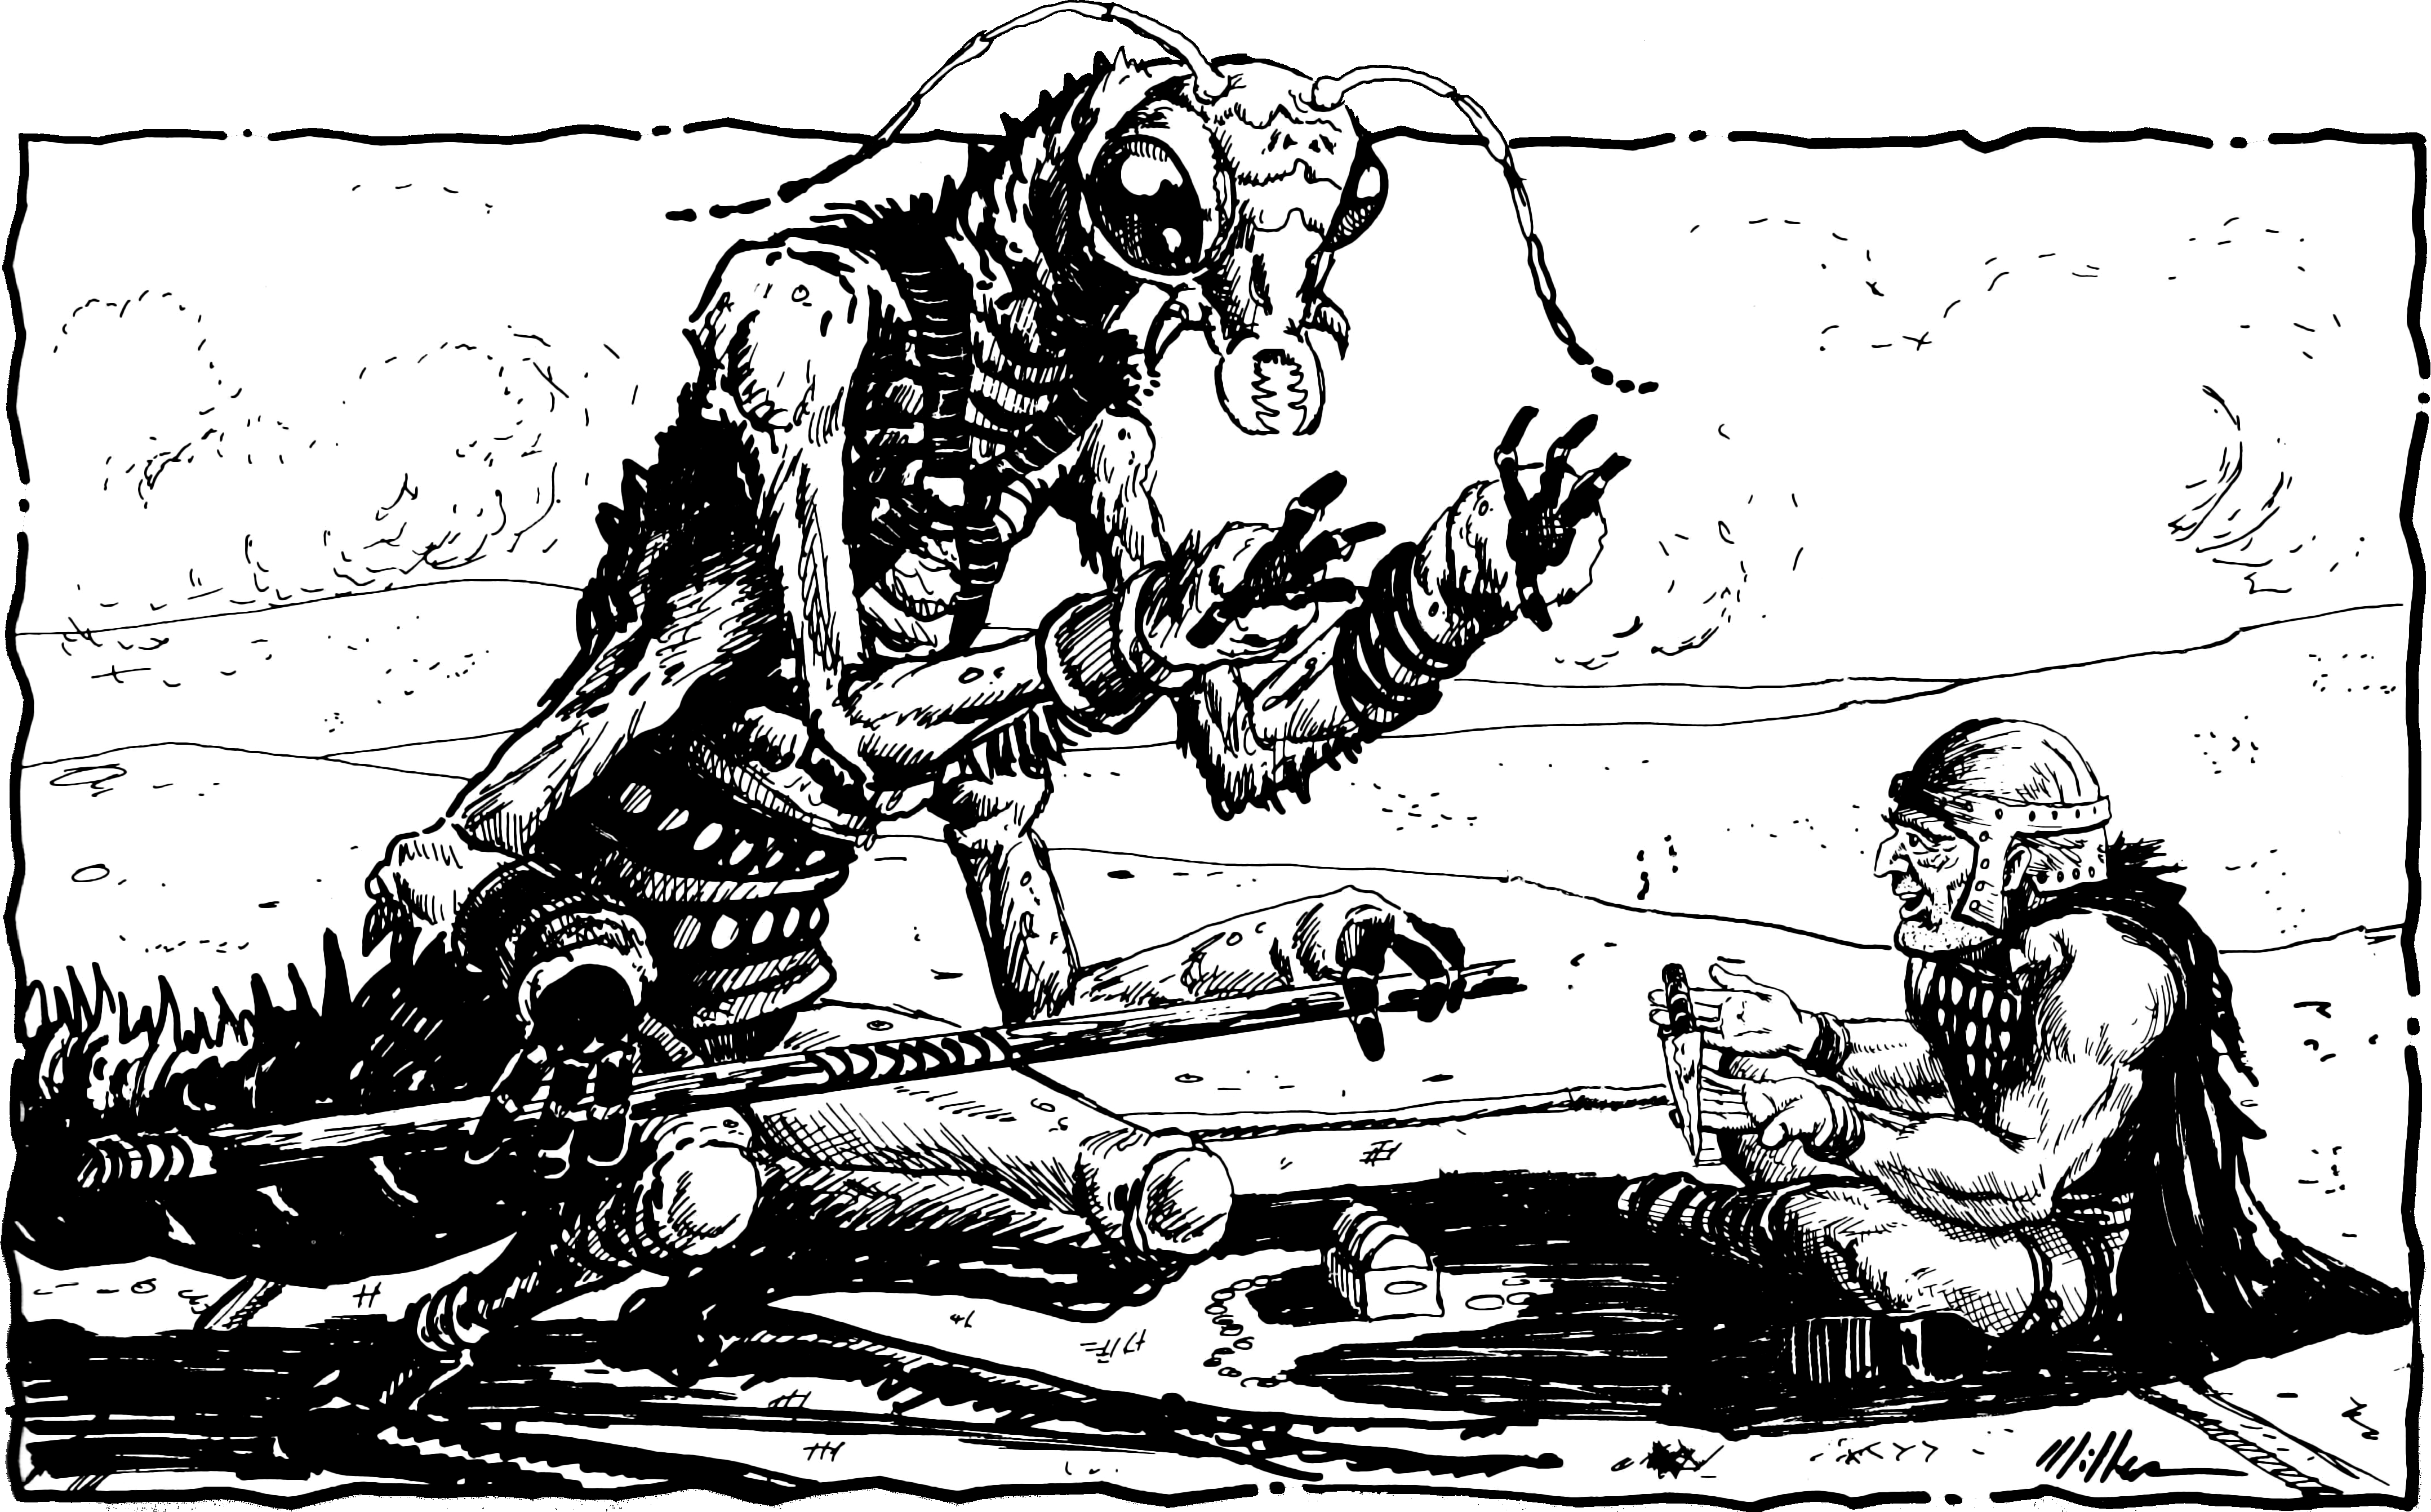
\includegraphics[width=\textwidth]{images/merchant-3.png}
\par\textit{\small\textcopyright Wizards of the Coast, 2020.}
\end{figure*}
\subsection{Documents}
This class of items has a symbolic function, conveying authority or permission. No price is listed for these items, because their value is not inherent.

\textbf{Letter of Marque}: This letter bears the personal mark of the sorcerer‐king, and bestows limited secular authority on the bearer, as if the bearer were a templar. The bearer of a letter of marque gains the authority to contest the actions of templars, using the bearer’s \skill{Diplomacy} check. If the bearer is already a templar, then having the letter as additional authority grants the templar a +4 circumstance check towards authority contest checks. The letter of marque does not grant the authority to Intrude, Requisition, Accuse or Judge, but does grant power to contest such actions by templars. A letter of marque is limited by time. After a specified period (usually one year, and never longer than seven years) the letter loses its effectiveness. A sorcerer‐king can also declare the letter invalid. Forging or fraudulently using a letter of marque is an unpardonable offense that brings a death sentence. Obviously, only the templars and other servants of the sorcerer‐king that issued the letter of marque will honor its terms. A person who is caught with a king’s letter of marque within another sorcerer‐king’s territory will have some explaining to do.

\textbf{Letter of Reprisal}: Like a letter of marque, this letter bears the personal mark of the sorcerer‐king, and bestows limited secular authority on the bearer, as if the bearer were a templar. Unlike a letter of marque, a letter of reprisal has a limited scope to carrying out a specific mission, usually a reprisal or retaliation against a specific group of the King’s enemies, for example, killing or capturing a specific enemy officer, capturing a particular enemy fortress or silt vessel, defiling a stretch of key farmland, or annihilating or enslaving a designated village. Depending on the bearer’s \skill{Diplomacy} ranks, she can Requisition, Intrude, Accuse, Judge, but only if she can show that her request relates to fulfilling her assigned mission. She can attempt to contest the actions of other templars, but takes a $-4$ circumstance penalty on such attempts, since the opposing templars can argue (even if it is not true) that she is acting outside of the scope of the assigned reprisal mission. The $-4$ penalty also applies if templars contest any of her Requisition, Intrude, Accuse, or Judge actions.
\subsectionA{Food, Drink, and Lodging}
Many Athasian travelers are lodged by merchant houses, elemental temples, psionic academies, or family. Adventurers, however, pay for hospitality.

\Table{Food, Drink, and Lodging}{XRR}{
\tableheader Item & \tableheader Cost & \tableheader Weight\\
\TableSubheader{Broy} &&\\
~ Keg (4 liters) & 2 cp & 5 kg\\
~ Mug & 4 bits & \onehalf kg\\
\TableSubheader{Inn stay (per day)} &&\\
~ Good & 2 sp & \\
~ Common & 5 cp & \\
~ Poor & 2 cp & \\
\TableSubheader{Meals (per day)} &&\\
~ Good & 5 bits & \\
~ Common & 3 bits & \\
~ Poor & 1 bit & \\
\TableSubheader{Water} &&\\
~ Keg (4 liters) & 2 bits & 5 kg\\
~ Mug & 1 bd & \onehalf kg\\
}

\textbf{Broy:} Broy is made from fermented kank nectar. Spiced broy and watered-down broy are also available. When served plain, it is potent and foul tasting. However, broy can be served warm and spiced with a pungent herb that disguises its sourness, as well as enhancing its enrapturing powers.

\textbf{Inn:} Poor accommodations at an inn amount to a place on the floor near the hearth. Common accommodations consist of a place on a raised, heated floor, the use of a blanket and a pillow. Good accommodations consist of a small, private room with one bed, some amenities, and a covered chamber pot in the corner.

\textbf{Meals:} Poor meals might be composed of bread, baked turnips, onions, and water. Common meals might consist of bread, chicken stew, carrots, and watered-down ale or wine. Good meals might be composed of bread and pastries, beef, peas, and ale or wine.
\subsectionA{Mounts and Related Gear}

\Table{Mounts and Related Gear}{XRR}{
\tableheader Goods or Services & \tableheader Cost & \tableheader Weight \\
\TableSubheader{Barding} &&\\
~ Medium creature & $\times$2 & $\times$1 \\
~ Large creature & $\times$4 & $\times$2 \\
Bit and bridle & 2 cp & \onehalf kg \\
Feed (per day) & 1 bit & 5 kg \\
\TableSubheader{Mounts} &&\\
~ \TableSubheader{Birds} &&\\
~ Erdland & 25 cp &\\
~ Erdlu & 10 cp &\\
~ \TableSubheader{Reptiles} &&\\
~ Crodlu, riding & 200 cp & \\
~ Crodlu, warmount & 400 cp & \\
~ Inix & 100 cp & \\
~ Mekillot & 200 cp & \\
~ \TableSubheader{Insects} &&\\
~ Kank, herding & 50 cp &\\
~ Kank, riding & 125 cp &\\
~ Kank, warmount & 250 cp &\\
\TableSubheader{Saddle} &&\\
~ Military & 20 cp & 15 kg \\
~ Pack & 5 cp & 7.5 kg \\
~ Riding & 10 cp & 12.5 kg \\
\TableSubheader{Saddle, Exotic} &&\\
~ Military & 60 cp & 20 kg \\
~ Pack & 15 cp & 10 kg \\
~ Riding & 30 cp & 15 kg \\
Saddlebags & 4 cp & 4 kg \\
Stabling (per day) & 5 bits &\\
}

\textbf{Barding, Medium Creature and Large Creature:} Barding is a type of armor that covers the head, neck, chest, body, and possibly legs of a horse or other mount. Barding made of medium or heavy armor provides better protection than light barding, but at the expense of speed. Barding can be made of any of the armor types found on \tabref{Armor and Shields}.

Armor for a horse (a Large nonhumanoid creature) costs four times as much as armor for a human (a Medium humanoid creature) and also weighs twice as much as the armor found on \tabref{Armor and Shields} (see Armor for Unusual Creatures). If the barding is for a pony or other Medium mount, the cost is only double, and the weight is the same as for Medium armor worn by a humanoid. Medium or heavy barding slows a mount that wears it, as shown on the table below.

Flying mounts can't fly in medium or heavy barding.

Removing and fitting barding takes five times as long as the figures given on \tabref{Donning Armor}. A barded animal cannot be used to carry any load other than the rider and normal saddlebags.

\Table{Barding}{XCCC}{
 & \multicolumn{3}{c}{\tableheader Base Speed}\\
\cmidrule[0.5pt]{2-4}
\tableheader Barding & \tableheader (12 m) & \tableheader (15 m) & \tableheader (18 m)\\
Medium & 9 m & 10.5 m & 12 m\\
Heavy & 9 m\footnotemark[1] & 10.5 m\footnotemark[1] & 12 m\footnotemark[1]\\

\TableNote{4}{1 A mount wearing heavy armor moves at only triple its normal speed when running instead of quadruple.}\\
}

\textbf{Crodlu:} A crodlu is a large bipedal lizard mount, resembling a scaled ostrich. A crodlu is appropriate as a mount for a Medium humanoid creature. Crodlu are hard to control in battle, while war crodlu can be ridden into battle easily. Crodlu benefit from stabling, can wear barding, and require feed like normal mounts.

\textbf{Erdland:} These creatures are large, flightless birds used as mounts or to pull caravans. They weigh around 2 tons and can stand up to 4.5 meters tall. An erdland is appropriate as a mount for a Medium humanoid creature. Erdlands can be ridden into battle easily. Erdlands benefit from stabling, can wear barding, and require feed like normal mounts.

\textbf{Erdlu:} Erdlus are a smaller variety of erdland, mostly used as herd beasts. They stand 2.1 meters tall and weigh around 100 kg. An erdlu is appropriate as a mount for a Medium humanoid creature. Erdlus are hard to control in battle. Erdlus benefit from stabling, can wear barding, and require feed like normal mounts.

\textbf{Feed:} Crodlus, erdlands, erdlus, inixes require feeding. Mekillots require eight times more than normal mounts.

\textbf{Inix:} The inix is a large, 5.5-meter long reptile commonly used for riding and as a beast of burden. An inix is appropriate as a mount for a Medium or Large humanoid creature. Inixes can be ridden into battle easily. Inixes benefit from stabling, can wear custom barding (specially constructed, adding an additional 50\% to the price), and require feed like normal mounts.

\textbf{Kank:} A kank is a large, 2.4-meter long insect, commonly used as a personal mount. These insects cannot be used as food, for their meat smells atrocious, but they produce highly nutritious globules of honey. A kank is appropriate as a mount for a Medium humanoid creature. Kanks are hard to control in battle. Kanks benefit from stabling, cannot wear barding, and do not require feeding.

\textbf{Mekillot:} A mekillot is a huge, 3,000-kg. lizard, used for hauling large cargo or serving as transportation for troops. These beasts are hard to control in combat and usually require a psionic handler. Mekillots benefit from stabling, can wear barding, and require feed eight times more than a normal mount.

\textbf{Saddle, Exotic:} An exotic saddle is like a normal saddle of the same sort except that it is designed for an unusual mount. Exotic saddles come in military, pack, and riding styles.

\textbf{Saddle, Military:} A military saddle braces the rider, providing advantage on \skill{Ride} checks related to staying in the saddle. If you're knocked unconscious while in a military saddle, you have a 75\% chance to stay in the saddle (compared to 50\% for a riding saddle).

\textbf{Saddle, Pack:} A pack saddle holds gear and supplies, but not a rider. It holds as much gear as the mount can carry.

\textbf{Saddle, Riding:} The standard riding saddle supports a rider.

\clearpage
\begin{figure}[t!]
\centering
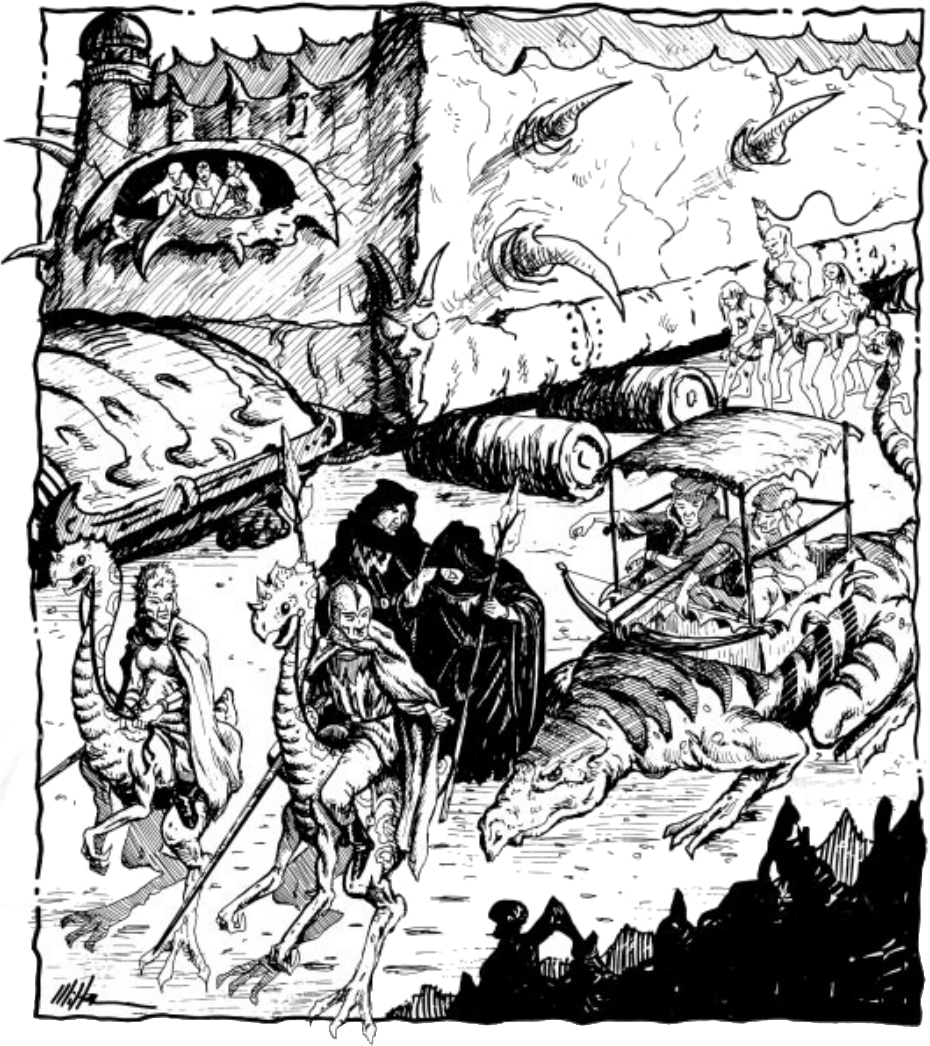
\includegraphics[width=\columnwidth]{images/caravan-3.png}
\par\textit{\small\textcopyright Wizards of the Coast, 2020.}
\end{figure}
\subsection{Transport}
Sometimes it is too hard or too dangerous to ride a kank---you'll need some other form of transportation. Some vehicles, such as the chariot and howdah, are moved by muscle power. The \skill{Handle Animal} skill is used only if that power comes from a team of draft animals. When the team consists of creatures with Intelligence scores of 3 or higher, the operative skill is \skill{Diplomacy}. When they are slaves or forced labor, the operative skill is \skill{Intimidate}.

\Table{Transport}{Xr{2cm}}{
\tableheader Transport & \tableheader Cost\\
Chariot, two-person, transport & 50 cp \\
Chariot, two-person, war & 125 cp \\
Chariot, four-person, war & 250 cp \\
Howdah, inix & 10 cp \\
Howdah, inix, war & 100 cp \\
Howdah, mekillot & 20 cp \\
Howdah, mekillot, war & 500 cp \\
Wagon, open, 500 kg capacity & 20 cp \\
Wagon, open, 1,250 kg capacity & 35 cp \\
Wagon, open, 2,500 kg capacity & 50 cp \\
Wagon, open, 5,000 kg capacity & 100 cp \\
Wagon, enclosed, 500 kg capacity & 40 cp \\
Wagon, enclosed, 1,250 kg capacity & 70 cp \\
Wagon, enclosed, 2,500 kg capacity & 100 cp \\
Wagon, enclosed, 5,000 kg capacity & 200 cp \\
Wagon, armored caravan & 1,000 cp \\
}

\textbf{Chariot}: A chariot is a two‐wheeled vehicle used for transportation, racing, war and processions. Transport chariots are very small and simple, requiring only a single animal to draw it. A war chariot built for two riders is slightly larger, but significantly better constructed. Generally one person will drive the chariot while the other uses a bow or other ranged weapon. A war chariot built for four is much larger than the other two kinds of chariots and requires at least two mounts to drive it. A war chariot offers cover to its occupants.

\textbf{Howdah}: A howdah is an enclosure mounted on a riding animal containing space for one or more persons. Howdahs can be fitted on inix or mekillots, and provide shade and cover from the elements. An inix howdah usually has room for only one person, though the war howdah, built much stronger, can hold four. A mekillot howdah can hold one or two persons, but a war howdah is much bigger, consisting of two levels and holding up to sixteen warriors.

\textbf{Wagon}: Wagons are an essential part of Athasian economy, as they facilitate the caravans that make life in the wastes possible. Open wagons are basic, open–topped wagons that can carry a certain amount of cargo. As Athasian wagons are built using little or no metal, there’s a limit to how much cargo they can carry. Open wagons generally require two beasts to draw them, but sometimes a single erdland will work.

\textit{Enclosed wagons}: They are more commonly used to transport people or fragile cargo that would otherwise be damaged by exposure to the elements.

\textit{Armored wagons}: They are primarily used by caravans traveling through areas plagued by dangerous monsters or raiders. It is an enclosed wagon with agafari wood used to strengthen the wagon throughout. There are also mount points for fixed crossbows on each side of that wagon that can swivel 180 degrees. Anyone using the crossbows or firing out of the rear of the wagon (when it is open) receives cover. Armored wagons require at least four smaller mounts to draw it, two inixes or one mekillot.

\subsectionA{Services}

\Table{Services}{lR}{
\tableheader Services & \tableheader Cost\\
Messenger         & 1 bit/km\\
Road or gate toll & 1 bit\\

\multicolumn{2}{l}{\TableSubheader{Hirelings, Military}}\\
Archer              & 1 bit/day  \\
Cavalry, heavy      & 3 bits/day \\
Cavalry, light      & 1 bit/day  \\
Crossbowman         & 5 bd/day   \\
Engineer            & 5 cp/day   \\
Infantry, heavy     & 5 bd/day   \\
Infantry, light     & 2 bd/day   \\
Infantry, irregular & 1 bd/day   \\

\multicolumn{2}{l}{\TableSubheader{Hirelings, Civilian}}\\
Draqoman                        & Level in cp/day \\
Craftsman\footnotemark[1]       & 1 bit/day      \\
Professional\footnotemark[2]    & 5 bd/day       \\
Specialist\footnotemark[3]      & 3 bits/day     \\
Spellcaster                     & 5 bits/day     \\
Unskilled labor\footnotemark[4] & 2 bd/day       \\


\multicolumn{2}{l}{\TableSubheader{Manifesting}}\\
Power, 1st--level & Manifester level $\times$ 10 cp\footnotemark[5]\\
Power, 2nd--level & Manifester level $\times$ 20 cp\footnotemark[5]\\
Power, 3rd--level & Manifester level $\times$ 30 cp\footnotemark[5]\\
Power, 4th--level & Manifester level $\times$ 40 cp\footnotemark[5]\\
Power, 5th--level & Manifester level $\times$ 50 cp\footnotemark[5]\\
Power, 6th--level & Manifester level $\times$ 60 cp\footnotemark[5]\\
Power, 7th--level & Manifester level $\times$ 70 cp\footnotemark[5]\\
Power, 8th--level & Manifester level $\times$ 80 cp\footnotemark[5]\\
Power, 9th--level & Manifester level $\times$ 90 cp\footnotemark[5]\\

\multicolumn{2}{l}{\TableSubheader{Spellcasting}}\\
Spell,   0--level & Caster level $\times$  5 sp\footnotemark[5]\footnotemark[6]\\
Spell, 1st--level & Caster level $\times$ 10 sp\footnotemark[5]\footnotemark[6]\\
Spell, 2nd--level & Caster level $\times$ 20 sp\footnotemark[5]\footnotemark[6]\\
Spell, 3rd--level & Caster level $\times$ 30 sp\footnotemark[5]\footnotemark[6]\\
Spell, 4th--level & Caster level $\times$ 40 sp\footnotemark[5]\footnotemark[6]\\
Spell, 5th--level & Caster level $\times$ 50 sp\footnotemark[5]\footnotemark[6]\\
Spell, 6th--level & Caster level $\times$ 60 sp\footnotemark[5]\footnotemark[6]\\
Spell, 7th--level & Caster level $\times$ 70 sp\footnotemark[5]\footnotemark[6]\\
Spell, 8th--level & Caster level $\times$ 80 sp\footnotemark[5]\footnotemark[6]\\
Spell, 9th--level & Caster level $\times$ 90 sp\footnotemark[5]\footnotemark[6]\\

\TableNote{2}{1 Any \skill{Craft} skill available.}\\
\TableNote{2}{2 Any \skill{Profession} skill available.}\\
\TableNote{2}{3 Any skill, other than Craft and Profession.}\\
\TableNote{2}{4 Jobs that do not require associated skills.}\\
\TableNote{2}{5 See its description for additional costs. If the additional costs put the total cost above 3,000 cp, that service is not generally available.}\\
\TableNote{2}{6 Spellcasting is considered high treason and spellcasters are not comfortable offering their services.}\\
}

Sometimes the best solution for a problem is to hire someone else to take care of it. Spellcasting, unless divine, is rarely, if ever, for sale on Athas. However, the manifesting of psionic powers for cash is much more common.

\textbf{Archer:} A 2nd-level fighter specialized in longbows, weilding a composite longbow (Str +2), and wearing studded leather and a buckler.

\textbf{Cavalry, Heavy:} A 2nd-level fighter wearing scale mail, and wielding a lance two-handed. They mount a heavy crodlu wearing a scale mail, as well.

\textbf{Cavalry, Light:} A 1st-level fighter wearing a studded leather and a wooden shield, and wielding a lance. They mount a light crodlu with no armor.

\textbf{Craftsman:} Usually a 2nd-level settler, but they can be of any class. This pays for any \skill{Craft} check of DC 20 or lower. Higher DC checks double the price for each 5 points of difference. 

\textbf{Crossbowman:} A 1st-level fighter specialized in crossbows, weilding a composite heavy crossbow (Str +4), and wearing studded scale mail and a tower shield.

\textbf{Draqoman:} A bard of 6th or higher level with at least one contact (see Alternative Class Features). Their wages depends on the bard's level and are the default price for skill contacts. If the draqoman has different types of contact, then they might double the price.

\textbf{Engineer:} A 5th-level fighter with 8 ranks of \skill{Knowledge} (warcraft) and a martial prowess that depend on this skill. They are equipped with \emph{breastplate +1} and a \emph{tower shield +1}. Although a military engineer has combat capabilities, their function is to oversee construction of siege engines and of static defenses.

\textbf{Infantry, Heavy:} A 2nd-level fighter, wearing a half-plate and tower shield, wielding a one-handed weapon. 

\textbf{Infantry, Light:} A 1st-level fighter, specialized either in spear and shields, or longswords. Light infantry usually wears studded leather, but caravan's infantry wear caravan armor.

\textbf{Infantry, Irregular:} A 2nd-level barbarian or gladiator. Their specialization is atypical, and they typically use gladiator armor or shell armor.

\textbf{Messenger:} This entry includes mounted messengers and runners. Those willing to carry a message to a place they were going anyway may ask for only half the indicated amount.

\textbf{Power:} The indicated amount is how much it costs to get a manifester to manifest a power for you. This cost assumes that you can go to the manifester and have the power manifested at his or her convenience. If you want to bring the manifester somewhere to manifest a power you need to negotiate with the manifester, otherwise the default answer is no.

The cost given is for a power with no XP cost. If the power has an XP cost, add 5 cp per XP lost.

Furthermore, if a power has dangerous consequences, the manifester will certainly require proof that you can and will pay for dealing with any such consequences (that is, assuming that the manifester even agrees to manifest such a power, which isn't certain). In the case of powers that transport the manifester and characters over a distance, you will likely have to pay for two manifestations of the power, even if you aren't returning with the manifester.

In addition, not every town or village has a manifester of sufficient level to manifest any power. In general, you must travel to a small town (or larger settlement) to be reasonably assured of finding a manifester capable of manifesting 1st--level powers, a large town for 2nd--level powers, a small city for 3rd-- or 4th--level powers, a large city for 5th-- or 6th--level powers, and a metropolis for 7th-- or 8th--level powers. Even a metropolis isn't guaranteed to have a local manifester able to cast 9th--level powers.

\textbf{Professional:} Usually a 2nd-level settler, but they can be of any class. This pays for any \skill{Profession} check of DC 20 or lower. Higher DC checks double the price for each 5 points of difference.

\textbf{Road or Gate Toll:} A toll is sometimes charged to cross a well-trodden, well-kept, and well-guarded road to pay for patrols on it and for its upkeep. Occasionally, a large walled city charges a toll to enter or exit (or sometimes just to enter).

\textbf{Specialist:} A 2nd-level NPC with \feat{Skill Focus} on the corresponding skill speciality, who can deliver a skill check of DC 20. Scouts are usually hired for \skill{Knowledge} (geography), \skill{Spot}, or \skill{Survival}. Thieves for \skill{Disable Device}, \skill{Forgery}, \skill{Open Lock}, \skill{Search}, or \skill{Sleight of Hand}. Bards for \skill{Appraise}, \skill{Diplomacy}, or \skill{Perform}. Wizards for \skill{Decipher Script}, any \skill{Knowledge}, or \skill{Spellcraft}. These are guidelines, but the wages are the same for any class.

\textbf{Spell:} The indicated amount is how much it costs to get a spellcaster to cast a spell for you. This cost assumes that you can go to the spellcaster and have the spell cast at his or her convenience (generally at least 24 hours later, so that the spellcaster has time to prepare the spell in question). If you want to bring the spellcaster somewhere to cast a spell you need to negotiate with him or her, and the default answer is no.

The cost given is for a spell with no cost for a material component or focus component and no XP cost. If the spell includes a material component, add the cost of that component to the cost of the spell.

If the spell has a focus component (other than a divine focus), add 1/10 the cost of that focus to the cost of the spell. If the spell has an XP cost, add 5 cp per XP lost.

Furthermore, if a spell has dangerous consequences, the spellcaster will certainly require proof that you can and will pay for dealing with any such consequences (that is, assuming that the spellcaster even agrees to cast such a spell, which isn't certain). In the case of spells that transport the caster and characters over a distance, you will likely have to pay for two castings of the spell, even if you aren't returning with the caster.

In addition, not every town or village has a spellcaster of sufficient level to cast any spell. In general, you must travel to a small town (or larger settlement) to be reasonably assured of finding a spellcaster capable of casting 1st--level spells, a large town for 2nd--level spells, a small city for 3rd-- or 4th--level spells, a large city for 5th-- or 6th--level spells, and a metropolis for 7th-- or 8th--level spells. Even a metropolis isn't guaranteed to have a local spellcaster able to cast 9th--level spells.

\textbf{Spellcaster:} A 3rd-level cleric or wizard. These wages do not pay for expensive material components, which must be given by the employer.

\textbf{Unskilled Labor:} Any job that a freeman might do that does not require a skill check.


\section{Special Materials}
A number of exotic materials can be found in the wilds and underground of the Tablelands and beyond, in addition to the more mundane ones. These substances have innate special properties. If you make a suit of armor or weapon out of more than one special material, you get the benefit of only the most prevalent material. However, you can build a double weapon with each head made of a different special material.

\subsection{Special Weapons Materials}
Each of the special materials described below has a definite game effect. Some creatures have damage reduction based on their creature type or core concept. Some are resistant to all but a special type of damage, such as that dealt by evil-aligned weapons or bludgeoning weapons. Others are vulnerable to weapons of a particular material. Characters may choose to carry several different types of weapons, depending upon the campaign and types of creatures they most commonly encounter.

\Table{Special Materials Cost Modifiers}{Xr{2.6cm}}{
\tableheader Type of Item & \tableheader Item Cost Modifier\\
\TableSubheader{Adamantine (dwarven steel)} &\\
Ammunition & +60 gp\\
Weapon & +3,000 gp\\
Shield & +2,000 gp\\
Light armor & +5,000 gp\\
Medium armor & +10,000 gp\\
Heavy armor & +15,000 gp\\

\TableSubheader{Agafari} &\\
Any wooden item & $\star$ + 20 cp per kg\\

\TableSubheader{Crystal, deep} &\\
Any weapon & +1,000 cp\\

\TableSubheader{Crystal, living} &\\
Ammunition & +250 cp\\
Light weapon & +750 gp\\
One-handed weapon, or one head of a double weapon & +1,000 gp\\
Two-handed weapon, or both heads of a double weapon & +1,500 gp\\
Light armor & +2,000 cp\\
Medium armor & +5,000 cp\\
Heavy armor & +9,000 cp\\

\TableSubheader{Crystal, mundane} &\\
Any armor, shield, or weapon & $\star$\\

\TableSubheader{Dasl} &\\
Any weapon & $\times$10\\

\TableSubheader{Drakehide} &\\
Any armor or shield & $\star$ $\times$ 2\\

\TableSubheader{Drake Ivory} &\\
Any weapon & $\times$2\\

\TableSubheader{Iron} &\\
Any armor, shield, or weapon & $\times$100\\

\TableSubheader{Silver, alchemical} &\\
Ammunition & +2 gp\\
Light weapon & +20 gp\\
One-handed weapon, or one head of a double weapon & +90 gp\\
Two-handed weapon, or both heads of a double weapon & +180 gp\\

\TableNote{2}{$\star$ Masterwork price}
}

\textbf{Adamantine}: While weapons and armor made from adamantine, also called ``dwarven steel'', can be found on Athas, they are quite rare. Nearly all items made from adamantine are relics from a long past age, scavenged from ruins by elves and treasure hunters. Raw adamantine cannot be bought on the market, and weapons and armor constructed from adamantine are considered priceless relics.

This ultrahard metal adds to the quality of a weapon or suit of armor. Weapons fashioned from adamantine have a natural ability to bypass hardness when sundering weapons or attacking objects, ignoring hardness less than 20. Armor made from adamantine grants its wearer damage reduction of 1/-- if it's light armor, 2/-- if it's medium armor, and 3/-- if it's heavy armor. Adamantine is so costly that weapons and armor made from it are always of masterwork quality; the masterwork cost is included in the prices. Thus, adamantine weapons and ammunition have a +1 enhancement bonus on attack rolls, and the armor check penalty of adamantine armor is lessened by 1 compared to ordinary armor of its type. Items without metal parts cannot be made from adamantine. An arrow could be made of adamantine, but a quarterstaff could not.

Only weapons, armor, and shields normally made of metal can be fashioned from adamantine. Weapons, armor and shields normally made of steel that are made of adamantine have one-third more hit points than normal. Adamantine has 40 hit points per inch of thickness and hardness 20.

\textbf{Agafari}: This rare magic wood is as hard as normal wood but very light. Any wooden or mostly wooden item (such as a bow, an arrow, or a spear) made from agadari is considered a masterwork item and weighs only half as much as a normal wooden item of that type. Items not normally made of wood or only partially of wood (such as a battleaxe or a mace) either cannot be made from agadari or do not gain any special benefit from being made of agadari. The armor check penalty of a agadari shield is lessened by 2 compared to an ordinary shield of its type. To determine the price of a agadari item, use the original weight but add 20 cp per kilogram to the price of a masterwork version of that item.

For weapons affected by the inferior material rule, agafari is considered an inferior material.

Agafari has 10 hit points per inch of thickness and hardness 5.

\textbf{Crystal, Deep}: Deep crystal is crystal of above-average quality found at the hearts of large veins or deposits of mundane crystal (see below). Deep crystal is renowned for its strength and its psionically resonant nature. Mundane crystal is used for many items of psionic manufacture, such as dorjes, power stones, and psicrystals. Deep crystal is a better grade.

While a weapon made of deep crystal is no different from a mundane crystal weapon for a nonpsionic character, a psionic wielder of a deep crystal weapon can focus psionic power through it, increasing the damage that weapon deals. As a free action that does not provoke attacks of opportunity, the wielder can channel psionic power into a melee weapon or ranged weapon made of deep crystal. For 2 power points, the deep crystal weapon deals an extra 2d6 points of damage. The weapon will stay charged for 1 minute or until it scores its next hit. Bows, crossbows, and slings bestow this power on their ammunition. All missile weapons lose this effect if they miss. However, they may be recovered and charged again.

Any weapon made of deep crystal costs 1,000 cp more than its noncrystal counterpart. Any item could potentially be made out of deep crystal. Because deep crystal armor is considered to be made out of metal, druids cannot wear it.

Deep crystal has 30 hit points per inch of thickness and hardness 10.

\textbf{Crystal, Living}: Living crystal is crystal of above-average quality renowned for its strength and its psionically-resonant nature. It is actually two different materials: the crystalline web material of a crystal spider used in making weapons, and the tissue of the crystal spider itself for making armor. The freshly-taken material must be treated within a day of its extraction by channeling psionic power into it, preserving its inherent psionic nature. One power point is required for every treated pound of material.

While a weapon made of living crystal is no different from a mundane crystal weapon (see below) for a nonpsionic character, a psionic wielder of a living crystal weapon can focus psionic power through it, increasing the damage that weapon deals. As a free action that does not provoke attacks of opportunity, and with the expediture of his psionic focus, the wielder can channel psionic power into a melee weapon or ranged weapon made of living crystal. For 2 power points, the living crystal weapon deals an extra 2d6 points of damage. The weapon will stay charged for 1 minute or until it scores its next hit. Bows, crossbows, and slings bestow this power on their ammunition. All missile weapons lose this effect if they miss. However, they may be recovered and charged again. For weapons affected by the inferior material rule, living crystal is considered inferior.

Armor made of living crystal is no different than metal armor for a nonpsionic character, but a psionic wearer of living crystal armor can focus psionic power through it, gaining an amount of damage reduction in the process. As a free action that does not provoke attacks of opportunity, and with the expediture of his psionic focus, the wearer can channel psionic power into armor made of living crystal. For 2 power points, the living crystal armor confers to the wearer damage reduction 5/metal. The armor will stay charged for 1 minute or until a hit is scored on it, whether or not the damage reduction applies to that particular hit. Unlike metal armor, living crystal armor isn't considered made of metal so druids can wear it without penalty.

Living crystal has 15 hit points per inch of thickness and hardness 8.

\textbf{Crystal, Mundane}: Mundane crystal can be used in place of metal in weapons or armor, using a special forging process. The fortified crystal possesses the properties of a similar masterwork steel weapon or armor, except for visual appearance.

Weapons and armor made of mundane crystal cost the same amount to make as their masterwork counterparts. Any item could potentially be made with mundane crystal. Because mundane crystal armor is considered to be made out of metal, druids cannot wear it.

Mundane crystal properly forged has 25 hit points per inch of thickness and a hardness of 8.

\textbf{Dasl}: Dasl is a special kind of crystalline material created by thri-kreen and often used to manufacture their weapons. An item made from dasl is treated as if it was made from iron and is not considered to be made from inferior materials. However, for purposes of harming creatures with damage reduction, a dasl weapon is not treated as being made from metal. An item made from dasl costs ten times what it normally would. Thus, a dasl chatkcha costs 200 cp instead of the 20 cp a stone or bone chatkcha would.

Dasl has a 15 hit points per inch of thickness and hardness 7.

\textbf{Drakehide}: The hide of a drake is of such value that most sorcerer-kings forbid their sale. They have instructed templars to confiscate any such items that appear in the market in the name of their sorcerer-king. Because drakes are so rare it is easy for templars to claim the item was stolen from the sorcerer-king and have the seller put to death. Elves, of course, defy these edicts at every turn, and make a fair profit selling drake materials while just one step ahead of their templar pursuers.

Armorsmiths can work with the hides of drakes to produce armor or shields of masterwork quality. One drake produces enough hide for four suits of hide armor, three suits of banded mail, two suits of half-plate, or one suit of full plate for a Medium creature. Enough hide is available to produce a small or large masterwork shield in addition to the armor.

Because dragonhide armor isn't made of metal, druids can wear it without penalty.

Drakehide armor costs double what masterwork armor of that type ordinarily costs, but it takes no longer to make than ordinary armor of that type.

Drakehide has 10 hit points per inch of thickness and hardness 10.

\textbf{Drake Ivory}: Drake ivory is extraordinarily strong and easy to work compared to the bone that most Athasian weaponsmiths use. Since it can only be obtained from the claws and teeth of deadly drakes, it is rare, expensive, and forbidden (see drakehide, above).

Weapons made from drake ivory cost an additional 2,000 cp to enchant. Weapons crafted from drake ivory cost twice what they normally would. A double weapon that is only half crafted using drake ivory increases its cost by 50\%.

Drake ivory has 30 hit points per inch of thickness and hardness 10.

% Giant Hair: Giant hair is very strong and frequently woven together to form a very strong cord. While sometimes used in armor, it is most frequently used to create rope. This rope costs 50 cp for 15 meters, has a hardness of 5 and 2 hp per inch of thickness

\textbf{Iron}: Iron (and most other metals) is rare on Athas, but weapons and armor made of iron can still be found. In all of the city-states, there are at least a few craftsmen that are able to work iron. The only fresh source of iron is the mines in the city-state of Tyr. Many of the iron weapons and armor available for sale have been scavenged from ruins. Weapons made of iron (including iron-based compounds like steel) can bypass the damage reduction possessed by some Athasian monsters. Iron-based items cost 100 times what they normally would.

Iron has 30 hit points per inch of thickness and hardness 10.

\textbf{Silver, Alchemical}: The process of binding silver to weapons has been greatly refined on Athas. Very little silver is actually needed in the process, and it can be bound to weapons crafted from dasl, obsidian and bone, as well as those made from iron.

A complex process involving metallurgy and alchemy can bond silver to a weapon made of steel so that it bypasses the damage reduction of creatures such as lycanthropes.

On a successful attack with a silvered weapon, the wielder takes a $-1$ penalty on the damage roll (with the usual minimum of 1 point of damage). The alchemical silvering process can't be applied to nonmetal items, and it doesn't work on rare metals such as adamantine, cold iron, and mithral.

Alchemical silver has 10 hit points per inch of thickness and hardness 8.
